%======================================================================
%  Rapport de Projet de Fin d'Etudes -- xQoS
%  Orchestration pilotee par l'intention dans un continuum
%  cloud-edge multi-fournisseurs
%
%  Compilation :  pdflatex main.tex && bibtex main && pdflatex main.tex x2
%  (ou : latexmk -pdf main.tex)
%
%  Fichiers utilises (voir rapport/README.md pour le detail du tri) :
%    main.tex          -- ce fichier, le document maitre
%    1_contexte.tex     -- Chapitre 1, contenu original : aaa.tex
%    2_architecture.tex -- Chapitre 2, contenu original : CHAPITRE2.tex
%    references.bib     -- bibliographie, sous-ensemble utilise de Bib.bib
%======================================================================
\documentclass[a4paper,12pt]{report}
\usepackage{amsmath}
\usepackage[T1]{fontenc}
%--- Encodage et langue ------------------------------------------------
\usepackage[utf8]{inputenc}
\DeclareUnicodeCharacter{202F}{\,}
\usepackage[french]{babel}
\usepackage{indentfirst}

%--- Mise en page --------------------------------------------------------
\usepackage[margin=2.5cm]{geometry}
\linespread{1.3}
\setcounter{tocdepth}{4}
\setcounter{secnumdepth}{4}

%--- Chapitres avec mini-sommaire (le bloc "Plan" en tete de chapitre) ---
\usepackage{minitoc}
\mtcsettitle{minitoc}{Plan}
\mtcsetrules{minitoc}{off}
\mtcsetfeature{minitoc}{before}{\vspace{-20pt}}
\dominitoc

%--- En-tetes de page (utilise par \lhead dans chaque chapitre) ---------
\usepackage{fancyhdr}

%--- Figures, tableaux, flottants ----------------------------------------
\usepackage{graphicx}
\graphicspath{{images/}}
\usepackage{booktabs}
\usepackage{float}
\usepackage[font={small,it}]{caption}

%--- Symboles de comparaison (tableau 1.1, comparatif de l'existant) ----
\usepackage{pifont}
\usepackage{xcolor}
\newcommand{\cmark}{\textcolor{green!60!black}{\ding{51}}}
\newcommand{\xmark}{\textcolor{red}{\ding{55}}}
\newcommand{\pmark}{\textcolor{orange}{$\sim$}}

%--- Liens et bibliographie ----------------------------------------------
\usepackage{url}
\usepackage[colorlinks=true]{hyperref}

\begin{document}

\rhead{\emph{}}

\tableofcontents
\listoffigures
\listoftables

\newpage
\pagestyle{fancy}

\lhead{\textsc{Chapitre 1. Contexte général}}
\renewcommand{\headrulewidth}{0.5pt}
\renewcommand{\footrulewidth}{0.5pt}
\chapter{Contexte général}\setlength{\headheight}{27.06pt}
\label{ch1}
\minitoc


\newpage
\section{Présentation de l'organisme d'accueil}
\label{sec:organisme}

Cette section est consacrée au LAAS-CNRS, laboratoire au sein duquel s'est déroulé notre projet de fin d'études pendant six mois.

\subsection{Présentation générale}

Le Laboratoire d'Analyse et d'Architecture des Systèmes (LAAS-CNRS)~\cite{laas_website}, comme illustré dans la figure~\ref{fig:logo-laas}, est un pôle d'excellence en automatique, informatique, robotique et micro/nanosciences.

\begin{figure}[H]
    \centering
    \includegraphics[width=0.35\textwidth]{images/LAAS.jpg}
    \caption{Logo du LAAS-CNRS}
    \label{fig:logo-laas}
\end{figure}

Sous la tutelle du Centre National de la Recherche Scientifique (CNRS), le LAAS-CNRS est associé à six membres fondateurs de l'Université de Toulouse (UT3 Paul Sabatier, INSA Toulouse, INP Toulouse, UT2J Jean Jaurès, UT1 Capitole) et opère sur un site unique, au 7 avenue du Colonel Roche à Toulouse. Comptant plusieurs centaines de chercheurs, enseignants-chercheurs, ingénieurs, techniciens et doctorants, dirigés par Mohamed Kaaniche, directeur de recherche CNRS, le LAAS-CNRS constitue l'un des plus importants laboratoires du CNRS en sciences de l'ingénieur.

Notre stage s'est déroulé au sein de l'équipe SARA (Services et Architectures pour Réseaux Avancés)~\cite{laas_sara}. Dirigée par Khalil Drira, cette équipe travaille sur les réseaux et systèmes de communication de nouvelle génération ; on y a travaillé sur leur plateforme, dotée du matériel nécessaire.



\subsection{Activités du LAAS-CNRS}

Structuré en six départements de recherche et vingt-quatre équipes, comme illustré à la figure~\ref{fig:departements-laas}, le LAAS-CNRS tire sa force de la diversité et de la complémentarité de ses expertises : Décision et Optimisation, Gestion de l'énergie, Systèmes hyperfréquences et photoniques, Micro Nano Bio Technologies, Réseaux/Informatique/Systèmes de confiance (dont dépend l'équipe SARA) et Robotique. Ses activités couvrent à la fois des recherches théoriques et des applications concrètes, trouvant des échos dans des domaines tels que l'aéronautique, l'espace, l'énergie, les transports, la santé et la défense, maintenant ainsi un lien étroit avec le tissu socio-économique.

\begin{figure}[H]
    \centering
    \includegraphics[width=0.85\textwidth]{images/Department.png}
    \caption{Départements de recherche au sein du LAAS-CNRS}
    \label{fig:departements-laas}
\end{figure}


L'encadrement de ce stage a été assuré par une équipe franco-tunisienne. Côté LAAS-CNRS, Christophe Chassot, Samir Medjiah et Sami Yangui ont suivi le projet ; M.Sami Yangui, maître de conférences à l'INSA Toulouse et membre du LAAS-CNRS, travaille sur les systèmes distribués, l'informatique orientée services et l'IoT, avec une spécialisation en cloud/edge computing et virtualisation des fonctions réseau. Côté ENIS Sfax, Mme Imene Lahyani, maîtresse de conférences et membre du laboratoire ReDCAD (Research laboratory on Development and Control of Distributed Applications), apporte son expertise en ingénierie logicielle des systèmes distribués et systèmes auto-adaptatifs ; les deux encadrantes ont d'ailleurs déjà co-publié sur le placement de services en edge computing, dans \emph{IEEE Transactions on Network and Service Management} (2024).

\section{Concepts de base}
Avant d'aborder la problématique spécifique de ce travail, il est nécessaire de poser précisément trois notions qui reviennent tout au long de ce rapport : le continuum cloud--edge--fog sur lequel repose l'architecture de notre projet, la qualité de service et les contrats qui la formalisent (QoS, SLO, SLA), et le paradigme d'orchestration piloté par l'intention qui guide la conception du système. Définir clairement ici ces notions évite toute confusion dans la suite du rapport.

\subsection{Le continuum cloud--edge--fog}
\label{sec:continuum}
L'architecture sur laquelle repose notre système s'appuie sur trois strates de calcul complémentaires : le cloud, le fog et l'edge, entre lesquelles une application peut aujourd'hui répartir ses traitements.

Le cloud computing centralise le calcul et le stockage dans de grands centres de données, accessibles à la demande selon un modèle de facturation à l'usage. Cette centralisation permet une mutualisation massive des ressources et une élasticité que peu d'infrastructures privées peuvent égaler, mais elle a un coût : les données doivent parcourir le réseau jusqu'au data center, souvent situé à des centaines de kilomètres, ce qui introduit une latence incompatible avec des applications comme la conduite autonome ou le contrôle industriel temps réel.

L'edge computing est né pour répondre à cette limite. Shi \emph{et al.}~\cite{shi2016edge} le définissent comme le fait d'exécuter les traitements à la périphérie du réseau, au plus près de la source des données, plutôt que de tout renvoyer vers un data center distant ; l'edge désigne alors toute ressource de calcul et de réseau située sur le chemin entre la source de données et le cloud, qu'il s'agisse d'un smartphone, d'une passerelle domestique ou d'un micro-data-center. Les objets connectés ne sont plus seulement consommateurs de contenu mais aussi producteurs de données, et l'edge doit traiter ces deux flux localement : l'enjeu est de réduire la latence, d'économiser la bande passante et de mieux protéger les données sensibles en évitant qu'elles ne transitent jusqu'au cloud.

Le fog computing poursuit la même logique, mais côté infrastructure plutôt que terminaux. Bonomi \emph{et al.}~\cite{bonomi2012fog}, qui ont introduit le terme, le définissent comme une plateforme virtualisée fournissant du calcul, du stockage et du réseau entre les terminaux et les data centers du cloud, typiquement en périphérie du réseau. Sa large répartition géographique, son grand nombre de nœuds hétérogènes, son support natif de la mobilité et son orientation temps réel le distinguent d'une simple extension du cloud. Le fog ne remplace donc pas ce dernier, il le prolonge vers la périphérie ; les deux paradigmes sont d'ailleurs souvent considérés comme interchangeables, l'edge étant davantage centré sur les objets et terminaux, le fog sur l'infrastructure intermédiaire qui les relie au cloud.

Ensemble, ces trois strates forment un continuum : un ensemble hiérarchisé et non figé de ressources allant des terminaux et nœuds edge jusqu'aux data centers cloud, en passant par des nœuds fog intermédiaires. Une application n'est plus assignée à un seul niveau ; elle peut répartir dynamiquement ses traitements selon ses contraintes de latence, de bande passante, de coût ou de disponibilité.

\subsection{QoS, SLO et SLA}
\label{sec:qos-slo-sla}
Les termes QoS, SLI, SLO et SLA reviennent constamment dans ce rapport, et sont souvent employés de façon interchangeable alors qu'ils recouvrent des réalités distinctes. Il convient donc de les définir précisément avant d'aller plus loin. On verra qu'ils forment une progression, de l'attente exprimée par l'utilisateur jusqu'à l'engagement contractuel du fournisseur.

\subsubsection{QoS (Quality of Service).} La qualité de service désigne l'ensemble des performances d'un service qui déterminent la satisfaction de son utilisateur. Dans le continuum, elle se traduit par ce qu'une application attend concrètement de son infrastructure : une latence faible, un débit suffisant, une disponibilité continue. C'est une notion large, qui exprime une attente plutôt qu'une valeur précise. Pour qu'un système puisse la garantir, il faut la rendre mesurable.

\subsubsection{SLI (Service Level Indicator).} Le SLI est la métrique que l'on mesure réellement sur le service. Il peut s'agir de la latence d'une requête, du taux d'erreur, du débit ou de la disponibilité. C'est lui qui rend la qualité observable, en la ramenant à des chiffres relevés en continu. Sans SLI, aucun objectif de qualité ne peut être vérifié.

\subsubsection{SLO (Service Level Objective).} Le SLO est la cible fixée sur un SLI. Il prend toujours la même forme : une métrique, un opérateur de comparaison et un seuil, comme \og~latence $\leq$ 100~ms~\fg{}. Cette structure simple suffit à transformer une attente qualitative en condition vérifiable automatiquement. À tout instant, le système peut donc dire si le SLO est respecté ou violé.

\subsubsection{SLA (Service Level Agreement).} La SLA est le contrat qui engage le fournisseur sur ses SLO. Ce qui la distingue d'un simple objectif interne, c'est la conséquence prévue en cas de non-respect : une pénalité financière, un remboursement, un dédommagement. Sans sanction, on parle de SLO ; avec sanction, de SLA. Cette distinction devient délicate lorsque plusieurs fournisseurs se partagent l'exécution d'une même application, car il devient difficile de désigner lequel est responsable d'une violation.

C'est cette chaîne -- la QoS comme attente, le SLI comme mesure, le SLO comme cible et la SLA comme garantie -- que xQoS doit reconstruire chez chaque fournisseur pour honorer l'intention exprimée par l'utilisateur.

\subsection{Orchestration pilotée par l'intention (intent-driven)}
\label{sec:intent-driven}

Une fois qu'on sait comment mesurer et garantir la qualité de service (QoS, SLO, SLA), il reste un problème : comment l'utilisateur communique-t-il ce qu'il veut au système ? C'est là qu'intervient la notion d'intention.

Une intention, c'est une expression de haut niveau du résultat voulu, sans dire comment l'atteindre. Plutôt que de préciser sur quel serveur déployer une application, avec combien de CPU, ou selon quelle règle migrer les traitements, l'utilisateur dit simplement ce qu'il attend : par exemple, \og~je veux un temps de réponse inférieur à 50~ms pour cette application~\fg{}. Toute la complexité technique -- le choix du nœud, du fournisseur, de la configuration -- reste cachée derrière cette phrase simple.

L'orchestration pilotée par l'intention, c'est le mécanisme qui prend cette intention et la transforme en actions concrètes. Ce mécanisme fait trois choses en continu : il traduit l'intention en objectifs mesurables (les SLO qu'on a définis avant), il choisit où et comment déployer pour satisfaire ces objectifs, et il surveille en permanence si l'intention reste respectée. Si ce n'est plus le cas -- un fournisseur devient trop lent, une ressource se sature -- il corrige automatiquement, en migrant ou en redéployant, sans que l'utilisateur ait à intervenir.



\section{Contexte et problématique}
\label{sec:problematique}

\subsection{Portée du projet}

Le travail présenté dans ce rapport s'inscrit dans la continuité des travaux de recherche menés par l'équipe SARA du LAAS-CNRS sur la gestion de la qualité de service dans le continuum cloud.

\subsection{Contexte}

L'Industrie 4.0 a transformé la production industrielle en s'appuyant sur les systèmes cyber-physiques, le cloud et l'intelligence artificielle pour créer des usines plus intelligentes, plus interconnectées et plus automatisées. L'Industrie 5.0 va plus loin en remettant l'humain au centre de cette boucle, avec une attention accrue portée à la collaboration homme-machine et à la résilience des systèmes de production. Ces évolutions, comme d'autres domaines critiques tels que les véhicules autonomes, la santé connectée ou la supervision industrielle en temps réel, reposent sur un même besoin : traiter les données au plus près de leur source. Le cloud seul, centralisé et souvent distant de plusieurs centaines de kilomètres, ne peut répondre à leurs exigences de latence, de bande passante ou de continuité de service~\cite{sfaxi2026policies}. Le continuum cloud-edge-fog répond à cette limite en répartissant les traitements sur plusieurs strates, chacune plus proche ou mieux adaptée à un besoin donné.

Cette répartition reste toutefois un potentiel, pas une garantie. Une application n'en tire réellement parti que si ses traitements sont placés au bon endroit, déplacés au bon moment et redimensionnés à mesure que les conditions évoluent. C'est le rôle de l'orchestration. Dans les systèmes actuels, elle repose sur des règles techniques fixées à l'avance -- un seuil d'utilisation CPU qui déclenche une réplication, un nombre de réplicas à maintenir, une contrainte de placement à respecter. Ces règles disent comment agir, jamais pourquoi : elles traduisent une décision prise en amont par un administrateur, et non le besoin réel de l'application. Dès que ce besoin change, il faut les redéfinir manuellement.

À cette difficulté s'ajoute une particularité du continuum, souvent passée sous silence : il n'appartient à aucun opérateur unique. Fournisseurs cloud, fournisseurs edge et fog, infrastructures industrielles privées y coexistent, chacun restant maître de ses propres ressources et de ses propres règles. Or la plupart des orchestrateurs actuels supposent l'inverse -- un domaine unique, dont ils contrôlent l'ensemble des ressources et connaissent l'état à tout instant. C'est de ce double constat que part notre projet : orchestrer les services à partir de l'intention exprimée par l'utilisateur plutôt que de règles figées, et le faire dans un environnement réparti entre plusieurs fournisseurs indépendants.

\subsection{Problématique}
\label{sec:problematique-sub}

Ces deux ambitions, prises ensemble, font apparaître une difficulté que ni l'une ni l'autre ne pose isolément. Une intention n'est pas une action ponctuelle à exécuter : c'est un objectif à tenir dans la durée. Or le fournisseur qui héberge une application aujourd'hui peut, demain, ne plus être en mesure de respecter cet objectif -- parce que ses ressources sont saturées, parce que sa charge a augmenté, ou parce que les conditions réseau se sont dégradées. L'intention doit alors être reprise ailleurs, chez un fournisseur capable de l'honorer, sans que l'utilisateur ait à la reformuler ni même à s'en apercevoir.

La difficulté tient à ce qu'aucun fournisseur ne commande aux autres. Chacun ne connaît que son propre domaine : il sait ce que ses machines peuvent offrir à un instant donné, mais ignore tout de l'état de ses pairs. Il n'existe donc ni vue d'ensemble sur laquelle s'appuyer pour choisir, ni autorité capable d'imposer un placement à l'ensemble des acteurs. La coordination ne peut pas être décidée d'en haut : elle doit émerger des fournisseurs eux-mêmes, à partir de ce que chacun accepte de déclarer sur ses propres capacités.

Deux risques apparaissent alors. D'abord, si chaque fournisseur reçoit l'intention sous une forme différente, ils s'engagent sans le savoir sur des objectifs qui ne sont pas les mêmes. Ensuite, si le passage d'un fournisseur à l'autre n'est pas encadré, une intention que personne ne peut satisfaire risque de circuler sans fin entre eux, sans jamais aboutir ni être déclarée impossible.

La question qui structure ce travail est donc la suivante : comment faire coopérer des fournisseurs indépendants autour d'une même intention -- la leur transmettre sans ambiguïté, comparer ce que chacun peut offrir, désigner le mieux placé, puis passer le relais quand les conditions changent -- alors qu'aucun d'eux ne commande aux autres ?

%% ===================================================================
%% 1.4 Étude des solutions existantes
%% ===================================================================
\section{Étude de l'existant}
\label{sec:etat-art}

De nombreuses plateformes traitent déjà l'orchestration de services dans le continuum cloud-edge. Elles automatisent le déploiement, le placement et la supervision des applications distribuées, et adaptent dynamiquement les ressources allouées à l'évolution des conditions d'exécution. Nous en présentons ci-dessous trois, retenues parce qu'elles représentent chacune une réponse différente au problème d'orchestration, et parce qu'elles permettent de situer précisément la limite identifiée dans notre problématique (sous-section~\ref{sec:problematique-sub}).

\subsection{Kubernetes et KubeEdge}
\label{sec:etat-art-k8s}

Kubernetes~\cite{website:kubernetes} est aujourd'hui l'orchestrateur de conteneurs de référence dans l'industrie. Il repose sur un modèle déclaratif : l'utilisateur décrit l'état souhaité de son application, et le système converge automatiquement vers cet état en déployant, redémarrant ou répliquant les conteneurs. Son extension KubeEdge~\cite{website:kubeedge} prolonge ce fonctionnement jusqu'aux nœuds edge, permettant de gérer depuis un plan de contrôle central des ressources situées en périphérie du réseau, comme l'illustre la figure~\ref{fig:kubernetes}.

\begin{figure}[H]
    \centering
    % \includegraphics[width=0.75\textwidth]{images/kubernetes.png}
    \caption{Architecture de Kubernetes étendue à l'edge par KubeEdge}
    \label{fig:kubernetes}
\end{figure}

Ce modèle apporte une réponse robuste à l'hétérogénéité technique du continuum : Kubernetes sait placer une charge sur des nœuds aux capacités variables et réagir à leur défaillance. En revanche, ce que l'utilisateur déclare demeure de nature technique -- un nombre de réplicas, une quantité de CPU, une contrainte de placement -- et non une intention exprimée en termes de qualité de service. Surtout, Kubernetes repose sur un plan de contrôle central qui possède la vue complète des ressources et décide seul de leur affectation. C'est précisément l'hypothèse que notre contexte invalide : dans un continuum réparti entre plusieurs fournisseurs indépendants, aucun acteur ne dispose de cette vue globale ni du pouvoir d'imposer un placement aux autres.

\subsection{ONAP (Open Network Automation Platform)}
\label{sec:etat-art-onap}

ONAP~\cite{website:onap} est une plateforme industrielle d'orchestration de services réseau, portée par la Linux Foundation et adoptée par plusieurs grands opérateurs télécoms. Elle couvre l'ensemble du cycle de vie des services, intègre une gestion des politiques et des SLA, et propose une approche \emph{intent-based} à travers un module dédié à la gestion des intentions, comme le montre la figure~\ref{fig:onap}.

\begin{figure}[H]
    \centering
    % \includegraphics[width=0.75\textwidth]{images/onap.png}
    \caption{Architecture fonctionnelle de la plateforme ONAP}
    \label{fig:onap}
\end{figure}

ONAP se rapproche donc de notre problématique sur un point : elle reconnaît explicitement la notion d'intention et traite les engagements de qualité de service comme des objets de premier plan. Deux limites subsistent néanmoins. L'intention y est traduite vers un ensemble de politiques prédéfinies, selon des règles de correspondance configurées à l'avance, plutôt qu'évaluée au regard des capacités réellement disponibles au moment de la décision. Par ailleurs, la plateforme est conçue pour l'environnement d'un opérateur unique, qui orchestre ses propres ressources : la coopération entre fournisseurs autonomes, chacun décidant seul de ce qu'il accepte de prendre en charge, n'entre pas dans son périmètre.

\subsection{IntentContinuum}
\label{sec:etat-art-intentcontinuum}

IntentContinuum~\cite{akbari2025intentcontinuum} est un prototype de recherche récent, qui propose d'utiliser un grand modèle de langage pour interpréter les intentions exprimées par l'utilisateur et adapter en conséquence le placement des services dans le continuum. Le système surveille en continu le respect de l'intention et, en cas de violation, sollicite le modèle de langage pour analyser la cause du problème et sélectionner une action corrective.

C'est la solution la plus proche conceptuellement de notre approche, puisqu'elle place l'intention au cœur de l'orchestration et met en œuvre une boucle de rétroaction continue. Elle reste toutefois construite autour d'un décideur unique, qui connaît l'ensemble des ressources et choisit à lui seul où placer les services : la question du passage de relais entre fournisseurs indépendants, lorsque celui qui héberge l'application ne peut plus tenir ses engagements, ne s'y pose jamais. Le modèle de langage y assure en outre à la fois l'interprétation et la décision de placement, ce qui rend le raisonnement difficile à auditer et l'explicabilité limitée à des justifications textuelles non structurées.

\subsection{Synthèse comparative}
\label{sec:etat-art-synthese}

Le tableau~\ref{tab:comparatif-existant} compare ces trois solutions selon les critères qui structurent notre travail.

\begin{table}[H]
    \centering
    \caption{Comparatif synthétique des solutions d'orchestration étudiées}
    \label{tab:comparatif-existant}
    \begin{tabular}{p{5.5cm}ccc}
        \toprule
        \textbf{Critère} & \textbf{Kubernetes} & \textbf{ONAP} & \textbf{IntentContinuum} \\
        \midrule
        Orchestration du continuum edge-cloud & \cmark & \cmark & \cmark \\
        Pilotage par l'intention utilisateur & \xmark & \pmark & \cmark \\
        Coordination entre fournisseurs autonomes & \xmark & \pmark & \xmark \\
        Décision sans autorité centrale & \xmark & \xmark & \xmark \\
        Passage de relais entre fournisseurs & \xmark & \xmark & \xmark \\
        Décision proactive fondée sur la prédiction & \xmark & \xmark & \pmark \\
        Explicabilité des décisions & \xmark & \xmark & \pmark \\
        \bottomrule
    \end{tabular}
    \\[0.3cm]
    {\footnotesize \cmark~: pris en charge \quad \pmark~: partiellement pris en charge \quad \xmark~: non pris en charge}
\end{table}

Cette comparaison confirme le constat posé en problématique : aucune des solutions étudiées ne traite la coordination entre fournisseurs autonomes. Toutes reposent, sous des formes différentes, sur un décideur unique disposant d'une vue complète des ressources et du pouvoir de les affecter -- un plan de contrôle central chez Kubernetes, l'orchestrateur d'un opérateur chez ONAP, le système lui-même chez IntentContinuum. Aucune ne prévoit qu'un fournisseur puisse refuser une intention, proposer sa propre offre, ou transmettre à un pair une charge qu'il n'est plus en mesure d'honorer. C'est au regard de cette limite commune que nous avons conçu la solution présentée dans la section~\ref{sec:solution}
\section{Solution proposée}
\label{sec:solution}
Pour répondre à cette problématique, nous avons développé xQoS, un prototype d'orchestrateur réparti entre plusieurs fournisseurs, où chacun conserve la maîtrise de ses propres ressources.

Le point de départ est l'intention de l'utilisateur, exprimée en langage naturel — par exemple une contrainte de latence pour une application donnée. Le fournisseur qui la reçoit la traduit en objectifs chiffrés et vérifiables, puis diffuse ces objectifs à l'ensemble des autres fournisseurs. La traduction n'est donc faite qu'une seule fois : tous travaillent ensuite sur le même contrat, ce qui écarte le risque que chacun s'engage sur une interprétation différente de la même demande.

Vient ensuite le choix du fournisseur. Plutôt qu'une autorité centrale qui imposerait un placement, xQoS interroge tous les fournisseurs en parallèle et laisse chacun répondre par une offre, établie à partir des seules ressources qu'il connaît : les siennes. Ces offres sont comparées selon plusieurs critères simultanément, et le fournisseur le mieux placé se voit confier l'application. La décision émerge ainsi des propositions des fournisseurs eux-mêmes, sans qu'aucun ne décide pour les autres.

Une fois l'application déployée, xQoS ne se contente pas d'attendre qu'un problème survienne. Il surveille en continu les indicateurs pertinents et anticipe les dégradations, de manière à réagir avant que l'objectif ne soit violé. Si le fournisseur en place n'est plus en mesure de tenir ses engagements, l'intention est transmise à un autre, qui reprend la main. Ce passage de relais est encadré : un fournisseur déjà sollicité pour une intention donnée ne peut être resollicité, ce qui évite qu'une intention impossible à satisfaire ne circule indéfiniment entre les fournisseurs.

Enfin, chaque étape reste consultable : la façon dont l'intention a été comprise, les offres reçues, la raison pour laquelle tel fournisseur a été retenu, et ce qui a motivé chaque passage de relais. L'utilisateur, comme l'opérateur, dispose ainsi des éléments nécessaires pour vérifier que la demande initiale a bien été honorée.

Les exigences que ces choix imposent au système sont précisées dans la section suivante, avant la présentation de l'architecture en section~\ref{sec:architecture}.
\section{Méthodologie de travail}
\label{sec:methodologie}

Le choix d'une méthodologie de développement adaptée conditionne la qualité du travail réalisé et le respect des délais. Pour ce projet, nous avons retenu la méthodologie agile Scrum~\cite{schwaber2020scrumguide}, qui privilégie des livraisons fréquentes et incrémentales plutôt qu'une spécification figée en amont -- un choix particulièrement adapté à un projet de recherche, où les besoins se précisent à mesure que le prototype se construit.

\subsection{Principes de Scrum}

Scrum organise le développement en itérations courtes appelées \emph{sprints}, chacune aboutissant à un incrément fonctionnel du produit. Le travail à réaliser est consigné dans un \emph{product backlog}, dont une partie est sélectionnée à chaque début de sprint pour constituer le \emph{sprint backlog}. Le déroulement du sprint est ponctué de réunions courtes et régulières : une réunion de planification à l'ouverture, des points quotidiens de synchronisation, puis une revue et une rétrospective à la clôture~\cite{schwaber2001agile}, comme l'illustre la figure~\ref{fig:scrum}.

\begin{figure}[H]
    \centering
    % \includegraphics[width=0.75\textwidth]{images/methode-scrum.jpg}
    \caption{Processus de la méthodologie Scrum}
    \label{fig:scrum}
\end{figure}

\subsection{Rôles et responsabilités}

La répartition des rôles au sein du projet est présentée dans le tableau~\ref{tab:roles}.

\begin{table}[H]
    \centering
    \caption{Rôles et responsabilités dans la mise en œuvre du projet}
    \label{tab:roles}
    \begin{tabular}{p{6cm}p{7cm}}
        \toprule
        \textbf{Rôle / Responsabilité} & \textbf{Personne responsable} \\
        \midrule
        Orientation scientifique et validation & M. Sami YANGUI \\
        Encadrement technique & M. Samir MEDJIAH \\
        Encadrement académique & Mme Imene LAHYANI \\
        Conception et développement & Mustapha Amine KECHAOU \\
        Conception et développement & Ahmed KAMMOUN \\
        \bottomrule
    \end{tabular}
\end{table}

\subsection{Suivi et réunions}

Le projet a été suivi par des réunions régulières associant les encadrants et les deux développeurs. Le tableau~\ref{tab:reunions} récapitule la nature de ces réunions et leurs participants.

\begin{table}[H]
    \centering
    \caption{Réunions de suivi et participants}
    \label{tab:reunions}
    \begin{tabular}{p{4cm}p{3cm}p{6.5cm}}
        \toprule
        \textbf{Type de réunion} & \textbf{Fréquence} & \textbf{Participants} \\
        \midrule
        Point de synchronisation & Quotidienne & Mustapha Amine KECHAOU, Ahmed KAMMOUN \\
        Revue technique & Hebdomadaire & Binôme, M. Samir MEDJIAH \\
        Revue de sprint & Fin de sprint & Binôme, M. Sami YANGUI, M. Samir MEDJIAH,Mme.Imene LAHYANI \\
        \bottomrule
    \end{tabular}
\end{table}

\subsection{Planification des sprints}

Le développement a été organisé en sprints successifs, chacun ciblant un ensemble cohérent de fonctionnalités. Le tableau~\ref{tab:sprints} récapitule ce découpage.

\begin{table}[H]
    \centering
    \caption{Planification des sprints}
    \label{tab:sprints}
    \begin{tabular}{p{2cm}p{8.5cm}p{3.5cm}}
        \toprule
        \textbf{Sprint} & \textbf{Activités réalisées} & \textbf{Durée} \\
        \midrule
        Sprint 0 &
        - Étude de l'état de l'art sur l'orchestration du continuum \newline
        - Analyse du cahier des charges \newline
        - Préparation de l'environnement de développement &
        16 février -- 1\textsuperscript{er} mars 2026 \\
        \midrule
        Sprint 1 &
        - Mise en place du hub central et des microservices \newline
        - Collecte des métriques système et réseau \newline
        - Persistance des données &
        2 mars -- 22 mars 2026 \\
        \midrule
        Sprint 2 &
        - Traduction des intentions en langage naturel vers des SLO \newline
        - Intégration d'un modèle de langage local \newline
        - Fusion des intentions successives &
        23 mars -- 12 avril 2026 \\
        \midrule
        Sprint 3 &
        - Détection des violations de SLO \newline
        - Prédiction des dégradations à venir \newline
        - Déclenchement proactif des migrations &
        13 avril -- 3 mai 2026 \\
        \midrule
        Sprint 4 &
        - Évaluation multicritère des cibles candidates \newline
        - Sélection de la cible de migration \newline
        - Prévention des migrations en cascade &
        4 mai -- 24 mai 2026 \\
        \midrule
        Sprint 5 &
        - Diffusion des intentions entre fournisseurs \newline
        - Collecte et comparaison des offres \newline
        - Attribution au fournisseur retenu &
        25 mai -- 14 juin 2026 \\
        \midrule
        Sprint 6 &
        - Passage de relais entre fournisseurs \newline
        - Protection contre les boucles de transmission \newline
        - Validation des scénarios multi-provider &
        15 juin -- 5 juillet 2026 \\
        \midrule
        Sprint 7 &
        - Tableau de bord d'observabilité \newline
        - Traçabilité des décisions prises \newline
        - Tests d'intégration &
        6 juillet -- 26 juillet 2026 \\
        \midrule
        Sprint 8 &
        - Rédaction du rapport \newline
        - Préparation de la soutenance &
        27 juillet -- 16 août 2026 \\
        \bottomrule
    \end{tabular}
\end{table}
\section{Conclusion}
Ce premier chapitre a posé le cadre du travail présenté dans ce rapport. Après avoir présenté le LAAS-CNRS et l'équipe SARA au sein de laquelle s'est déroulé ce stage, nous avons défini les notions qui reviennent tout au long du document : le continuum cloud-edge-fog, la chaîne QoS-SLI-SLO-SLA, et le principe de l'orchestration pilotée par l'intention.

Ces notions nous ont permis de formuler la problématique : dans un continuum réparti entre plusieurs fournisseurs indépendants, où aucun ne commande aux autres, comment faire coopérer ces acteurs autour d'une même intention — la leur transmettre, comparer ce que chacun peut offrir, désigner le mieux placé, puis passer le relais lorsque les conditions changent ?

L'étude des solutions existantes a confirmé que cette question reste ouverte : Kubernetes, ONAP et IntentContinuum reposent toutes, sous des formes différentes, sur un décideur unique disposant d'une vue complète des ressources. Nous avons alors présenté xQoS, le prototype développé durant ce stage, ainsi que la méthodologie de travail suivie.

\newpage
\pagestyle{fancy}

\lhead{\textsc{Chapitre 2. Architecture générale de la plateforme}}
\renewcommand{\headrulewidth}{0.5pt}
\renewcommand{\footrulewidth}{0.5pt}
\chapter{Architecture générale de la plateforme}\setlength{\headheight}{27.06pt}
\label{ch2}
\minitoc


\newpage
\section{Inroduction}
\label{sec:architecture}

La plateforme développée durant ce stage maintient un service applicatif de streaming au service d'un véhicule autonome en mouvement, en le déplaçant au fil du temps vers la machine la mieux adaptée parmi celles qu'offrent deux fournisseurs distincts. Cette section décrit comment la plateforme est structurée pour y parvenir : d'abord l'environnement sur lequel elle agit, puis le style architectural retenu, le rôle du composant central et celui des services qui l'entourent, les composants qui la relient à l'infrastructure réelle, et enfin la façon dont l'ensemble est dupliqué pour couvrir les deux fournisseurs. Les mécanismes internes de chaque composant seront détaillés dans les chapitres suivants.

\section{L'environnement d'exécution}
\label{sec:environnement}

La plateforme n'a de sens que rapportée à l'environnement dans lequel elle s'exécute. Cet environnement se compose d'un véhicule autonome qui circule sur une carte, d'un service applicatif qui le pilote, et d'un ensemble de machines virtuelles réparties sur cette même carte -- certaines en périphérie, au plus près du terrain, d'autres plus éloignées mais mieux dotées en ressources. Le service est hébergé sur l'une de ces machines à la fois, et rien n'impose qu'il y reste : à mesure que le véhicule se déplace et s'éloigne de son hôte actuel, une autre machine peut devenir un meilleur choix. Toute la question est de savoir quand basculer, et vers laquelle.

\subsection{Le terminal mobile}
\label{sec:picarx}

Le client du service est un véhicule autonome PiCar-X, une plateforme robotique fondée sur un Raspberry Pi, équipée d'une caméra sur deux axes, d'un module à ultrasons et de capteurs de suivi de ligne~\cite{sunfounder_picarx}. Ce choix n'est pas anecdotique : il fournit un cas d'usage où la contrainte de latence est réelle et non posée par convention, puisqu'un véhicule qui décide de sa trajectoire ne peut pas attendre indéfiniment la réponse du service qui le pilote.

Le véhicule circule en continu le long d'une trajectoire fermée tracée sur la carte, passant successivement à proximité de chacune des machines qui y sont positionnées. C'est ce déplacement qui rend le problème intéressant : la machine idéale à un instant donné cesse de l'être quelques secondes plus tard, sans qu'aucune ressource n'ait changé d'état -- seule la position du client a changé. Le placement du service doit donc être réévalué en permanence, et non fixé une fois pour toutes au déploiement.

\paragraph{Du ping réseau à la carte simulée.} Dans une première version, la latence était mesurée par de simples pings ICMP vers chaque machine. Deux difficultés sont rapidement apparues : rien ne permettait de vérifier si les valeurs obtenues étaient cohérentes, et surtout il devenait impossible de les maîtriser lors d'une démonstration, le système subissant les aléas du réseau réel. Nous avons donc opté pour une carte simulée, sur laquelle chaque machine se voit attribuer une position fixe et le véhicule une position courante : la distance qui les sépare devient ainsi calculable à tout instant.

\paragraph{Le mécanisme de mesure.} Le calcul du RTT (round-trip time) suit un échange simple entre le véhicule et la machine visée, illustré par le diagramme de séquence de la figure~\ref{fig:calcul-rtt}. À l'instant $t_0$, le véhicule envoie sa position $(x,y)$ à la machine par une requête POST. Celle-ci reçoit la position, calcule la distance qui l'en sépare, puis attend -- \texttt{sleep(f(distance))} -- une durée fonction de cette distance, avant de répondre. Le véhicule reçoit la réponse à l'instant $t_1$. Le RTT mesuré est alors $t_1 - t_0$ : un délai réellement subi par l'attente introduite côté serveur, et non une valeur affichée après coup. C'est cette attente contrôlée qui permet de simuler une latence réseau réaliste sans dépendre des aléas d'un réseau physique.

\begin{figure}[H]
    \centering
    % \includegraphics[width=0.85\textwidth]{images/calcul_rtt.png}
    \caption{Diagramme de séquence du calcul du RTT entre le véhicule et une machine}
    \label{fig:calcul-rtt}
\end{figure}

\paragraph{Le modèle de latence.} Au début du projet, la fonction régissant ce délai était calculée par une simple règle de trois -- par exemple, 10 m correspondant à 200 ms. Le problème est apparu rapidement : lorsque la distance devient nulle, c'est-à-dire lorsque le véhicule atteint physiquement la machine, le sleep calculé devient nul lui aussi, produisant un RTT quasiment nul. Cette valeur est absurde : aucune latence réseau, même locale, n'est jamais réellement nulle.

Le modèle retenu résout ce problème en imposant deux bornes non nulles à chaque extrémité, comme le montre la figure~\ref{fig:calcul-sleep-formule} : une distance minimale $D_{min}$ associée à un délai minimal $T_{min}$, tous deux différents de zéro, et une distance maximale $D_{max}$ associée à un délai maximal $T_{max}$. Entre ces deux bornes, le délai est obtenu par interpolation linéaire :

\begin{equation}
t = \frac{x - D_{min}}{D_{max} - D_{min}} \times (T_{max} - T_{min}) + T_{min}
\label{eq:sleep-formule}
\end{equation}

où $x$ est la distance mesurée. En dehors de l'intervalle $[D_{min}, D_{max}]$, la distance est d'abord ramenée à sa borne la plus proche, de sorte que le délai reste toujours compris entre $T_{min}$ et $T_{max}$, jamais nul et jamais illimité.

\begin{figure}[H]
    \centering
    % \includegraphics[width=0.75\textwidth]{images/calcul_sleep_formule.png}
    \caption{Interpolation entre bornes non nulles pour le calcul du délai simulé}
    \label{fig:calcul-sleep-formule}
\end{figure}

\begin{figure}[H]
    \centering
    %\includegraphics[width=0.85\textwidth]{images/latence_regle_de_trois.png}
    \caption{Modèle de latence retenu (edge et cloud) comparé à la règle de trois naïve}
    \label{fig:latence-regle-trois}
\end{figure}

Les paramètres retenus figurent dans le tableau~\ref{tab:params-latence}.

\begin{table}[H]
    \centering
    \caption{Paramètres du modèle de latence}
    \label{tab:params-latence}
    \begin{tabular}{llcc}
        \toprule
        \textbf{Paramètre} & \textbf{Symbole} & \textbf{Edge} & \textbf{Cloud} \\
        \midrule
        Distance minimale & $D_{min}$ & 3 cm & 3 cm \\
        Distance maximale & $D_{max}$ & 80 cm & 80 cm \\
        Latence minimale & $B$ & 5 ms & 50 ms \\
        Latence maximale & $A$ & 150 ms & 230 ms \\
        \bottomrule
    \end{tabular}
\end{table}

Ce modèle est appliqué de façon identique aux huit machines, mais avec des bornes différentes selon leur niveau : une machine edge répond entre 5 et 150 ms, une machine cloud entre 50 et 230 ms, ce qui traduit une réalité physique -- une ressource cloud demeure structurellement plus éloignée, quelle que soit la position du véhicule. La conséquence est visible sur la figure~\ref{fig:latence-regle-trois} : les deux courbes ne se croisent jamais, et à distance égale, le cloud reste toujours plus latent que l'edge. Mais cela ne signifie pas que la machine la plus proche est toujours la meilleure candidate : un nœud edge proche peut malgré tout être surchargé, ce qui justifie l'évaluation multicritère présentée plus loin, où la latence n'est qu'un critère parmi d'autres.
\subsection{L'infrastructure d'accueil}
\label{sec:infra-accueil}

Les machines virtuelles décrites plus haut ne tournent pas sur une infrastructure fictive : elles sont hébergées sur CROcc (Cloud Recherche Occitanie), la plateforme cloud du datacenter régional occitan (DROcc), opérée en partenariat entre Toulouse et Montpellier et rattachée à la fédération de clouds académiques France Grilles~\cite{crocc_website}. CROcc repose sur OpenStack et propose une offre de type IaaS -- ressources de calcul, stockage persistant, réseau privé et adresses IP publiques -- mise à disposition des laboratoires de recherche de la région, dont le LAAS-CNRS.

Sur cette infrastructure, les machines virtuelles sont organisées en deux points de présence (PoP) distincts, chacun associé à un cluster Kubernetes propre : un PoP edge et un PoP cloud. Cette séparation en clusters distincts, plutôt qu'un cluster unique partagé, permet de sélectionner dans quel cluster kubectl doit intervenir selon la machine ciblée, et donc de traiter edge et cloud comme deux environnements d'exécution réellement séparés plutôt que comme une simple étiquette logique.

Le déploiement d'un service sur une machine donnée se fait par kubectl, en ciblant le contexte du cluster correspondant à cette machine, avec un fichier de déploiement propre à chaque nœud physique -- une même machine virtuelle simulée peut ainsi partager le nœud physique d'une autre, ce que le système doit prendre en compte lorsqu'il interroge l'état réellement actif du service.

\subsection{Les machines virtuelles}
\label{sec:vms}

Huit machines virtuelles composent l'infrastructure candidate, réparties entre deux fournisseurs indépendants. Chaque fournisseur possède trois machines edge et une machine cloud, si bien que l'appartenance à un fournisseur et le niveau -- edge ou cloud -- constituent deux dimensions indépendantes : un fournisseur n'est pas cantonné à un seul niveau, il opère transversalement sur les deux.

Les machines edge et les machines cloud n'ont pas les mêmes capacités déclarées. Une machine edge dispose typiquement de deux cœurs et deux gigaoctets de mémoire, quand une machine cloud en dispose de huit -- une différence qui reflète le compromis habituel du continuum : la proximité au terrain contre la puissance de calcul disponible. Cette asymétrie n'est pas qu'une donnée de configuration : elle intervient directement dans l'évaluation multicritère du placement, où la disponibilité en ressources d'une machine cloud peut compenser sa latence plus élevée.

Une contrainte matérielle mérite d'être signalée. Les trois machines edge d'un même fournisseur, bien que représentant des rôles logiques distincts dans le système, partagent en réalité un seul et même nœud physique sur le cluster Kubernetes -- une simplification imposée par les ressources disponibles sur l'infrastructure d'accueil. Cette mutualisation reste transparente pour le raisonnement de l'orchestrateur, qui continue de traiter ces trois machines comme des candidats distincts, mais elle doit être prise en compte lorsqu'il s'agit de vérifier, via kubectl, sur quel nœud un service est effectivement actif : l'outil ne renvoie que le nœud physique, jamais la machine logique précise parmi les trois qui le partagent.
\subsection{Le service à maintenir}
\label{sec:service}

Le service que la plateforme maintient est un service de streaming, déployé sous Kubernetes dans un espace de nommage dédié et identifié par une étiquette qui permet de le retrouver quel que soit le nœud sur lequel il s'exécute. À tout instant, une seule instance de ce service est active, hébergée sur l'une des huit machines candidates ; c'est cette instance unique que le système déplace d'une machine à l'autre au fil du cycle de décision, jamais en la dupliquant. Migrer le service consiste très concrètement à le retirer de la machine qu'il occupait et à le redéployer sur la machine retenue, avec la configuration propre à cette dernière.
\section{Vue d'ensemble : l'architecture hub-and-spoke}
\label{sec:hub-and-spoke}

Après avoir décrit l'environnement sur lequel la plateforme agit, il reste à préciser comment elle est elle-même structurée pour y répondre. Le style architectural retenu, les raisons qui l'ont motivé, et les quelques écarts assumés pour des raisons pratiques font l'objet de cette sous-section, avant que le rôle précis du composant central ne soit détaillé dans la suivante.

\subsection{Le principe moyeu et rayons}
Le projet repose sur une architecture \emph{hub-and-spoke}, littéralement « moyeu et rayons ». Un composant central, le Hub, concentre la logique de contrôle : c'est lui qui séquence le cycle de décision, décide quand agir et applique les migrations. Autour de lui gravitent des services indépendants, les \emph{spokes}, dont chacun assume une tâche précise -- interpréter une intention, collecter des métriques, produire une prédiction, classer des candidats. Ces services ne se parlent jamais directement entre eux : ils ne connaissent que le Hub, qui les sollicite tour à tour et rassemble leurs réponses, comme l'illustre la figure~\ref{fig:hub-and-spoke}.

\begin{figure}[H]
    \centering
    % \includegraphics[width=0.95\textwidth]{images/hub_and_spoke.png}
    \caption{Architecture générale de la plateforme xQoS}
    \label{fig:hub-and-spoke}
\end{figure}

\subsection{Justification du découpage en services}
Ce choix répond à une contrainte propre au projet. Le cycle de décision enchaîne des traitements de natures très différentes -- un modèle de langage pour l'interprétation, un estimateur statistique pour la sélection des métriques, des modèles d'apprentissage pour la prédiction, une méthode multicritère pour le classement. Les regrouper dans un même processus aurait rendu le système difficile à faire évoluer et à diagnostiquer : une erreur dans la prédiction se serait confondue avec une erreur de décision. En les isolant en services autonomes, chacun exposant une interface HTTP, on peut remplacer un modèle, redémarrer un service ou tracer une anomalie sans toucher au reste.

\subsection{Les deux exceptions assumées au modèle}
La contrepartie de ce découpage est que le Hub devient un point de passage obligé pour toute information circulant dans le système. Deux exceptions à cette règle ont néanmoins été validées, pour des raisons de performance. D'une part, le service chargé de relever les métriques des machines (Collector) écrit directement le résultat en base de données, plutôt que de le faire transiter par le Hub, afin de ne pas le saturer lors des cycles à haute fréquence. D'autre part, le composant chargé d'exécuter concrètement une migration sur l'infrastructure est appelé directement par le Hub, sans service intermédiaire. Ces deux composants, ainsi que le rôle exact de chacun des services qui gravitent autour du Hub, sont détaillés dans la section~\ref{sec:spokes}.

\section{Le Hub (orchestrateur central)}
\label{sec:hub}

Le style architectural venant d'être posé, il reste à détailler le composant qui en constitue le cœur. Cette sous-section précise ce que le Hub fait exactement, ce qui le pousse à agir, et comment il détermine, à chaque instant, quel objectif il doit chercher à satisfaire -- autrement dit, comment le déplacement du véhicule décrit plus haut se transforme, de proche en proche, en une décision de placement.

\subsection{Rôle et responsabilités}
Le Hub est le seul composant qui possède une vue d'ensemble du cycle de décision. Il ne réalise lui-même aucun calcul métier -- ni interprétation, ni prédiction, ni classement -- mais orchestre, dans l'ordre, les services qui en sont chargés : il fait traduire l'intention de l'utilisateur en SLOs, déclenche la collecte de l'état des huit machines candidates, transmet cet état à qui doit en prédire l'évolution, recueille les résultats, et décide, à partir de ceux-ci, s'il y a lieu de déplacer le service.

Cette centralisation a un but précis : garantir qu'à tout instant, une seule décision est prise pour le service surveillé. Les spokes produisent chacun un résultat partiel -- une métrique relevée sur une machine, une prédiction, un classement de candidats -- mais aucun d'eux n'a l'autorité de déclencher une migration ; cette décision reste la responsabilité exclusive du Hub, qui l'applique ensuite lui-même sur l'infrastructure.

\subsection{Les déclencheurs d'un cycle}
Ce cycle de décision ne démarre pas de façon arbitraire : c'est le véhicule lui-même qui le rythme. À chaque fois qu'il transmet une nouvelle mesure de latence -- une pour chacune des machines qu'il vient d'interroger depuis sa position courante -- le Hub incrémente son compteur de cycle et relance l'ensemble du raisonnement : collecte des métriques système des machines, prédiction de leur évolution proche, évaluation des objectifs, puis décision. Le système se remet ensuite en attente de la mesure suivante. Le déplacement du véhicule sur la carte constitue donc, très concrètement, l'horloge du système.

La réception d'une intention utilisateur suit un chemin distinct : elle ne déclenche pas elle-même un cycle complet, mais met à jour les objectifs que le Hub utilisera lors du cycle suivant, provoqué par la prochaine mesure de latence. Intention et mesure jouent ainsi des rôles complémentaires : l'une fixe ce qu'il faut atteindre, l'autre fait avancer le raisonnement qui permet de vérifier si c'est le cas.

\subsection{Les deux modes : autonome et guidé par l'intention}
Il reste à savoir d'où viennent ces objectifs que le Hub cherche à satisfaire. Deux réponses coexistent dans le système, correspondant à ses deux modes de fonctionnement -- une fois les objectifs fixés, le déroulement du cycle est en revanche rigoureusement identique dans les deux cas.

Ces objectifs, appelés SLOs, ne sont pas tous de même rang. Un SLO primaire porte sur la contrainte que le service doit impérativement respecter et c'est le seul dont le non-respect peut justifier un déplacement du service. Les SLOs secondaires n'ont pas ce pouvoir : ils affinent le choix de la machine retenue sans jamais, à eux seuls, déclencher une migration. Cette hiérarchie sera reprise en détail dans les chapitres suivants.

En mode autonome, actif par défaut dès le démarrage, le SLO primaire est fixé par la configuration du système (100 ms de latence) ; les SLOs secondaires sont découverts automatiquement, par analyse statistique de l'historique, parmi les métriques qui se révèlent effectivement liées aux dégradations observées (CPU et/ou RAM) -- sans aucune intervention humaine.

En mode guidé par l'intention, c'est l'utilisateur qui exprime son besoin en langage naturel : ce besoin est alors traduit en SLOs mesurables par un LLM. Ces SLOs issus de l'interprétation deviennent les SLOs primaires du système -- et ils ne se réduisent pas nécessairement à la latence : selon l'intention exprimée, ils peuvent aussi porter sur le processeur ou la mémoire, plusieurs contraintes pouvant ainsi coexister au même rang. La découverte statistique reste néanmoins active en parallèle, mais uniquement sur les métriques que l'interprétation n'a pas déjà couvertes, qui viennent alors compléter le contrat en tant que SLOs secondaires. Le passage d'un mode à l'autre se fait simplement par la réception d'une intention ; le Hub bascule alors en mode guidé et le reste ainsi jusqu'à nouvel ordre.

Ces mécanismes -- déclencheurs, objectifs et modes -- prennent tout leur sens une fois rapportés à l'environnement décrit précédemment. À chaque passage du véhicule à proximité des machines, une mesure de latence parvient au Hub et déclenche un cycle : celui-ci fait collecter l'état courant des huit machines candidates(CPU et RAM), en tire une prédiction de leur évolution proche, évalue si le SLO primaire risque d'être compromis, et détermine, le cas échéant, laquelle de ces machines doit désormais héberger le service de streaming -- les SLO secondaires intervenant alors pour départager les candidates. Traduction de l'intention, collecte, prédiction et décision ne sont donc pas des étapes indépendantes : ce sont les maillons d'un même cycle, rejoué à chaque déplacement du véhicule. La sous-section suivante détaille le rôle de chacun des services qui composent ce cycle.

\section{Spécification des spokes}
\label{sec:spokes}

Chaque spoke assume une seule responsabilité dans le cycle décrit ci-dessus, et ne connaît que le Hub -- jamais les autres spokes directement. Ce cloisonnement n'est pas qu'un choix d'organisation : il garantit qu'une défaillance reste localisée, et permet de faire évoluer, remplacer ou temporairement arrêter un service sans remettre en cause le fonctionnement des autres. Les services sont présentés ci-dessous regroupés par fonction, dans l'ordre où ils interviennent au cours d'un cycle : ce que produit chacun devient la matière première du suivant.

\subsection{Les services d'entrée}
Un cycle ne peut commencer sans deux choses : savoir ce qu'il faut atteindre, et savoir où en est le système. Trois services fournissent ces informations, en constituant les points par lesquels le monde extérieur pénètre dans l'orchestrateur -- l'un pour ce que demande l'utilisateur, les deux autres pour ce que dit le terrain.

L'\emph{Intent Manager} est la seule porte d'entrée par laquelle une demande humaine parvient à l'orchestrateur. Il reçoit l'intention en langage naturel, telle qu'elle a été formulée, et la convertit en SLOs exploitables par le reste du système -- des grandeurs mesurables, assorties de seuils et de priorités.

Le \emph{Collector} se charge du premier flux venu du terrain : l'état des ressources. Il relève en continu les indicateurs système des huit machines candidates -- charge processeur et mémoire -- en les interrogeant directement, sans attendre que le Hub le sollicite. Ce fonctionnement en tâche de fond est délibéré : interroger huit machines à travers le réseau prend du temps, et le faire au cœur du cycle aurait allongé d'autant chaque décision. En collectant en permanence et en conservant le dernier état connu, le service permet au Hub de disposer instantanément d'une photographie à jour au moment précis où il en a besoin.

Le \emph{Latency Manager} prend en charge le second flux : les mesures de latence transmises par le véhicule. Il les reçoit et s'assure qu'elles parviennent effectivement au Hub, en réémettant en cas d'échec. Ce rôle apparemment modeste est en réalité critique : puisque c'est l'arrivée d'une mesure qui déclenche un cycle, perdre une mesure revient à perdre un cycle entier, et donc à laisser le système aveugle pendant tout ce temps. Le service garantit qu'aucune mesure ne disparaisse silencieusement entre le véhicule et l'orchestrateur.

\subsection{Les services de données}
Les informations recueillies par les services d'entrée ne valent que si elles peuvent être conservées, puis retrouvées sous une forme utilisable. Deux services s'en chargent, l'un en écriture, l'autre en lecture.

La \emph{Database} centralise l'état courant du système ainsi que l'historique des mesures, des SLOs successifs et des décisions prises. Elle s'appuie sur Redis, une base de données en mémoire dont les temps d'accès très courts conviennent au rythme soutenu du cycle : à chaque itération, plusieurs services viennent y lire ou y écrire.

L'\emph{History Loader} effectue l'opération inverse. Une mesure isolée ne dit rien d'une tendance : pour anticiper une dégradation, il faut disposer d'une série de valeurs successives, pas d'un point unique. Ce service va chercher dans la base ce qui a été accumulé et le restitue sous forme de fenêtre récente, directement exploitable par les services d'analyse -- leur évitant d'avoir à savoir comment les données sont réellement stockées.

\subsection{Les services d'analyse}
Disposer d'un historique ne suffit pas encore à décider. Il faut d'abord déterminer quelles métriques méritent réellement attention, puis anticiper leur évolution plutôt que de se contenter de constater leur valeur actuelle. C'est le rôle des deux services suivants.

Le \emph{Metrics Manager} répond à la première question. Parmi toutes les métriques disponibles, certaines n'ont aucun rapport avec les dégradations observées, tandis que d'autres les accompagnent systématiquement. Plutôt que de les traiter toutes à poids égal -- ce qui reviendrait à diluer l'information utile dans du bruit -- ce service identifie statistiquement celles qui comptent réellement, et enrichit le contrat de SLOs secondaires découverts plutôt que fixés à l'avance. Le système adapte ainsi son attention à ce qu'il observe, sans intervention humaine.

Le \emph{ML Predictor} répond à la seconde. À partir de l'historique fourni, il projette l'évolution prochaine des métriques retenues, pour chacune des machines. C'est cette valeur prédite, et non la mesure brute, qui sera comparée aux SLOs à l'étape suivante : le système peut ainsi agir avant que la dégradation ne survienne, plutôt que de la corriger une fois le service déjà affecté. Son fonctionnement est détaillé au chapitre~3.

\subsection{Les services de décision}
Maintenant, c'est le temps de conclusion. Deux services y concourent, dans un ordre qui n'est pas anodin : l'un formule une proposition, l'autre rend le verdict.

Le \emph{Decision Intelligence} vérifie d'abord, à partir des valeurs prédites, si un SLO primaire risque d'être compromis. Si ce n'est pas le cas, le service reste où il est et le cycle s'arrête là -- inutile d'engager une comparaison coûteuse quand rien ne justifie un déplacement. Dans le cas contraire, il compare les machines candidates dont il dispose localement et désigne la mieux adaptée à la situation. Ce qu'il produit n'est pas encore une décision : c'est une proposition argumentée, susceptible d'être confrontée à celle d'un autre fournisseur.

Le \emph{Placement Arbiter} tranche. Il n'a de raison d'être que dans un contexte multi-fournisseur : il reçoit la proposition locale et celles venues du fournisseur pair, puis rend la décision finale que le Hub appliquera -- rester en place, migrer vers une autre machine du même fournisseur, ou céder la main au fournisseur concurrent. Cette séparation permet de garder distincts deux raisonnements différents : évaluer ses propres machines d'un côté, comparer des propositions concurrentes de l'autre.

\subsection{Les services de coordination et de restitution}
Deux services complètent enfin l'ensemble, en marge du raisonnement proprement dit : l'un ouvre le système vers l'extérieur, l'autre le rend lisible.

Le \emph{Provider Relay} transporte les messages échangés avec les fournisseurs pairs -- le contrat de qualité de service à l'aller, leurs propositions au retour. Il ne les interprète jamais, ne les modifie jamais, ne décide de rien. Cette neutralité est délibérée : si ce service portait la moindre logique de décision, celle-ci se retrouverait dupliquée aux deux extrémités de l'échange, avec le risque qu'elle diverge d'un côté à l'autre. Le mécanisme de coordination qu'il rend possible est développé au chapitre~4.

L'\emph{Observability} rend visible, en continu, ce que le cycle vient de produire à chaque étape : l'intention reçue, les mesures relevées, la prédiction obtenue, la décision prise et le motif qui l'a fondée. Ce service ne participe pas à la décision, mais il conditionne la confiance qu'on peut lui accorder -- un système qui décide seul, et par anticipation, doit pouvoir justifier ses choix. Il répond ainsi directement à l'exigence d'explicabilité posée dès la problématique de ce rapport.

\subsection{Tableau récapitulatif}
Le tableau~\ref{tab:spokes} résume, pour chaque service, ce qu'il reçoit, ce qu'il produit et le rôle qu'il joue dans le cycle.

\begin{table}[H]
    \centering
    \caption{Rôle, entrée et sortie de chaque spoke}
    \label{tab:spokes}
    \footnotesize
    \begin{tabular}{|p{2.6cm}|p{3.2cm}|p{3.2cm}|p{4.2cm}|}
        \hline
        \textbf{Service} & \textbf{Entrée} & \textbf{Sortie} & \textbf{Rôle} \\
        \hline
        Intent Manager & Intention en langage naturel & SLOs structurés & Traduire un besoin humain en contrat mesurable \\
        \hline
        Collector & État système des machines & Instantané des huit machines & Observer les ressources sans bloquer le cycle \\
        \hline
        Latency Manager & Mesures de latence du véhicule & Mesures relayées au Hub & Garantir qu'aucune mesure n'est perdue \\
        \hline
        Database & Métriques, SLOs, décisions & --- & Conserver l'état et l'historique \\
        \hline
        History Loader & Requête d'historique & Fenêtre de données récente & Rendre l'historique exploitable \\
        \hline
        Metrics Manager & Fenêtre de données, SLOs actifs & SLOs enrichis & Identifier les métriques réellement pertinentes \\
        \hline
        ML Predictor & Historique par machine & Valeurs prédites & Anticiper les dégradations \\
        \hline
        Decision Intelligence & Prédictions, SLOs actifs & Proposition de placement & Détecter une violation et classer les candidates \\
        \hline
        Placement Arbiter & Propositions locale et distantes & Décision finale & Trancher entre toutes les propositions \\
        \hline
        Provider Relay & Messages inter-fournisseurs & Messages acheminés & Transporter sans interpréter \\
        \hline
        Observability & Trace du cycle & Restitution en temps réel & Rendre les décisions explicables \\
        \hline
    \end{tabular}
\end{table}

\section{Les composants d'infrastructure}
\label{sec:infra-composants}

Les services décrits jusqu'ici raisonnent, mais n'observent ni n'agissent directement. Entre l'orchestrateur et l'infrastructure réelle s'intercale une seconde famille de composants, extérieurs au découpage hub-and-spoke mais indispensables à son fonctionnement.

\subsection{Les agents déployés sur les VMs}
Chaque machine héberge un agent léger qui expose deux informations : son état de charge -- processeur, mémoire, capacité déclarée -- et sa latence vis-à-vis du véhicule. C'est auprès de ces agents que le Collector vient relever ses mesures. Un même agent générique est déployé partout, sa configuration seule déterminant s'il se comporte en nœud edge ou en nœud cloud : ajouter une machine au banc d'essai ne demande donc aucune modification de code.

\subsection{La passerelle du véhicule}
La latence se mesure entre le véhicule et chaque machine, sans que l'orchestrateur y prenne part : c'est le véhicule qui envoie sa position et chronomètre le temps de réponse. Il ne dialogue toutefois pas directement avec l'orchestrateur. Une passerelle intermédiaire déclenche ces mesures à chaque nouvelle position, en interrogeant les machines en parallèle, puis transmet les résultats obtenus au Latency Manager de chaque fournisseur. C'est par ce canal que la latence réellement perçue sur le terrain parvient au système, qui peut alors la comparer à ses objectifs.

\subsection{L'interface de simulation}
Une interface graphique restitue en temps réel le déplacement du véhicule sur sa trajectoire, la machine qui héberge effectivement le service, et celle qui serait optimale à cet instant. Elle rend immédiatement visible l'écart entre la décision prise et la décision idéale, et sert autant de support de démonstration que d'outil de vérification.

\subsection{Le client OpenStack et l'exécution des migrations}
Lorsqu'une migration est décidée, un dernier composant la traduit en actions concrètes sur les clusters : retirer le service de la machine qu'il occupait, puis le redéployer sur celle qui a été retenue. C'est le seul composant qui agit réellement sur l'infrastructure -- tous les autres se contentent d'observer ou de raisonner.

L'ensemble forme une boucle fermée : les agents mesurent, la passerelle achemine, l'orchestrateur décide, le client applique -- et la mesure suivante reflète déjà l'effet de la décision précédente.

\section{Déploiement multi-provider}
\label{sec:multi-provider}

Tout ce qui précède décrit le fonctionnement d'un seul fournisseur. Reste à voir comment cet ensemble se dédouble pour en couvrir deux, et ce que cela change dans son organisation.

\subsection{Deux piles complètes et indépendantes}
Chaque fournisseur exécute sa propre pile complète : son Hub, et tous les services qui l'entourent. Rien n'est mis en commun. On aurait pu imaginer une solution plus économe, où certains services auraient été partagés entre les deux -- une seule base de données, un seul module de prédiction. Ce choix a été écarté, car il aurait rendu chaque fournisseur dépendant du bon fonctionnement de l'autre : la panne de l'un aurait bloqué l'autre, et l'indépendance revendiquée dans la problématique n'aurait été qu'un affichage.

En pratique, les deux piles se distinguent par deux choses seulement. D'abord un décalage de ports : chaque service du second fournisseur écoute sur un port décalé par rapport à son équivalent du premier, ce qui leur permet de tourner côte à côte sur la même machine. Ensuite une base de données séparée, de sorte que chacun conserve son propre historique, ses propres SLOs et ses propres décisions. Aucun des deux ne peut lire ni modifier ce que l'autre a enregistré ; leurs seuls échanges passent par des messages, via le relais présenté plus haut.

Cette séparation stricte a un avantage supplémentaire, moins évident : passer de deux fournisseurs à un nombre quelconque ne demande pas de repenser l'architecture. Il suffit de lancer une pile de plus et de la déclarer dans la table d'adresses ; le reste du système fonctionne à l'identique.

\subsection{Les composants partagés}
Deux composants font exception à cette règle et restent uniques pour l'ensemble du système.

Le premier est le client d'infrastructure, celui qui exécute concrètement les migrations. Il agit sur un même parc de machines : le dupliquer reviendrait à autoriser deux processus à modifier simultanément le même déploiement, avec le risque qu'ils se contredisent -- l'un retirant le service au moment où l'autre le redéploie. Un seul point d'action garantit qu'une migration se déroule d'un bout à l'autre sans interférence.

Le second est la vue de fédération, une interface qui affiche l'état global des deux fournisseurs : où se trouve le service, quelles décisions ont été prises de part et d'autre, et sur quelle base. La dupliquer n'aurait aucun sens, puisque chaque copie ne verrait qu'une moitié du système. Ce composant se contente d'observer et de restituer ; il ne prend aucune décision et n'influence en rien le comportement des fournisseurs.

\subsection{Rôles ACTIVE et STANDBY : l'absence de maître}
Il reste une question à trancher : lequel des deux fournisseurs conduit le cycle de décision ? La réponse tient en un principe simple -- celui qui héberge le service.

Le fournisseur sur lequel le service s'exécute est dit ACTIVE. C'est lui qui reçoit les mesures de latence, qui déclenche les cycles, qui évalue ses machines et qui, le cas échéant, lance une mise en concurrence. L'autre est STANDBY : il continue de fonctionner, mais reste en retrait, se contentant de répondre lorsqu'on lui demande ce qu'il peut offrir.

Ces rôles ne sont attribués à personne une fois pour toutes. Ils suivent le service : dès qu'une migration le confie au fournisseur qui était en attente, celui-ci devient ACTIVE et l'autre passe en STANDBY. Aucun des deux n'occupe donc une position privilégiée de façon permanente.

C'est cette symétrie qui distingue l'architecture d'une relation client-serveur classique, où le rôle de chacun serait fixé à la conception. Ici, aucun coordinateur n'est désigné à l'avance : selon les circonstances, n'importe lequel des deux fournisseurs peut initier une mise en concurrence ou simplement y répondre. Le mécanisme précis de cette coordination -- comment la mise en concurrence est lancée, comment les propositions sont comparées, comment le service change de main -- fait l'objet du chapitre~4.
\section{Conclusion}
Cette section a décrit l'architecture de la plateforme en partant du terrain pour remonter jusqu'à la décision : un véhicule qui se déplace et dont la latence perçue change en permanence, huit machines réparties entre deux fournisseurs et deux niveaux, un service unique qui se déplace de l'une à l'autre. Pour piloter cet ensemble, le choix s'est porté sur une organisation hub-and-spoke, où un composant central décide seul mais ne calcule rien lui-même, s'appuyant sur des services spécialisés qui traduisent l'intention, observent, anticipent et proposent. Cette pile complète est enfin dupliquée à l'identique pour chaque fournisseur, sans maître ni coordinateur désigné.

Ce qui a été présenté ici reste volontairement descriptif : la place de chaque composant, ce qu'il reçoit et ce qu'il produit. Les mécanismes qui les font fonctionner -- comment une phrase devient un contrat mesurable, comment une dégradation est anticipée, comment deux fournisseurs indépendants s'accordent sur une même décision -- font l'objet des chapitres suivants.

\newpage
\pagestyle{fancy}

\lhead{\textsc{Chapitre 3. Conception détaillée}}
\renewcommand{\headrulewidth}{0.5pt}
\renewcommand{\footrulewidth}{0.5pt}
\chapter{Conception détaillée}\setlength{\headheight}{27.06pt}
\label{ch3}
\minitoc

\newpage
\section{Introduction}

Le chapitre précédent a décrit le squelette du système : une architecture hub-and-spoke, un hub sans logique métier propre, des spokes spécialisés reliés à une base commune. Il expliquait quoi existe, pas pourquoi chaque brique a été conçue ainsi. C'est cette question que reprend ce chapitre, brique par brique, en repartant des trois difficultés posées par la problématique : comprendre une intention, décider seul du bon moment pour agir, puis décider à plusieurs lorsqu'un seul fournisseur ne suffit plus.

\section{Démarche de conception}
\label{sec:demarche-conception}

Avant de détailler chaque partie du système, ce chapitre explique comment elle a été pensée.

Le système doit prendre trois types de décisions : comprendre ce que l'utilisateur demande, savoir quand agir, et choisir avec quel fournisseur travailler. Pour ces trois décisions, aucune règle fixe n'a été écrite à l'avance. Chaque décision se base sur ce qui est mesuré au moment où elle est prise, pas sur un seuil décidé une fois pour toutes.

Chaque partie a aussi été conçue pour fonctionner seule, sans dépendre des deux autres. On peut la modifier sans toucher au reste. C'est ce qui permet, par exemple, d'ajouter un nouveau fournisseur sans redéfinir tout le système.

Enfin, aucune partie ne voit tout le système. Chacune ne connaît que ce qu'elle observe elle-même. C'est cohérent avec un constat déjà posé en problématique : aucun fournisseur ne commande les autres, donc aucune partie du système ne peut avoir une vue complète sur tout.

Ce sont ces mêmes principes qui structurent la conception de la traduction d'intention (section~\ref{sec:conception-traduction}), de la décision locale (section~\ref{sec:conception-decision-locale}) puis de la coordination inter-fournisseurs (section~\ref{sec:conception-coordination}).
\section{Conception de la traduction d'intention}
\label{sec:conception-traduction}

La première décision que le système doit prendre, c'est comprendre ce que l'utilisateur veut. Cette section explique comment cette étape a été pensée, avant d'aborder la décision locale (section~\ref{sec:conception-decision-locale}) puis la coordination entre fournisseurs (section~\ref{sec:conception-coordination}).

\subsection{Entrées et sorties attendues}

Le système reçoit une intention exprimée en langage naturel, comme une phrase que dirait un utilisateur normal, sans format imposé. Une même idée peut être formulée de dizaines de façons différentes, et la même phrase peut aussi être comprise de plusieurs manières. Le système ne peut donc pas se contenter de repérer des mots-clés : il doit interpréter le sens.

Ce qu'il doit produire, en revanche, ne laisse aucune place à l'ambiguïté : un contrat SLO structuré, c'est-à-dire une liste d'objectifs mesurables, chacun associé à une métrique précise et à un seuil chiffré. Le système doit aussi indiquer quels objectifs sont ceux que l'utilisateur a explicitement demandés, et lesquels restent à surveiller sans avoir été mentionnés. Toute la conception de cette étape tourne autour de ce passage : d'une phrase floue et libre à des objectifs précis et vérifiables, sans perte ni déformation du sens exprimé.

\subsection{Choix du modèle de langage et stratégie de repli}

Une méthode plus simple, comme repérer des mots-clés dans la phrase, a été écartée d'entrée : elle suppose que l'utilisateur formule sa demande d'une façon précise, ce qui contredit l'idée même de langage naturel. Un modèle de langage a donc été choisi, car c'est le seul moyen de comprendre une phrase formulée librement.

Mais s'appuyer uniquement sur ce modèle pose un autre problème : il peut être indisponible, trop lent à répondre, ou mal interpréter une demande ambiguë. Si toute la traduction dépendait de lui seul, une seule panne suffirait à bloquer tout le système, ce qui va à l'encontre du principe posé plus haut : le système doit toujours pouvoir prendre une décision. La conception prévoit donc plusieurs niveaux de repli : si le modèle principal échoue, une méthode alternative prend le relais, puis une méthode encore plus simple en dernier recours. Chaque niveau est moins précis que le précédent, mais garantit qu'une intention aboutit toujours à un contrat, plutôt que de rester sans réponse.

\subsection{Fusion avec les SLOs existants}

Une intention n'arrive pas toujours seule : le système a souvent déjà des objectifs actifs au moment où une nouvelle intention arrive. Il faut alors décider ce qu'on fait des anciens objectifs, et une règle unique ne peut pas convenir à tous les cas. Si la nouvelle intention porte sur autre chose que l'ancienne, les deux doivent coexister. Si elle porte sur exactement le même point, l'ancienne doit être remplacée pour éviter deux objectifs contradictoires. Si elle vient préciser l'ancienne sans la contredire, elle doit l'ajuster plutôt que l'effacer.

Décider laquelle de ces situations s'applique ne peut pas non plus être fixé à l'avance : cela dépend du contenu de chaque nouvelle intention par rapport à celles déjà actives. C'est cette décision de fusion qui garantit que le système ne perd pas d'objectifs valables sans raison, et qu'il n'en garde pas non plus qui deviennent contradictoires entre eux.

\subsection{Propagation du contrat vers les fournisseurs pairs}

Une fois l'intention traduite, le contrat obtenu doit être compris de la même façon par tous les fournisseurs concernés. Si chacun traduisait l'intention de son côté, deux fournisseurs pourraient se retrouver à négocier sur des bases différentes sans même le savoir, ce qui rendrait toute comparaison entre eux faussée dès le départ.

Le choix de conception est donc de traduire l'intention une seule fois, puis de transmettre ce même contrat, identique, à tous les fournisseurs concernés. Cela déplace le problème : ce n'est plus à chaque fournisseur de comprendre l'intention, mais au système de s'assurer que le contrat qu'il diffuse est complet et sans ambiguïté, puisqu'aucun fournisseur ne pourra le réinterpréter ensuite.
\section{Conception de la décision locale proactive}
\label{sec:conception-decision-locale}

Comprendre l'intention ne suffit pas : encore faut-il savoir quand agir. Cette section explique comment le système a été pensé pour détecter un problème avant qu'il ne se produise, plutôt que d'y réagir une fois qu'il est là.

\subsection{Collecte et découverte des SLOs secondaires}

Anticiper suppose d'abord d'observer. Le système relève donc périodiquement l'état de chaque machine disponible : sa latence vis-à-vis du terminal, sa charge processeur, sa mémoire occupée. Deux choix de conception encadrent cette collecte. D'abord, elle est régulière et systématique : toutes les machines sont interrogées à chaque cycle, y compris celles qui n'hébergent pas le service, faute de quoi le système ne saurait rien de leurs capacités au moment où il devrait choisir où déplacer ce service. Ensuite, les valeurs relevées sont conservées dans le temps plutôt que consommées puis oubliées : sans historique, ni la découverte d'objectifs secondaires ni la prédiction décrite plus loin ne seraient possibles, l'une comme l'autre ayant besoin de plusieurs valeurs successives pour fonctionner.

Cette collecte fournit donc plus d'informations que ce que l'objectif principal demande à lui seul, et c'est précisément ce qui permet d'aller plus loin. Le système ne se limite pas à surveiller l'objectif explicitement demandé : à côté de cet objectif principal, il examine les autres métriques relevées et retient celles qui sont réellement liées à lui, plutôt que de toutes les traiter sur un pied d'égalité.

Encore faut-il pouvoir décider lesquelles sont \og liées \fg. Un simple coefficient de corrélation ne convient pas ici : il ne détecte que les relations linéaires, alors que le lien entre la charge d'une machine et sa latence ne l'est pas nécessairement. Le critère retenu est l'\emph{information mutuelle}, une mesure issue de la théorie de l'information introduite par Shannon~\cite{shannon1948}, qui quantifie la quantité d'information qu'une variable apporte sur une autre. Sa valeur est nulle si les deux variables sont indépendantes, et d'autant plus grande que l'une renseigne sur l'autre, quelle que soit la forme de leur relation.

L'idée est donc d'élargir la surveillance sans la disperser : une métrique n'est retenue comme objectif secondaire que lorsqu'elle apporte une information mesurable sur l'objectif principal.

\subsection{Anticipation par prédiction}

Réagir seulement lorsque la violation est déjà constatée revient trop tard : le temps de déplacer un service, le mal est fait. Le système doit donc anticiper, en estimant l'évolution proche de chaque métrique surveillée plutôt que de se contenter de sa valeur courante.

Prédire l'évolution d'une métrique revient à traiter une série temporelle, c'est-à-dire une suite de valeurs ordonnées dans le temps dont chaque point dépend des précédents. Les réseaux de neurones récurrents sont conçus pour ce type de données : contrairement à un réseau classique, ils conservent une mémoire des valeurs déjà vues et s'en servent pour estimer la suivante. Trois variantes ont été envisagées.

Le réseau LSTM (\emph{Long Short-Term Memory}), proposé par Hochreiter et Schmidhuber~\cite{hochreiter1997lstm}, ajoute à chaque neurone un mécanisme de portes qui décide de ce qu'il faut retenir, oublier ou transmettre. Il a été conçu précisément pour corriger le défaut des premiers réseaux récurrents, incapables de mémoriser une information sur une longue durée. Le réseau GRU (\emph{Gated Recurrent Unit}), introduit par Cho et al.~\cite{cho2014gru}, repose sur le même principe avec une structure simplifiée : moins de portes, donc moins de paramètres à entraîner, pour des performances souvent comparables et un entraînement plus rapide. Le réseau ESN (\emph{Echo State Network}), proposé par Jaeger~\cite{jaeger2001esn}, adopte une approche différente : la partie récurrente du réseau est laissée fixe, générée aléatoirement, et seule la couche de sortie est entraînée. L'entraînement en devient beaucoup plus rapide, au prix d'un contrôle moindre sur ce que le réseau apprend.

Aucun de ces trois modèles n'a été imposé a priori. Le comportement d'une métrique n'est pas le même selon qu'il s'agit de la latence, du processeur ou de la mémoire, et rien ne garantit qu'une architecture unique convienne à toutes. La conception laisse donc une procédure de recherche automatique déterminer, pour chaque métrique, le modèle et les hyperparamètres les plus adaptés aux données observées.

Ce choix automatique impose toutefois une contrainte : la reproductibilité. Si l'entraînement comportait une part d'aléa non maîtrisée, deux exécutions successives produiraient deux modèles différents, et le comportement du système changerait d'une session à l'autre sans qu'aucune ligne de code n'ait été modifiée. Toute mesure ultérieure deviendrait alors ininterprétable, puisqu'une variation observée pourrait provenir du modèle autant que du système lui-même. La conception impose donc qu'à conditions identiques, un même entraînement produise toujours le même modèle.

S'y ajoute l'exigence de repli déjà posée en section~\ref{sec:demarche-conception} : la prédiction est organisée en plusieurs niveaux, du plus élaboré au plus simple, afin qu'une estimation reste toujours disponible même lorsque le niveau le plus sophistiqué échoue.

\subsection{Déclenchement de la décision}

Disposer d'une prédiction ne dit pas encore quand s'en servir. Le système ne réévalue pas son placement à chaque cycle : ce serait déplacer un service à la moindre fluctuation, pour un gain nul et un coût réel.

Une décision n'est donc déclenchée que lorsque la prédiction annonce la violation de l'objectif principal. Les objectifs secondaires, eux, sont surveillés et journalisés mais ne déclenchent aucune action à eux seuls. Ce choix évite qu'une variation mineure sur une métrique accessoire ne provoque un déplacement disproportionné du service, tout en conservant l'information pour l'analyse.

\subsection{Classement des options par TOPSIS}

Une fois la décision déclenchée, il reste à choisir la meilleure option parmi les ressources disponibles. Ce choix ne porte jamais sur un seul critère : une machine peut offrir une bonne latence mais une charge processeur élevée, une autre l'inverse. Il s'agit donc d'un problème de décision multicritère, pour lequel additionner simplement les critères ne convient pas -- ils n'ont ni la même unité, ni la même échelle, ni la même importance.

La méthode retenue est TOPSIS (\emph{Technique for Order of Preference by Similarity to Ideal Solution}), proposée par Hwang et Yoon~\cite{hwang1981topsis}. Son principe est le suivant : les critères sont d'abord ramenés à une échelle commune et pondérés selon leur importance, puis deux points de référence sont construits -- la solution idéale, qui réunirait la meilleure valeur sur chaque critère, et la solution anti-idéale, qui réunirait les pires. Chaque option est ensuite notée selon sa proximité avec la première et son éloignement de la seconde.

Cette méthode a été choisie parce qu'elle répond exactement à la situation : elle compare des options sur plusieurs critères hétérogènes sans en privilégier un arbitrairement, produit un classement complet plutôt qu'un simple verdict, et reste explicable -- on peut toujours dire pourquoi une option a été préférée à une autre, ce qui rejoint l'exigence de traçabilité traitée en section~\ref{sec:conception-dashboard}.

\section{Conception de la coordination inter-fournisseurs}
\label{sec:conception-coordination}

Tout ce qui précède décrit un fournisseur qui décide seul, chez lui, avec ce qu'il observe. Cela suffit tant qu'il dispose d'au moins une machine capable de tenir l'objectif. Mais rien ne garantit que ce soit toujours le cas : ses machines peuvent toutes être saturées, ou toutes trop éloignées du terminal. Le service doit alors partir ailleurs, chez un fournisseur voisin. C'est là que la difficulté centrale de ce travail apparaît réellement, car ce voisin n'obéit à personne. Cette section explique comment cette coopération a été conçue.

\subsection{Rôles ACTIVE / STANDBY et diffusion du contrat}

Avant de coopérer, encore faut-il savoir qui fait quoi. À un instant donné, un seul fournisseur héberge effectivement le service : il est dit \emph{actif}. L'autre, qui n'héberge rien mais reste disponible, est dit \emph{en attente}. Ces rôles ne sont pas attribués une fois pour toutes à la configuration : ils suivent le service. Le fournisseur qui reçoit le service devient actif, celui qui le cède repasse en attente. Ce choix évite de désigner à l'avance un fournisseur privilégié, ce qui reviendrait à réintroduire par la petite porte la hiérarchie que la problématique cherche justement à éviter.

Ces deux rôles ne suffisent cependant pas à faire coopérer les fournisseurs : encore faut-il qu'ils travaillent sur le même objectif. C'est le rôle de la diffusion du contrat, déjà évoquée en section~\ref{sec:conception-traduction} : le contrat SLO est transmis tel quel à tous les fournisseurs, de sorte qu'ils évaluent tous la même exigence. Sans cette précaution, un fournisseur pourrait se déclarer conforme à un objectif que l'autre juge violé, et la comparaison entre eux n'aurait plus aucun sens.

\subsection{Évaluation locale et remontée d'offres}

Une fois le contrat partagé, il faut organiser la manière dont les fournisseurs se répondent. Une solution centralisée aurait consisté à faire remonter l'état de toutes les machines vers un point unique qui aurait tranché. Elle a été écartée pour deux raisons : elle suppose qu'un fournisseur accepte de dévoiler l'état détaillé de son infrastructure à un tiers, et elle recrée le décideur unique que l'étude de l'existant (section~\ref{sec:etat-art}) identifiait comme la limite commune des solutions étudiées.

Le mécanisme retenu est le \emph{Contract Net Protocol}, proposé par Smith~\cite{smith1980contractnet} puis normalisé par la FIPA~\cite{fipa2002cnp}. Son principe est emprunté à la passation de marchés : un participant qui ne peut plus assurer une tâche lance un appel d'offres auprès des autres ; chacun évalue de son côté s'il peut la prendre en charge et, si oui, répond par une offre ; l'initiateur compare les offres reçues et attribue la tâche à la meilleure.

Ce protocole convient précisément à la situation. Chaque fournisseur évalue lui-même ses propres machines, avec ses propres mesures, et ne transmet que le résultat de cette évaluation -- une offre -- sans révéler l'état interne de son infrastructure. Personne ne commande à personne : un fournisseur peut parfaitement ne faire aucune offre s'il n'a rien à proposer. Et la décision reste fondée sur des informations que chacun a acceptées de déclarer, jamais sur une vue globale que personne ne possède.

\subsection{Arbitrage et comparaison inter-fournisseurs}

Recevoir plusieurs offres ne dit pas encore comment les départager, et c'est ici que se pose la difficulté la plus subtile de cette section. La méthode de classement retenue en section~\ref{sec:conception-decision-locale} ne peut pas servir à cet usage. TOPSIS produit en effet un score \emph{relatif} : il note chaque option par rapport aux autres options du même ensemble. Deux fournisseurs qui classent chacun leurs propres machines produisent donc deux scores qui n'ont pas la même signification -- le meilleur score chez un fournisseur peut correspondre à une machine objectivement moins bonne que la moins bonne de l'autre. Les comparer directement serait donc mathématiquement infondé.

La comparaison entre fournisseurs exige au contraire une mesure \emph{absolue}, c'est-à-dire indépendante de l'ensemble dans lequel elle est calculée : une note qui dise à quel point une machine s'écarte du contrat, et rien d'autre. La conception retient pour cela une scalarisation de Tchebycheff augmentée, telle que formulée par Steuer et Choo~\cite{steuer1983tchebycheff}. Son principe est de mesurer, pour chaque objectif du contrat, l'écart entre ce que l'offre propose et ce que le contrat exige, puis de retenir principalement le \emph{plus grand} de ces écarts. Une offre n'est ainsi jugée bonne que si elle l'est sur tous les objectifs à la fois : elle ne peut pas compenser un mauvais résultat sur l'un par un excellent résultat sur un autre, ce qu'une simple moyenne aurait permis. Comme cet écart se mesure toujours par rapport au contrat, et jamais par rapport aux autres offres, deux fournisseurs peuvent enfin être comparés sur une base commune.

Un dernier point restait à trancher : que faire lorsque deux offres sont presque équivalentes ? Déplacer un service a un coût, et le faire pour un gain négligeable serait absurde, voire nuisible si les deux fournisseurs alternent ensuite indéfiniment. La conception introduit donc une \emph{bande morte} : le fournisseur en place conserve le service tant que l'offre concurrente ne le dépasse pas d'une marge minimale. Autrement dit, changer de fournisseur doit apporter un gain réel, pas un gain statistique.

\subsection{Passage de relais et garde anti-boucle}

Une fois l'offre gagnante désignée, le service doit effectivement changer de fournisseur. Ce passage de relais est conçu pour rester une opération explicite : le fournisseur sortant transmet le service, le fournisseur entrant devient actif, et l'ancien repasse en attente. Le contrat, lui, ne change pas -- c'est le même objectif qui continue d'être poursuivi, simplement ailleurs.

Reste le risque déjà identifié en problématique : une intention que personne ne peut satisfaire risque de circuler indéfiniment d'un fournisseur à l'autre. Chacun, constatant qu'il ne peut pas l'honorer, la transmettrait à son voisin, qui ferait de même en retour. La conception prévoit donc de garder trace des fournisseurs déjà sollicités pour une même demande : un fournisseur qui a déjà été interrogé ne peut pas l'être une seconde fois dans le cadre de la même négociation. Lorsque tous ont été sollicités sans succès, le système ne renvoie pas la demande une fois de plus : il conclut qu'aucun placement satisfaisant n'existe à cet instant, conserve le service là où il est, et le signale. Mieux vaut un échec constaté et visible qu'une recherche sans fin.

\section{Conception du tableau de bord explicable}
\label{sec:conception-dashboard}

Les sections précédentes ont doté le système d'une certaine autonomie : il interprète une demande, décide seul quand agir, et négocie avec un pair sans qu'on le lui demande. Cette autonomie a une contrepartie. Plus un système décide de lui-même, moins ce qu'il fait est évident pour celui qui l'utilise : un service change de machine, puis de fournisseur, sans que personne n'ait rien demandé. Sans moyen de comprendre ces décisions, l'utilisateur n'a le choix qu'entre faire aveuglément confiance au système ou s'en méfier tout autant -- et l'étude de l'existant (section~\ref{sec:etat-art}) a précisément relevé ce manque chez les solutions étudiées. Le tableau de bord n'est donc pas conçu ici comme un simple affichage, mais comme le moyen de rendre compte de ce que le système fait en son nom.

\subsection{Informations à restituer}

Reste à déterminer ce qu'il faut effectivement montrer. Tout afficher ne servirait à rien : noyé sous les mesures brutes de toutes les machines à chaque cycle, l'utilisateur ne verrait pas davantage ce qui se passe. La conception part donc des questions auxquelles il doit pouvoir répondre.

La première est \emph{sur quoi le système s'est engagé} : quel contrat est actuellement poursuivi, quels objectifs y figurent, lesquels ont été explicitement demandés et lesquels ont été ajoutés par le système lui-même. Sans cela, l'utilisateur ne peut même pas vérifier que sa demande a été correctement comprise.

La deuxième est \emph{où en est le système} : quelle machine héberge le service, chez quel fournisseur, et si le contrat est actuellement tenu ou non. C'est l'état instantané, celui qu'on regarde en premier.

La troisième, moins évidente mais essentielle, est \emph{ce qui a changé et pourquoi}. Un système qui n'afficherait que son état présent laisserait invisible tout ce qui fait sa spécificité : les déplacements de service, les négociations, les fournisseurs sollicités. La conception prévoit donc de restituer aussi l'historique des décisions, chacune accompagnée de sa nature -- déplacement au sein d'un même fournisseur, passage à un autre fournisseur, négociation, ou constat d'échec.

\subsection{Traçabilité de la chaîne de décision}

Signaler qu'une décision a eu lieu ne la rend pas pour autant compréhensible. Apprendre que le service a changé de fournisseur laisse entière la seule question qui intéresse vraiment l'utilisateur : sur quelle base ce choix a-t-il été fait ? C'est cette question qui sépare un système que l'on peut observer d'un système que l'on peut comprendre.

La règle de conception est donc la suivante : une décision n'est jamais présentée seule, mais toujours avec ce qui l'a provoquée et ce qui l'a orientée -- l'objectif dont la violation avait été anticipée, l'option finalement retenue, celles qui ont été écartées, et la note qui les a départagées. Chaque décision doit pouvoir être remontée jusqu'à sa cause sans qu'il soit nécessaire d'ouvrir les journaux techniques du système.

Cette règle n'est tenable que grâce aux méthodes retenues plus haut. Le classement multicritère de la section~\ref{sec:conception-decision-locale} attribue une note à chaque option : on peut donc montrer non seulement quelle option a gagné, mais avec quelle avance. La comparaison entre fournisseurs de la section~\ref{sec:conception-coordination} exprime un écart au contrat, une grandeur qui se lit directement. L'explicabilité n'a donc pas été ajoutée après coup : elle vient du fait d'avoir préféré, à chaque étape, des méthodes qui produisent des valeurs interprétables plutôt qu'un simple verdict.

Restait un cas facile à oublier : celui où le système ne fait rien. C'est pourtant le moment où l'utilisateur s'interroge le plus -- le contrat n'est pas tenu, et rien ne bouge. La conception prévoit donc d'expliquer aussi l'immobilité : le service reste en place parce qu'aucune autre option ne ferait mieux, ou parce qu'aucun fournisseur n'a été en mesure de répondre. Ne rien faire est une décision comme une autre, et elle se justifie de la même façon.

\section{Conclusion}

Ce chapitre a détaillé la façon dont chaque brique du système a été pensée, en suivant le trajet d'une intention : comment elle est comprise et transformée en contrat vérifiable, comment un fournisseur décide seul du moment d'agir à partir de ce qu'il observe et anticipe, comment il négocie avec un pair lorsqu'il ne peut plus tenir cet engagement, et comment tout cela est restitué à l'utilisateur.

Un même souci revient d'une section à l'autre. Chaque choix -- interpréter une demande, retenir une métrique, déclencher une décision, préférer un fournisseur -- repose sur une mesure prise au moment où la décision se pose, jamais sur une règle écrite à l'avance. Et chaque mécanisme prévoit ce qui se passe lorsqu'il échoue : un modèle indisponible, une prédiction impossible, un fournisseur qui ne répond pas. Le système est conçu pour continuer à décider, quitte à décider moins bien, plutôt que pour s'arrêter.

Ces choix restent toutefois des principes. Le chapitre suivant montre comment ils ont été traduits en un système qui fonctionne : les services développés, les outils retenus et l'infrastructure sur laquelle l'ensemble a été déployé.
\newpage
\pagestyle{fancy}

\lhead{\textsc{Chapitre 4. Réalisation}}
\renewcommand{\headrulewidth}{0.5pt}
\renewcommand{\footrulewidth}{0.5pt}
\chapter{Réalisation}\setlength{\headheight}{27.06pt}
\label{ch4}
\minitoc

\newpage
\section{Introduction}
Le chapitre précédent a expliqué pourquoi chaque brique du système a été pensée de cette façon : pourquoi une cascade de modèles plutôt qu'un seul, pourquoi une négociation entre pairs plutôt qu'un arbitre central, pourquoi chaque décision doit toujours pouvoir se justifier. Ce chapitre montre comment ces choix ont été concrètement traduits en code.

Il suit le même ordre que le chapitre précédent : l'environnement et les outils utilisés (section~\ref{sec:realisation-environnement}), puis la réalisation de la traduction d'intention, de la décision locale proactive, de la coordination inter-fournisseurs et du tableau de bord, chacune reprenant la brique conçue dans la section correspondante du chapitre 3. Rien n'y est rejustifié : il s'agit ici du service concerné, de la façon dont il a été implémenté, et des choix techniques qui en découlent.
\section{Environnement et outils}
\label{sec:realisation-environnement}

Avant de détailler comment chaque brique a été implémentée, il faut préciser avec quoi elle l'a été. Cette section présente les langages et bibliothèques retenus, les modèles de langage utilisés, l'infrastructure d'exécution et le banc d'essai physique sur lequel l'ensemble a été validé.

\subsection{Langages, frameworks et bibliothèques}

Le système ne mobilise pas les mêmes technologies partout : ce qui sert à afficher une décision n'a rien à voir avec ce qui sert à la calculer. Cette sous-section détaille les choix retenus domaine par domaine -- interface, services, données, intelligence, infrastructure --, chaque technologie étant présentée individuellement.

\subsubsection{Interface}

Le tableau de bord ne repose sur aucun framework front-end séparé : il s'appuie directement sur HTML, CSS et JavaScript, sans bibliothèque de mise en forme ni framework comme React ou Vue. Ce choix reste volontaire plutôt que par défaut : le tableau de bord n'a besoin ni d'état complexe ni de composants réutilisables, ce qu'un framework plus lourd n'aurait fait qu'ajouter en complexité sans réel bénéfice. La page est construite et servie directement par le service FastAPI concerné, sous forme de HTML embarqué dans le code Python, et le peu de dynamisme nécessaire -- rafraîchir les badges de décision, mettre à jour les compteurs -- s'appuie sur de simples requêtes JavaScript périodiques.

Ce choix simplifie aussi le déploiement, qui se limite à celui du service Python lui-même, sans chaîne de compilation ni build séparé -- cohérent avec le rôle du tableau de bord, qui reste un outil de supervision interne plutôt qu'une application à part entière.

\subsubsection{Services}

Le Hub et l'ensemble des spokes sont écrits en Python~3.

\paragraph{FastAPI}


Chaque service est un serveur \emph{FastAPI}~\cite{fastapi}, qui expose sa propre API REST sur un port dédié. Ce choix découle directement d'une exigence posée au chapitre 3 : plusieurs services doivent pouvoir s'interroger sans se bloquer mutuellement, ce que permet la nature asynchrone de FastAPI, en particulier pour les appels au modèle de langage ou aux fournisseurs pairs, qui peuvent prendre plusieurs secondes.

\begin{figure}[H]
    \centering
    
\includegraphics[width=0.2\textwidth]{images/fastapi.png}
    \caption{Logo FastAPI}
    \label{fig:logo-fastapi}
\end{figure}

Autour de FastAPI, trois briques complètent l'ensemble sans intervenir dans les choix de conception : \emph{uvicorn} exécute chaque application, \emph{httpx} assure les échanges asynchrones entre services, et chaque contrat SLO transmis est validé par un modèle \emph{pydantic} avant d'être accepté.

\subsubsection{Données}
La base de données où on stocke les données est Redis
\paragraph{Redis}

Redis est utilisé comme mémoire partagée à faible latence pour les métriques collectées à chaque cycle, avec une base distincte par fournisseur. C'est le seul choix de cette couche qui a une réelle incidence sur la conception : les autres bibliothèques (pandas, numpy pour les séries historiques, openpyxl pour l'export, matplotlib pour les figures) sont des outils d'usage courant, sans effet sur les choix décrits au chapitre précédent.

\begin{figure}[H]
    \centering
    
\includegraphics[width=0.2\textwidth]{images/redis.png}
    \caption{Logo Redis}
    \label{fig:logo-redis}
\end{figure}

\subsubsection{Intelligence}

Ce domaine regroupe deux familles de technologies bien distinctes, l'une pour l'interprétation, l'autre pour la décision.

\paragraph{vLLM}

Sert le modèle de langage utilisé pour l'interprétation des intentions, hébergé sur l'infrastructure de calcul du LAAS~\cite{kwon2023vllm}.

\begin{figure}[H]
    \centering
    
\includegraphics[width=0.2\textwidth]{images/vllm.png}
    \caption{Logo vLLM}
    \label{fig:logo-vllm}
\end{figure}

\paragraph{Ollama}

Exécute localement le modèle de repli, sans dépendance réseau, lorsque le modèle principal n'est pas disponible~\cite{ollama}.

\begin{figure}[H]
    \centering
    
\includegraphics[width=0.2\textwidth]{images/ollama.png}
    \caption{Logo Ollama}
    \label{fig:logo-ollama}
\end{figure}

\paragraph{TensorFlow et Keras}

Construisent les réseaux de neurones récurrents utilisés pour la prédiction~\cite{tensorflow2015}.

\begin{figure}[H]
    \centering
    
\includegraphics[width=0.3\textwidth]{images/tensorflowkeras.jpg}
    \caption{Logos TensorFlow et Keras}
    \label{fig:logo-tensorflow-keras}
\end{figure}

\paragraph{Optuna}

Détermine automatiquement l'architecture et les hyperparamètres de ces réseaux, plutôt que de les fixer à la main~\cite{akiba2019optuna}.

\begin{figure}[H]
    \centering
    
\includegraphics[width=0.2\textwidth]{images/optuna.jpg}
    \caption{Logo Optuna}
    \label{fig:logo-optuna}
\end{figure}

\paragraph{scikit-learn}

Fournit le calcul de l'information mutuelle, qui sert à retenir les SLOs secondaires~\cite{scikit-learn}.

\begin{figure}[H]
    \centering
    
\includegraphics[width=0.2\textwidth]{images/sikit.png}
    \caption{Logo scikit-learn}
    \label{fig:logo-scikit-learn}
\end{figure}

TOPSIS et la scalarisation de Tchebycheff, en revanche, ont été implémentés directement en Python : ce sont des opérations matricielles simples qui ne justifiaient pas l'ajout d'une dépendance supplémentaire.

\subsubsection{Infrastructure}
Dans l'infrastructure, nous avons recours à Kubernetes et OpenStack 
\paragraph{Kubernetes}

C'est géré par invocation directe de \emph{kubectl}, il pilote deux clusters distincts, l'un pour les machines edge, l'autre pour les machines cloud.

\begin{figure}[H]
    \centering
    
\includegraphics[width=0.2\textwidth]{images/k8s.png}
    \caption{Logo Kubernetes}
    \label{fig:logo-kubernetes}
\end{figure}

\paragraph{OpenStack}

\c{C}a fournit les machines virtuelles sur lesquelles tournent ces clusters, hébergées par CROcc~\cite{crocc_website}, l'infrastructure cloud régionale mise à disposition par l'université.

\begin{figure}[H]
    \centering
    
\includegraphics[width=0.2\textwidth]{images/openstack.png}
    \caption{Logo OpenStack}
    \label{fig:logo-openstack}
\end{figure}

L'ensemble du code -- des spokes jusqu'aux fonctions de décision -- est par ailleurs couvert par des suites de tests \emph{pytest}, unitaires et d'intégration, exécutées avant tout déploiement.

\subsection{Modèles de langage utilisés}

Le chapitre précédent a expliqué pourquoi l'interprétation des intentions repose sur une cascade de modèles plutôt que sur un seul. Cette sous-section précise lesquels ont été retenus, et comment leur usage a été concrètement paramétré.

Le premier niveau s'appuie sur \emph{Qwen3.6-27B}, exécuté en pleine précision (FP16) et servi par vLLM sur l'infrastructure de calcul du LAAS. C'est un modèle de grande taille, choisi pour sa capacité à suivre une consigne structurée en plusieurs étapes -- identifier le type de service que l'intention implique, en déduire ses besoins, puis produire un contrat JSON conforme -- sans disposer de puissance de calcul locale dédiée, puisqu'il tourne à distance. Le second niveau s'appuie sur \emph{qwen2.5}, un modèle nettement plus petit, exécuté localement via Ollama. Il sacrifie une partie de la finesse de raisonnement du premier au profit d'une exécution possible sans dépendance réseau ni infrastructure de calcul distante -- cohérent avec son rôle de repli, qui doit rester disponible précisément quand le premier ne l'est plus.

Chaque appel est borné à soixante secondes. Passé ce délai, ou en cas de réponse HTTP en erreur, ou encore si la réponse ne contient aucun JSON exploitable, l'appel est considéré comme un échec et le niveau suivant de la cascade prend le relais -- c'est cette même condition d'échec, quelle que soit sa cause, qui déclenche le repli décrit en conception.

\subsection{Infrastructure d'exécution}

Les choix de conception du chapitre 3 (fournisseurs autonomes, aucune vue globale partagée) devaient encore être posés sur une infrastructure réelle. Le système est déployé sur l'infrastructure cloud régionale CROcc~\cite{crocc_website}, sur des machines virtuelles OpenStack réparties en deux clusters Kubernetes -- un cluster \emph{edge} et un cluster \emph{cloud} --, chacun identifié par son propre contexte \texttt{kubectl}. Le pilotage de ces clusters se fait par simple invocation en sous-processus de la commande \texttt{kubectl}, sans passer par le SDK OpenStack : c'est kubectl, avec l'option \texttt{--context}, qui détermine sur quel cluster une commande s'applique.

Le parc compte huit machines virtuelles, réparties selon un découpage transversal : chaque fournisseur possède trois machines edge et une machine cloud, plutôt que chaque fournisseur possédant un cluster entier. Cette répartition est ce qui rend la coordination inter-fournisseurs décrite au chapitre 3 observable en pratique -- sans elle, edge et cloud seraient chacun la propriété d'un seul fournisseur, et aucune négociation n'aurait jamais lieu à niveau égal.

Faire tourner deux fournisseurs sur la même infrastructure impose une précaution supplémentaire : les deux piles logicielles ne doivent ni se marcher dessus, ni se voir. Chaque service expose son port habituel décalé d'un montant fixe, \texttt{PORT\_OFFSET}, propre à chaque fournisseur -- de sorte que les deux stacks tournent sur le même réseau sans collision de ports. De la même façon, chaque fournisseur écrit dans sa propre base Redis, distinguée par un numéro de base dédié, pour que l'historique de l'un ne se mélange jamais à celui de l'autre.

Un déploiement se fait par fichier YAML déclaratif, appliqué au cluster concerné via \texttt{kubectl apply}. Ce fichier est défini par fournisseur, et non par machine individuelle : toutes les machines d'un même fournisseur, edge comme cloud, partagent le même manifeste de déploiement, cohérent avec le fait qu'elles appartiennent à un seul et même espace administratif. 
\subsection{Banc d'essai physique}

Les choix décrits plus haut ont été validés sur un banc d'essai concret, construit autour d'un robot \emph{PiCar-X}~\cite{sunfounder_picarx}, dont le déplacement sert de terminal mobile pour l'ensemble des mesures.

Le déplacement du robot est piloté par un simulateur exécuté dans un navigateur : une trajectoire fixe est parcourue à vitesse réglable, et la position courante $(x, y)$ est envoyée périodiquement à un pont logiciel (\emph{bridge}) qui fait le lien entre le simulateur et l'infrastructure réelle. Ce pont interroge en parallèle chacune des machines virtuelles sur un point d'accès dédié : chaque machine reçoit la position du terminal, calcule sa propre distance, applique le modèle de latence décrit au chapitre 2, puis répond après le délai correspondant -- de sorte que le temps de réponse mesuré par le pont reflète directement la latence simulée. Les mesures obtenues sont à la fois transmises à l'orchestrateur et journalisées dans un fichier local, pour permettre une analyse hors ligne indépendante de ce que le système a effectivement décidé.

Cette transmission est volontairement cadencée : plutôt que d'envoyer une mesure à chaque position reçue, le pont ne transmet à l'orchestrateur qu'au rythme d'un cycle de décision, soit environ toutes les cinq secondes. Envoyer plus souvent n'aurait aucun effet, puisqu'un cycle ne peut de toute façon pas en chevaucher un autre : les mesures supplémentaires seraient ignorées.

\section{Réalisation de la traduction d'intention}
\label{sec:realisation-traduction}

Le chapitre précédent a posé le principe : une intention exprimée librement doit devenir un contrat SLO vérifiable, sans jamais rester sans réponse. Cette section montre comment ce principe a été implémenté.

\subsection{Service Intent Manager}

La traduction d'intention est assurée par un spoke dédié, l'\emph{Intent Manager}, qui expose un point d'entrée unique recevant l'intention en langage naturel. Ce service ne conserve aucune décision : il traduit, puis transmet le contrat obtenu au Hub, qui reste seul responsable de son application.

Le traitement d'une intention suit trois étapes. Le service commence par récupérer auprès du Hub l'état courant du système -- SLOs actuellement actifs, machine hébergeant le service, numéro de cycle -- afin d'enrichir la requête envoyée au modèle de langage. Sans ce contexte, une intention formulée en termes relatifs (\og encore plus rapide \fg) serait ininterprétable, faute de savoir par rapport à quoi. Le modèle est ensuite interrogé, puis le contrat produit est fusionné avec les SLOs déjà en place avant d'être transmis au Hub.

Deux précautions accompagnent ce traitement. D'abord, la durée de chaque étape est mesurée et transmise au Hub avec le contrat, ce qui permet de distinguer le temps passé dans le modèle de langage du temps de traitement propre au service. Ensuite, l'historique des intentions déjà traitées est conservé dans la base de données plutôt qu'en mémoire : redémarrer le service ne fait donc pas perdre la trace des intentions passées.

\subsection{Intégration de la cascade LLM et repli par mots-clés}

La cascade décrite au chapitre 3 se traduit simplement : le service interroge d'abord le modèle distant servi par vLLM. Si l'appel échoue -- trop long, en erreur, ou sans réponse exploitable --, il repose exactement la même question au modèle local exécuté par Ollama.

Ce basculement n'a pourtant pas été la partie difficile. Le vrai travail a porté sur la consigne donnée au modèle. Une intention réelle ne mentionne presque jamais de métrique. \og Préviens-moi tout de suite si le site tombe \fg ne parle ni de latence ni de processeur, et pourtant elle veut dire deux choses claires : il faut réagir vite, et il n'y a pas besoin de beaucoup de calcul. Demander au modèle d'extraire directement des chiffres reviendrait à lui demander de deviner, puisqu'il n'y en a aucun dans la phrase.

La consigne demande donc au modèle de raisonner en trois étapes : deviner d'abord quel service répondrait à l'intention, en déduire ensuite ses besoins en calcul et en mémoire, puis traduire la réactivité attendue en contrainte de latence. C'est ce détour qui permet d'obtenir un contrat cohérent à partir d'une phrase qui ne contient aucun chiffre.

La consigne fixe aussi des limites strictes : seules trois métriques sont autorisées, avec un nom et une unité imposés, pour que le modèle ne propose jamais une métrique que le système ne sait pas mesurer. Un petit catalogue de profils -- service léger, sonde de surveillance, traitement web, transcodage vidéo, inférence -- donne des ordres de grandeur quand l'intention ne précise rien.


Reste le cas où les deux modèles échouent. La conception prévoyait un repli par mots-clés pour produire quand même des SLOs, mais ce choix n'a pas été gardé à l'usage : un contrat construit à partir de simples mots-clés donne des seuils qui n'ont aucun rapport avec la demande réelle, ce qui est pire qu'un refus. Quand les deux modèles échouent, l'intention est donc simplement rejetée, avec une trace qui explique pourquoi.

Avant d'être accepté, le contrat produit par le modèle passe enfin par un nettoyage : les noms de métriques sont uniformisés (\og cpu \fg devient \texttt{cpu\_usage}), les unités sont converties si besoin, et les seuils sont ramenés à des valeurs plausibles. Un SLO qui ne passe pas ce contrôle est simplement écarté, avec une trace, plutôt qu'accepté tel quel.

\subsection{Implémentation de la fusion des SLOs}

Trois façons de fusionner une nouvelle intention avec les objectifs déjà actifs ont été prévues au chapitre 3 : remplacer entièrement les anciens objectifs, les compléter en ajoutant les nouveaux, ou ajuster un seuil existant sans le remplacer. Cette sous-section explique comment ce choix se fait en pratique, et comment chacune des trois méthodes est codée.

Deux cas se présentent. En temps normal, c'est le modèle de langage qui décide : en même temps qu'il fournit les nouveaux objectifs, il indique lui-même laquelle des trois méthodes appliquer. C'est le chemin principal, celui qui s'exécute la plupart du temps.

Un chemin de secours existe pour le cas où le modèle omettrait cette précision. Le code se rabat alors sur des mots-clés repérés dans le texte : des expressions comme \og plus strict \fg ou \og moins de \fg orientent vers un ajustement, \og aussi \fg ou \og en plus \fg vers un complément, et l'absence de tout indice fait basculer vers un remplacement par défaut.

Ce chemin de secours reste toutefois peu fiable, ce qui explique pourquoi il n'intervient qu'en dernier recours. Deux phrases suffisent à le montrer : \og je veux moins de latence, et aussi moins de CPU \fg fixe deux objectifs complets qui doivent remplacer les anciens, tandis que \og garde ce qui est en place, mais surveille aussi le CPU \fg doit simplement compléter les objectifs existants -- et pourtant le mot \og aussi \fg figure dans les deux. Aucun mot-clé ne peut départager ces deux cas ; seul un modèle capable de comprendre le sens de la phrase le peut, ce qui justifie de lui confier la décision en priorité.

Cela a une conséquence directe sur la méthode d'ajustement : elle n'est presque jamais sollicitée lorsque le modèle répond, puisqu'il connaît déjà les anciens objectifs et calcule lui-même la nouvelle valeur. Elle demeure implémentée, mais ne s'active en pratique que par le chemin de secours.

La fusion se conclut par une vérification. En effet, notre service détecte les contradictions entre objectifs -- deux règles opposées sur une même métrique, par exemple --, sans bloquer le traitement mais en le signalant par un avertissement. 
\subsection{Service Metrics Manager}

Après le Collector, qui fournit les mesures brutes, vient le service qui décide de ce qu'il faut en faire. Le \emph{Metrics Manager} détermine quelles métriques méritent d'être surveillées, en mettant en œuvre la découverte des SLOs secondaires conçue au chapitre 3.

\begin{table}[H]
    \centering
    \caption{Rôle du service Metrics Manager}
    \label{tab:metrics-manager-role}
    \begin{tabular}{|p{2.8cm}|p{10.5cm}|}
        \hline
        \textbf{Entrée} & Historique des métriques et du signal de violation, SLOs actuellement actifs \\
        \hline
        \textbf{Sortie} & Liste des SLOs (primaires et secondaires) avec poids normalisés \\
        \hline
        \textbf{Côté métier} & Décide statistiquement quelles métriques comptent réellement, sans intervention humaine \\
        \hline
    \end{tabular}
\end{table}

En mode autonome, le système démarre avec un seul objectif, fixé d'avance dans le registre de configuration : la latence, avec un poids de 1. Ce seuil n'est jamais recalculé statistiquement -- c'est l'objectif métier non négociable. Pendant les cinq premiers cycles, le système reste en phase d'amorçage, le temps d'accumuler assez d'historique pour que les estimations soient fiables. Passé cette phase, le service teste à chaque cycle si la charge processeur ou la mémoire est statistiquement liée aux violations de latence passées.

\subsubsection{Ce que l'on cherche à mesurer}

Avant d'entrer dans le calcul, il faut préciser ce qui est comparé à quoi. Deux séries sont mises en regard à chaque cycle.

La première, notée $X$, est la métrique continue testée : la suite des valeurs de CPU ou de RAM relevées à chaque cycle de l'historique. La seconde, notée $Y$, est le signal de violation : une suite de 0 et de 1, valant 1 lorsque le cycle a connu une violation de l'objectif de latence, 0 sinon.

La question posée est alors la suivante : connaître $X$ aide-t-il à savoir si $Y$ vaut 0 ou 1 ? Autrement dit, la charge processeur d'une machine renseigne-t-elle sur le fait qu'elle viole ou non son objectif ? Si oui, cette métrique mérite d'être surveillée ; si non, elle n'apporte rien et doit être écartée.

Le tableau~\ref{tab:mi-termes} rassemble ces deux grandeurs et tous les symboles employés par la suite.

\begin{table}[H]
    \centering
    \small
    \begin{tabular}{|p{2cm}|p{11.3cm}|}
        \hline
        \textbf{Terme} & \textbf{Signification} \\
        \hline
        $X$ & La métrique continue testée (CPU ou RAM) : la série des valeurs mesurées à chaque cycle de l'historique. \\
        \hline
        $Y$ & Le signal binaire de violation : 0 si le cycle était normal, 1 si une violation a eu lieu ce cycle-là. C'est ce que l'on cherche à prédire. \\
        \hline
        $n$ & Nombre total de points (cycles) dans l'échantillon d'historique. \\
        \hline
        $k$ & Nombre de voisins considérés dans l'estimateur, calculé automatiquement selon $n$. \\
        \hline
        $r_k$ & Distance entre un point et son $k$-ième plus proche voisin (mesure de densité locale). \\
        \hline
        $c$ & Une classe de $Y$ (soit 0, soit 1). \\
        \hline
        $n_c$ & Nombre de points appartenant à la classe $c$. \\
        \hline
        $H(X)$ & Entropie de $X$ : incertitude globale sur la métrique, sans tenir compte de la violation. \\
        \hline
        $H(X \mid Y{=}c)$ & Entropie de $X$ calculée uniquement sur les points d'une classe (normal ou violation). \\
        \hline
        $H(X \mid Y)$ & Moyenne pondérée des deux entropies conditionnelles. \\
        \hline
        $I(X;Y)$ & Information mutuelle : réduction d'incertitude sur $X$ apportée par la connaissance de $Y$. \\
        \hline
        $H(Y)$ & Entropie du signal de violation lui-même, qui sert à normaliser le score entre 0 et 1. Elle obéit à une formule propre -- l'entropie de Shannon discrète $H(Y) = -\sum_c p_c \ln p_c$ -- et non à l'estimateur par plus proches voisins, puisque $Y$ ne prend que deux valeurs. \\
        \hline
        $\psi$ & Fonction digamma, utilisée dans la formule d'entropie de l'estimateur k-NN. \\
        \hline
        score & $I(X;Y)/H(Y)$ : plus il est proche de 1, plus $X$ est un bon prédicteur de la violation. \\
        \hline
    \end{tabular}
    \caption{Termes employés dans le calcul de l'information mutuelle}
    \label{tab:mi-termes}


\end{table}

\subsubsection{Fonctionnement détaillé — information mutuelle par k plus proches voisins}

La mesure retenue pour répondre à cette question est l'information mutuelle, estimée par la méthode différentielle de Kozachenko-Leonenko. Celle-ci travaille sur les distances entre points voisins plutôt que sur un découpage des valeurs en intervalles, ce qui évite d'avoir à choisir une largeur d'intervalle arbitraire qui influencerait le résultat. Le nombre de voisins s'adapte à la taille de l'échantillon selon $k = \max(3, \min(5, \lfloor n/10 \rfloor))$.

Le calcul se déroule en cinq étapes :

\begin{enumerate}
    \item $H(X) = \psi(n) - \psi(k) + \ln 2 + \mathrm{moy}(\ln r_k)$ -- entropie globale
    \item $H(X \mid Y = c)$ -- même formule, calculée séparément par classe (violation / normal)
    \item $H(X \mid Y) = \sum_c (n_c/n) \cdot H(X \mid Y = c)$ -- entropie conditionnelle pondérée
    \item $I(X;Y) = H(X) - H(X \mid Y)$ -- information mutuelle (en nats)
    \item $\mathrm{score} = I(X;Y) / H(Y)$, borné à $[0,1]$ -- $H(Y)$ étant l'entropie du signal de violation
\end{enumerate}

L'idée sous-jacente est simple : si la métrique se comporte de la même façon en régime normal et en régime de violation, connaître $Y$ ne réduit en rien l'incertitude sur $X$, et l'information mutuelle est nulle. Si au contraire les valeurs se répartissent en deux groupes bien distincts selon la classe, l'incertitude chute fortement dès qu'on connaît la classe, et le score augmente.

Une précaution complète ce calcul : si une classe compte trop peu de points pour que l'estimateur soit défini ($n_c \leq k+1$), son entropie conditionnelle est remplacée par $H(X)$, ce qui annule sa contribution plutôt que de produire une valeur arbitraire.

\subsubsection{Détail des fonctions mathématiques utilisées}

Chacune de ces étapes fait appel à quelques fonctions qu'il est utile de préciser, avec les valeurs qu'elles prennent sur l'exemple traité plus loin.

\begin{table}[H]
    \centering
    \small
    \label{tab:mi-fonctions}
    \begin{tabular}{|p{2.2cm}|p{6.3cm}|p{5cm}|}
        \hline
        \textbf{Fonction} & \textbf{Définition} & \textbf{Exemple chiffré} \\
        \hline
               $\psi(n)$ \newline digamma &
        $\psi(n) = -\gamma + \sum_{i=1}^{n-1} 1/i$, avec $\gamma \approx 0{,}5772$ (constante d'Euler-Mascheroni). Correction statistique qui remplace un simple $\ln(n)$ afin de corriger le biais de l'estimateur d'entropie sur un échantillon fini. &
        $\psi(8) = -0{,}5772 + (1 + 0{,}5 + 0{,}333 + 0{,}25 + 0{,}2 + 0{,}167 + 0{,}143) = 2{,}016$ \newline $\psi(5) = -0{,}5772 + 2{,}083 = 1{,}506$ \newline $\psi(3) = -0{,}5772 + 1{,}5 = 0{,}923$ \\
        \hline
        $\mathrm{moy}(\cdot)$ \newline moyenne &
        Moyenne arithmétique simple, appliquée ici aux logarithmes des distances $r_k$ de chaque point de l'échantillon. &
        sur $r_3 = (8,6,5,8,7,4,5,7)$ : \newline $(2{,}079 + 1{,}792 + 1{,}609 + 2{,}079 + 1{,}946 + 1{,}386 + 1{,}609 + 1{,}946)/8 = 1{,}806$ \\
        \hline
        $\ln(\cdot)$ \newline logarithme népérien &
        Logarithme en base $e$, et non en base 2. L'estimateur k-NN continu est nativement défini avec le logarithme népérien : les résultats s'expriment donc en nats. &
        $\ln(8) = 2{,}079$, $\ln(2) = 0{,}693$ \newline (1 nat $\approx$ 1,443 bit) \\
        \hline
        $\sum_c$ \newline somme indexée &
        Somme d'une série de termes, un par valeur de l'indice -- ici un terme par classe $c$ ($0$ = normal, $1$ = violation). &
        $H(X \mid Y) = (5/8) \times 3{,}401 + (3/8) \times 3{,}592 = 3{,}473$ \\
        \hline
    \end{tabular}
    \caption{Fonctions mathématiques de l'estimateur k-NN}

\end{table}

Pourquoi une correction digamma plutôt qu'un simple logarithme ? Sur un petit échantillon -- quelques cycles seulement --, l'entropie estimée naïvement serait biaisée. Le terme $\psi(n) - \psi(k)$ corrige précisément ce biais, ce qui rend l'estimateur asymptotiquement non biaisé même à faible $n$. C'est aussi ce qui explique que le score puisse malgré tout rester instable lorsque $n$ est très petit.

\subsubsection{Exemple chiffré détaillé — calcul complet de $r_k$ et des entropies}

Le déroulement complet du calcul se comprend mieux sur un cas concret. On considère huit cycles observés. Le nombre de voisins découle directement de la taille de l'échantillon : $k = \max(3, \min(5, \lfloor 8/10 \rfloor)) = 3$.

\begin{table}[H]
    \centering
    \label{tab:mi-donnees}
    \begin{tabular}{|l|c|c|c|c|c|c|c|c|}
        \hline
        \textbf{Cycle} & 1 & 2 & 3 & 4 & 5 & 6 & 7 & 8 \\
        \hline
        \textbf{CPU \%} & 40 & 85 & 42 & 88 & 45 & 90 & 48 & 92 \\
        \hline
        \textbf{Violation} & non & oui & non & oui & non & oui & oui & oui \\
        \hline
    \end{tabular}
    \caption{Jeu de données de l'exemple}

\end{table}

\paragraph{Calcul de $r_k$ pour $H(X)$}

Les 8 points sont d'abord pris ensemble ($n = 8$, $k = 3$) : pour chaque point, on trie ses distances aux 7 autres et on retient la troisième plus petite.

\begin{table}[H]
    \centering
    \label{tab:mi-rk-global}
    \begin{tabular}{|c|l|c|c|}
        \hline
        \textbf{Point} & \textbf{Distances triées (extrait)} & $r_3$ & $\ln r_3$ \\
        \hline
        40 & 2, 5, 8\ldots & 8 & 2,079 \\
        \hline
        42 & 2, 3, 6\ldots & 6 & 1,792 \\
        \hline
        45 & 3, 3, 5\ldots & 5 & 1,609 \\
        \hline
        48 & 3, 6, 8\ldots & 8 & 2,079 \\
        \hline
        85 & 3, 5, 7\ldots & 7 & 1,946 \\
        \hline
        88 & 2, 3, 4\ldots & 4 & 1,386 \\
        \hline
        90 & 2, 2, 5\ldots & 5 & 1,609 \\
        \hline
        92 & 2, 4, 7\ldots & 7 & 1,946 \\
        \hline
        \multicolumn{3}{|r|}{\textbf{moyenne des $\ln r_3$}} & \textbf{1,806} \\
        \hline
    \end{tabular}
    \caption{Distances aux plus proches voisins sur l'échantillon complet}

\end{table}

D'où l'entropie globale :
\[
H(X) = \psi(8) - \psi(3) + \ln 2 + 1{,}806 = 2{,}016 - 0{,}923 + 0{,}693 + 1{,}806 \approx 3{,}592 \text{ nats}
\]

\paragraph{Cas de la classe \og non \fg}

La classe \og non \fg{} ne regroupe que trois valeurs, $\{40, 42, 45\}$. Or l'estimateur exige au moins $k+2$ points pour être défini, soit cinq ici.Cette classe ne contient que trois points, $\{40, 42, 45\}$. Chaque point n'a donc que deux autres points autour de lui : il n'existe aucun troisième plus proche voisin à mesurer, et la colonne $r_3$ serait vide. La précaution décrite plus haut s'applique donc : plutôt que de produire une valeur arbitraire sur un échantillon trop petit, le service remplace l'entropie de cette classe par l'entropie globale, soit $H(X \mid Y{=}0) = 3{,}592$ nats. Cette substitution annule la contribution de la classe au calcul, ce qui rend le score volontairement prudent.

\paragraph{Calcul de $r_k$ pour $H(X \mid Y{=}1)$}

La classe \og oui \fg{} regroupe en revanche cinq valeurs, $\{48, 85, 88, 90, 92\}$, ce qui suffit à l'estimateur. Le point 48 y est nettement isolé des quatre autres.

\begin{table}[H]
    \centering
    \label{tab:mi-rk-classe1}
    \begin{tabular}{|c|c|c|l|}
        \hline
        \textbf{Point} & $r_3$ & $\ln r_3$ & \textbf{Remarque} \\
        \hline
        48 & 42 & 3,738 & valeur isolée, loin du reste \\
        \hline
        85 & 7 & 1,946 & \\
        \hline
        88 & 4 & 1,386 & \\
        \hline
        90 & 5 & 1,609 & \\
        \hline
        92 & 7 & 1,946 & \\
        \hline
        \multicolumn{2}{|r|}{\textbf{moyenne}} & \textbf{2,125} & \\
        \hline
    \end{tabular}
    \caption{Distances au sein de la classe \og oui \fg}

\end{table}

\[
H(X \mid Y{=}1) = \psi(5) - \psi(3) + \ln 2 + 2{,}125 = 1{,}506 - 0{,}923 + 0{,}693 + 2{,}125 \approx 3{,}401 \text{ nats}
\]

\paragraph{Assemblage final}

Il reste à combiner ces entropies pour obtenir le score.

\begin{table}[H]
    \centering
    \label{tab:mi-assemblage}
    \begin{tabular}{|l|l|r|}
        \hline
        \textbf{Étape} & \textbf{Calcul} & \textbf{Résultat} \\
        \hline
        $H(X \mid Y)$ & $(5/8) \times 3{,}401 + (3/8) \times 3{,}592$ & 3,473 nats \\
        \hline
        $I(X;Y)$ & $3{,}592 - 3{,}473$ & 0,119 nat \\
        \hline
        $H(Y)$ & $-(0{,}625 \ln 0{,}625 + 0{,}375 \ln 0{,}375)$ & 0,662 nat \\
        \hline
        \textbf{score} & $0{,}119 / 0{,}662$ & \textbf{0,18} \\
        \hline
    \end{tabular}
    \caption{Assemblage du score d'information mutuelle}

\end{table}

\paragraph{Calcul de $H(Y)$}

Contrairement à $H(X)$, l'entropie du signal de violation est une entropie de Shannon discrète classique : $Y$ ne prenant que deux valeurs, l'estimateur k-NN n'est pas nécessaire. On applique directement $H(Y) = -\sum_c p_c \ln p_c$.

\begin{table}[H]
    \centering
    
    \label{tab:mi-hy}
    \begin{tabular}{|l|l|r|}
        \hline
        \textbf{Étape} & \textbf{Calcul} & \textbf{Résultat} \\
        \hline
        Proportions & 5 violations sur 8, 3 normaux sur 8 & $p_1 = 0{,}625$ ; $p_0 = 0{,}375$ \\
        \hline
        Logarithmes & $\ln(0{,}625)$ et $\ln(0{,}375)$ & $-0{,}470$ ; $-0{,}981$ \\
        \hline
        Produits $p_c \ln p_c$ & $0{,}625 \times (-0{,}470)$, $0{,}375 \times (-0{,}981)$ & $-0{,}294$ ; $-0{,}368$ \\
        \hline
        $H(Y)$ & $-(-0{,}294 - 0{,}368)$ & 0,662 nat \\
        \hline
    \end{tabular}
    \caption{Détail du calcul de $H(Y)$}
\end{table}

$H(Y)$ représente le plafond théorique que $I(X;Y)$ ne peut jamais dépasser : tout savoir sur $X$ ne peut pas apporter plus d'information sur $Y$ que $Y$ n'en contient lui-même. Diviser par $H(Y)$ ramène donc le score dans l'intervalle $[0,1]$, où 0 signifie aucune information et 1 que $X$ prédit parfaitement la violation.

Le score obtenu, 0,18, dépasse le seuil de 0,15(c'est pris dans la configuration de notre système) : le CPU est donc retenu comme SLO secondaire. La marge reste toutefois étroite, et l'exemple illustre bien la limite discutée plus loin -- sur huit points seulement, dont une classe trop petite pour être estimée, le score est nécessairement prudent et peu stable. Sur un historique plus long, où les deux classes seraient correctement estimées, la séparation nette entre le régime normal (valeurs basses et groupées) et le régime de violation (valeurs hautes et dispersées) produirait un score sensiblement plus élevé.

Deux précisions sur les formules employées. Le terme $+\ln 2$ vient de ce qu'en dimension un, une boule de rayon $r$ couvre un segment de longueur $2r$. Et les nats sont utilisés plutôt que les bits parce que l'estimateur k-NN continu est naturellement défini avec le logarithme népérien -- 1 nat vaut environ 1,443 bit.
\subsubsection{Seuil adaptatif des SLOs secondaires}

Retenir une métrique ne suffit pas : encore faut-il lui fixer un seuil. Contrairement au SLO primaire, dont le seuil est fixé d'avance, celui d'un SLO secondaire est calculé à partir de l'historique récent, sous forme de percentile.

Un percentile désigne la valeur en dessous de laquelle se situe une proportion donnée des mesures : P75 est la valeur que la métrique n'a pas dépassée dans 75~\% des cycles observés. Son calcul est direct : les valeurs de l'historique sont triées par ordre croissant, puis la valeur située à la position correspondant au pourcentage voulu est retenue. Pour 20 relevés et un percentile de 75, la position vaut $20 \times 0{,}75 = 15$ : le seuil est donc la seizième valeur de la liste triée. Cette méthode sans interpolation garantit que le seuil est toujours une valeur réellement mesurée sur la machine, et non une valeur calculée qui n'aurait jamais été observée.

Le seuil n'est donc pas choisi arbitrairement, mais tiré du comportement réel de la machine : le fixer à P75 revient à considérer comme anormal ce qui dépasse ce qu'elle fait habituellement dans trois cas sur quatre.

Reste à déterminer quel percentile retenir. Ce choix dépend de la régularité du signal, mesurée par son coefficient de variation $CV = \sigma/\mu$, où $\mu$ est la moyenne des valeurs observées et $\sigma$ leur écart-type. Ce rapport exprime la dispersion relative du signal, ce qui permet de comparer des métriques d'échelles différentes : un écart-type de 5 autour d'une moyenne de 10 traduit un signal très instable, alors que le même écart-type autour d'une moyenne de 200 correspond à un signal très régulier.

\begin{table}[H]
    \centering
    \label{tab:percentile-adaptatif}
    \begin{tabular}{|l|l|l|}
        \hline
        \textbf{Coefficient de variation} & \textbf{Régime} & \textbf{Percentile retenu} \\
        \hline
        $CV < 0{,}15$ & stable & P70 \\
        \hline
        $0{,}15 \leq CV < 0{,}30$ & normal & P75 \\
        \hline
        $CV \geq 0{,}30$ & volatile & P85 \\
        \hline
    \end{tabular}
    \caption{Choix du percentile selon la volatilité du signal}

\end{table}
\subsection{Service Decision Intelligence}

Le Metrics Manager a déterminé quoi surveiller, le ML Predictor a annoncé ce qui va se passer. Reste à trancher. Le \emph{Decision Intelligence} est le point de décision final du système : il transforme les données collectées en un verdict opérationnel -- rester en place, ou déplacer le service vers une machine précise.

\begin{table}[H]
    \centering
    \begin{tabular}{|p{2.8cm}|p{10.5cm}|}
        \hline
        \textbf{Entrée} & Métriques actuelles, prédictions du ML Predictor et SLOs actifs, pour l'ensemble des machines candidates \\
        \hline
        \textbf{Sortie} & Décision de maintien ou de migration, avec la machine cible et son score, transmise au Hub \\
        \hline
        \textbf{Côté métier} & Point de décision final : privilégie la stabilité du service à une optimisation théorique permanente \\
        \hline
    \end{tabular}
    \caption{Rôle du service Decision Intelligence}
    \label{tab:decision-role}
\end{table}

\subsubsection{Ce que l'on cherche à décider}

Deux questions distinctes se posent à chaque cycle, et l'ordre dans lequel elles sont traitées est important.

La première est : \emph{faut-il agir ?} Elle se tranche en comparant les valeurs prédites aux seuils des SLOs actifs. Tant qu'aucun objectif primaire n'est menacé, la réponse est non, et le cycle s'arrête là.

La seconde, qui n'est posée que si la première a reçu une réponse positive, est : \emph{où aller ?} Elle suppose de comparer plusieurs machines entre elles sur plusieurs critères simultanément -- une machine peut offrir une bonne latence mais peu de ressources, une autre l'inverse.

Le tableau~\ref{tab:topsis-termes} rassemble les symboles employés dans ce qui suit.

\begin{table}[H]
    \centering
    \small
    \begin{tabular}{|p{2.2cm}|p{11.1cm}|}
        \hline
        \textbf{Terme} & \textbf{Signification} \\
        \hline
        critère & Une dimension de comparaison entre machines : latence, CPU disponible ou RAM disponible. \\
        \hline
        coût & Critère qu'il faut minimiser -- ici la latence : plus elle est basse, mieux c'est. \\
        \hline
        bénéfice & Critère qu'il faut maximiser -- ici le CPU et la RAM disponibles. \\
        \hline
        $w_j$ & Poids du critère $j$, hérité du SLO correspondant. La somme des poids vaut 1. \\
        \hline
        $A^{+}$ & Solution idéale : machine fictive réunissant la meilleure valeur de chaque critère. \\
        \hline
        $A^{-}$ & Solution anti-idéale : machine fictive réunissant la pire valeur de chaque critère. \\
        \hline
        $d_i^{+}$ & Distance euclidienne entre la machine $i$ et la solution idéale. \\
        \hline
        $d_i^{-}$ & Distance euclidienne entre la machine $i$ et la solution anti-idéale. \\
        \hline
        score & $d_i^{-}/(d_i^{+} + d_i^{-})$ : compris entre 0 et 1, il vaut 1 pour une machine idéale et 0 pour la pire. \\
        \hline
        hystérésis & Marge minimale qu'une machine candidate doit dépasser pour justifier une migration. \\
        \hline
    \end{tabular}
    \caption{Termes employés dans le classement multicritère}
    \label{tab:topsis-termes}
\end{table}

\subsubsection{Fonctionnement détaillé — les huit étapes de la décision}

Le traitement d'un cycle suit toujours le même enchaînement :

\begin{enumerate}
    \item \textbf{Détection de violation} -- compare la valeur courante et les prédictions de chaque SLO actif à son seuil ; qualifie la violation de proactive (seulement prédite) ou réactive (déjà mesurée, utilisée en secours si la prédiction est indisponible).
    \item \textbf{Porte de garde} -- vérifie si la violation concerne le SLO primaire. Sinon, décision de maintien immédiate, sans lancer le classement.
    \item \textbf{Matrice de décision} -- pour chaque machine candidate, machine active incluse, une valeur par critère : latence (coût), CPU et RAM disponibles (bénéfices).
    \item \textbf{Normalisation min-max} -- ramène chaque colonne dans l'intervalle $[0,1]$.
    \item \textbf{Pondération} -- multiplie chaque valeur normalisée par le poids du SLO correspondant.
    \item \textbf{Solutions idéales et distances} -- construit $A^{+}$ et $A^{-}$, puis calcule $d_i^{+}$ et $d_i^{-}$ pour chaque machine.
    \item \textbf{Score} -- $\mathrm{score}_i = d_i^{-}/(d_i^{+} + d_i^{-})$ ; le score le plus élevé désigne la meilleure candidate.
    \item \textbf{Hystérésis} -- la migration n'est déclenchée que si ce score dépasse celui de la machine active d'au moins 5~\%.
\end{enumerate}

L'idée sous-jacente est la suivante : puisque les critères n'ont ni la même unité ni la même échelle, on ne peut pas les additionner directement. On les ramène donc à une échelle commune, puis on mesure à quelle distance chaque machine se trouve de deux repères -- le meilleur cas imaginable et le pire. Une bonne machine est celle qui est à la fois proche du premier et loin du second.

Deux points de conversion méritent d'être signalés. À l'étape 3, le CPU et la RAM ne sont pas exprimés en pourcentage d'utilisation mais en quantité absolue disponible, soit capacité totale $\times\,(1 - \mathrm{utilisation})$ : une machine chargée à 20~\% sur huit c\oe{}urs n'offre pas la même ressource qu'une machine chargée à 20~\% sur quatre. À l'étape 4, la latence est inversée par rapport aux deux autres critères, puisqu'une valeur basse y est bonne alors qu'une valeur haute l'est pour les ressources.

Enfin, une contrainte de périmètre s'applique à tout ce traitement : le classement ne porte jamais que sur les machines d'un seul fournisseur à la fois, pour la raison de comparabilité exposée au chapitre~3.

\subsubsection{Détail des formules utilisées}

\begin{table}[H]
    \centering
    \small
    \begin{tabular}{|p{2.4cm}|p{6.1cm}|p{5cm}|}
        \hline
        \textbf{Formule} & \textbf{Définition} & \textbf{Exemple chiffré} \\
        \hline
        normalisation min-max &
        $v' = \dfrac{v - v_{\min}}{v_{\max} - v_{\min}}$ : ramène chaque colonne dans $[0,1]$, la plus petite valeur devenant 0 et la plus grande 1. &
        latences $(120, 250, 150, 140)$ : \newline $120 \rightarrow 0{,}000$ \newline $250 \rightarrow 1{,}000$ \newline $150 \rightarrow 0{,}231$ \\
        \hline
        pondération &
        Chaque valeur normalisée est multipliée par le poids du critère, de sorte qu'un critère important pèse davantage dans la distance finale. &
        $0{,}231 \times 0{,}5 = 0{,}115$ \newline (latence, poids 0,5) \\
        \hline
        distance euclidienne &
        $d_i = \sqrt{\sum_j (v_{ij} - a_j)^2}$ : distance entre la machine $i$ et un point de référence $a$, tous critères confondus. &
        $d^{+} = \sqrt{(0{,}115-0)^2 + (0{,}250-0{,}250)^2 + (0{,}250-0{,}250)^2} = 0{,}115$ \\
        \hline
        score &
        $\mathrm{score}_i = \dfrac{d_i^{-}}{d_i^{+} + d_i^{-}}$ : proximité relative à l'idéal, toujours comprise entre 0 et 1. &
        $0{,}522 / (0{,}115 + 0{,}522) = 0{,}819$ \\
        \hline
    \end{tabular}
    \caption{Formules employées par le classement TOPSIS}
    \label{tab:topsis-formules}
\end{table}

Pourquoi deux points de référence plutôt qu'un seul ? Mesurer uniquement la distance à l'idéal ne suffirait pas : deux machines peuvent en être également éloignées tout en étant très différentes, l'une médiocre partout, l'autre excellente sur un critère et mauvaise sur un autre. Rapporter la distance à l'idéal à celle qui sépare du pire cas départage ces situations.

\subsubsection{Exemple chiffré détaillé — un cycle complet}

Le SLO primaire actif est \texttt{latency < 200~ms} avec un poids de 0,5, complété de deux SLOs secondaires, \texttt{cpu\_usage} et \texttt{ram\_usage}, de poids 0,25 chacun. La machine active \texttt{edge2} atteint 250~ms : la violation primaire est détectée, la porte de garde s'ouvre, le classement est lancé sur les quatre machines.

\begin{table}[H]
    \centering
    \begin{tabular}{|l|c|c|c|c|c|}
        \hline
        \textbf{VM} & \textbf{Latence} & \textbf{CPU util.} & \textbf{C\oe{}urs} & \textbf{RAM util.} & \textbf{RAM tot.} \\
        \hline
        edge1 & 120 ms & 50~\% & 4 & 60~\% & 4 Go \\
        \hline
        edge2 (active) & 250 ms & 40~\% & 4 & 50~\% & 4 Go \\
        \hline
        cloud1 & 150 ms & 20~\% & 8 & 30~\% & 8 Go \\
        \hline
        cloud2 & 140 ms & 25~\% & 8 & 35~\% & 8 Go \\
        \hline
    \end{tabular}
    \caption{Étape 1 -- données mesurées}
    \label{tab:topsis-etape1}
\end{table}

\paragraph{Construction de la matrice de décision}

Les utilisations sont converties en quantités absolues disponibles. Pour \texttt{edge1} : $4 \times (1 - 0{,}50) = 2{,}0$ c\oe{}urs et $4 \times (1 - 0{,}60) = 1{,}6$ Go.

\begin{table}[H]
    \centering
    \begin{tabular}{|l|c|c|c|}
        \hline
        \textbf{VM} & \textbf{Latence (coût)} & \textbf{CPU dispo. (bénéfice)} & \textbf{RAM dispo. (bénéfice)} \\
        \hline
        edge1 & 120 & 2,0 c\oe{}urs & 1,6 Go \\
        \hline
        edge2 (active) & 250 & 2,4 c\oe{}urs & 2,0 Go \\
        \hline
        cloud1 & 150 & 6,4 c\oe{}urs & 5,6 Go \\
        \hline
        cloud2 & 140 & 6,0 c\oe{}urs & 5,2 Go \\
        \hline
    \end{tabular}
    \caption{Étape 3 -- matrice de décision}
    \label{tab:topsis-etape3}
\end{table}

\paragraph{Normalisation et pondération}

Chaque colonne est ramenée dans $[0,1]$, puis multipliée par le poids de son critère.

\begin{table}[H]
    \centering
    \begin{tabular}{|l|c|c|c|c|c|c|}
        \hline
        & \multicolumn{3}{c|}{\textbf{Normalisée}} & \multicolumn{3}{c|}{\textbf{Pondérée}} \\
        \hline
        \textbf{VM} & Latence & CPU & RAM & Latence & CPU & RAM \\
        \hline
        edge1 & 0,000 & 0,000 & 0,000 & 0,000 & 0,000 & 0,000 \\
        \hline
        edge2 & 1,000 & 0,091 & 0,100 & 0,500 & 0,023 & 0,025 \\
        \hline
        cloud1 & 0,231 & 1,000 & 1,000 & 0,115 & 0,250 & 0,250 \\
        \hline
        cloud2 & 0,154 & 0,909 & 0,900 & 0,077 & 0,227 & 0,225 \\
        \hline
    \end{tabular}
    \caption{Étapes 4 et 5 -- normalisation min-max puis pondération}
    \label{tab:topsis-etape45}
\end{table}

\paragraph{Solutions de référence et scores}

La solution idéale réunit la latence pondérée la plus basse et les ressources pondérées les plus élevées, soit $A^{+} = [0{,}000\ ;\ 0{,}250\ ;\ 0{,}250]$. La solution anti-idéale est son opposée, $A^{-} = [0{,}500\ ;\ 0{,}000\ ;\ 0{,}000]$.

\begin{table}[H]
    \centering
    \begin{tabular}{|l|c|c|c|}
        \hline
        \textbf{VM} & $d^{+}$ & $d^{-}$ & \textbf{Score} \\
        \hline
        edge1 & 0,354 & 0,500 & 0,586 \\
        \hline
        edge2 (active) & 0,594 & 0,034 & 0,054 \\
        \hline
        cloud1 & 0,115 & 0,522 & 0,819 \\
        \hline
        cloud2 & 0,084 & 0,531 & \textbf{0,863} \\
        \hline
    \end{tabular}
    \caption{Étapes 6 et 7 -- distances et scores}
    \label{tab:topsis-etape67}
\end{table}

Le score de \texttt{cloud2}, 0,863, dépasse celui de la machine active, 0,054, bien au-delà de la marge d'hystérésis de 5~\% (valeur définie dans la configuration du système). La décision est donc de migrer de \texttt{edge2} vers \texttt{cloud2}.

On notera que \texttt{cloud1} était un candidat presque équivalent, avec 0,819. Les deux machines cloud offrent des ressources comparables, et c'est finalement la latence qui les départage -- 140~ms contre 150~ms. C'est là un effet direct de la pondération : la latence pesant deux fois plus que chaque ressource, un écart même faible sur ce critère suffit à trancher entre deux candidates par ailleurs semblables.

\subsubsection{Le rôle de la porte de garde}

Un second cas, observé lors d'un test réel, illustre l'importance de la deuxième étape. Avec un contrat relâché à 200~ms, l'état du parc était le suivant.

\begin{table}[H]
    \centering
    \begin{tabular}{|l|c|c|c|c|}
        \hline
        \textbf{VM} & \textbf{Latence} & \textbf{CPU disponible} & \textbf{RAM disponible} & \textbf{État} \\
        \hline
        edge2 & 144,8 ms & 1,82 c\oe{}urs & 2,48 Go & actif \\
        \hline
        edge1 & 10,9 ms & 2,14 c\oe{}urs & 2,43 Go & inactif \\
        \hline
        cloud1 & 103,8 ms & 6,18 c\oe{}urs & 6,00 Go & inactif \\
        \hline
        cloud2 & 101,3 ms & 6,67 c\oe{}urs & 5,66 Go & inactif \\
        \hline
    \end{tabular}
    \caption{État observé lors d'un cycle sans migration}
    \label{tab:topsis-nonmigration}
\end{table}

\texttt{edge1} offrait une latence plus de dix fois inférieure à celle de la machine active -- 10,9~ms contre 144,8~ms -- et davantage de ressources sur les deux autres critères. Le service n'a pourtant pas été déplacé.

L'explication tient entièrement à la porte de garde : 144,8~ms respecte le contrat de 200~ms, aucune violation n'est donc détectée, et le classement n'est même pas exécuté. Ce comportement découle directement du principe posé au chapitre~3 : le système ne cherche pas le meilleur placement possible à tout instant, mais un placement qui tient l'engagement pris. Chercher l'optimum en permanence multiplierait les migrations, chacune ayant un coût réel en interruption de service, pour un gain contractuel nul.

\subsubsection{Le rôle de l'hystérésis}

La huitième étape répond à un problème voisin mais distinct. Une fois la violation constatée, rien ne garantit que la meilleure candidate soit franchement meilleure que la machine en place : elle peut ne la dépasser que de quelques millièmes de point.

Migrer dans ce cas serait doublement contre-productif. Le gain obtenu serait inférieur au coût de l'interruption, et surtout la situation pourrait s'inverser au cycle suivant, provoquant un retour en arrière -- puis un nouvel aller, indéfiniment. Ce phénomène d'oscillation est connu sous le nom d'effet ping-pong.

La marge de 5~\% l'empêche : elle crée une zone d'indifférence dans laquelle la machine en place conserve le service par défaut. Une migration n'est déclenchée que lorsque l'écart est suffisamment net pour qu'un retour en arrière au cycle suivant soit improbable.
\newpage
\pagestyle{fancy}

\lhead{\textsc{Chapitre 5. Tests et validation expérimentale}}
\renewcommand{\headrulewidth}{0.5pt}
\renewcommand{\footrulewidth}{0.5pt}
\chapter{Tests et validation expérimentale}\setlength{\headheight}{27.06pt}
\label{ch5}
\minitoc

\newpage
\section{Introduction}
\label{sec:tests-introduction}

Le chapitre 1 a formulé une problématique et proposé xQoS comme réponse ; les chapitres 3 et 4 ont ensuite permis de concevoir et d'implémenter cette proposition. Restait une question qu'aucun de ces chapitres ne pouvait trancher : \textbf{le système construit tient-il, en pratique, les promesses formulées ?} Trois affirmations, en particulier, appellent une vérification empirique : qu'une intention exprimée en langage naturel est traduite fidèlement en objectifs mesurables, qu'une dégradation est anticipée avant d'être subie et que plusieurs fournisseurs indépendants parviennent à coopérer sans qu'aucun ne dispose d'une autorité centrale sur les autres.

Ce chapitre apporte des éléments de réponse à ces questions à partir de mesures réalisées sur l'infrastructure réelle du LAAS-CNRS. Il s'ouvre sur la présentation du protocole expérimental suivi (section~\ref{sec:protocole}), puis présente les résultats du niveau le plus local au niveau le plus global : la traduction d'intention (section~\ref{sec:resultats-intention}), la prise de décision au sein d'un seul fournisseur (section~\ref{sec:resultats-decision-locale}), puis la coordination entre fournisseurs (section~\ref{sec:resultats-federation}). Une synthèse clôt cette analyse en confrontant les résultats obtenus à la problématique initiale et en explicitant les limites de l'évaluation (section~\ref{sec:synthese-limites}).

Tous les résultats rapportés dans ce chapitre ne sont pas nécessairement favorables au système : certains mettent en évidence ses performances, tandis que d'autres documentent des limites qui subsistent à ce stade. Ces deux catégories sont présentées avec la même rigueur, car leur analyse conjointe permet d'évaluer dans quelle mesure xQoS répond effectivement à la problématique posée.

\newpage
\section{Protocole expérimental}
\label{sec:protocole}

Cette section décrit le protocole expérimental sur lequel reposent les résultats présentés dans la suite du chapitre. Elle présente d'abord le banc d'essai et les scénarios exécutés (section~\ref{sec:protocole-scenarios}), puis les métriques retenues et la méthode statistique utilisée pour analyser les résultats (section~\ref{sec:protocole-metriques}).

\subsection{Banc d'essai et scénarios}
\label{sec:protocole-scenarios}

L'ensemble des résultats présentés dans ce chapitre a été obtenu sur l'infrastructure réelle du LAAS-CNRS, et non en simulation. Celle-ci comprend cinq machines virtuelles OpenStack orchestrées par Kubernetes. L'une d'elles héberge le plan de contrôle et exécute les migrations ; elle ne constitue pas une cible de placement. Les quatre autres se répartissent à parts égales entre les deux fournisseurs : une machine de type \emph{edge} et une machine de type \emph{cloud} pour chacun.

Sur chaque machine \emph{edge} s'exécutent trois agents indépendants, chacun sur son propre port, avec sa propre position géographique et sa propre capacité déclarée — deux, trois et quatre cœurs respectivement. Chaque machine \emph{cloud} n'héberge qu'un seul agent, de capacité nettement supérieure. L'orchestrateur dispose ainsi de huit cibles de placement distinctes, quatre par fournisseur, réparties sur quatre machines. Chacune de ces cibles étant perçue par le système comme une machine autonome — elle expose ses propres métriques, sa propre capacité et sa propre position —, la suite du chapitre les désigne par commodité sous le terme de VM, conformément à l'usage des journaux et des outils d'analyse.

Cette organisation a une conséquence directe sur l'observabilité, dont la section~\ref{sec:protocole-metriques} tire les implications : les trois cibles \emph{edge} d'un même fournisseur s'exécutant sur une seule machine, elles partagent le même nœud Kubernetes. Une résolution effectuée via \texttt{kubectl} ne peut donc pas les distinguer.

Les migrations déclenchées par le système ne correspondent pas à de simples changements d'état logiques, mais à de véritables déplacements de pods, exécutés via \texttt{kubectl} sur cette infrastructure.

Le signal de latence qui pilote le cycle de décision n'est pas un aléa généré en amont : il provient d'un robot PiCar-X piloté depuis un Raspberry Pi, dont la position réelle sur un parcours fixe est convertie en une latence simulée vis-à-vis de chaque VM, à l'aide d'une fonction déterministe de la distance. La trajectoire est ainsi identique d'une exécution à l'autre ; seule la réponse de l'orchestrateur diffère. Cette propriété permet de comparer les différentes exécutions dans des conditions aussi similaires que possible.

Il convient de préciser d'emblée que le banc décrit ici est celui sur lequel a été menée la campagne dont les résultats occupent l'essentiel de ce chapitre. Dans cette configuration, la latence dépend de la seule position du véhicule, tandis que les charges CPU et mémoire évoluent indépendamment. Cette indépendance, voulue à l'origine, s'est révélée limitante pour l'évaluation du mécanisme de découverte d'objectifs secondaires : le banc n'offrait aucune dépendance à découvrir. Le simulateur a donc été modifié ultérieurement pour coupler la charge CPU à la latence, ce que détaille la section~\ref{sec:validation-mi}. Sauf mention explicite du contraire, toutes les mesures rapportées dans ce chapitre proviennent de la configuration non couplée décrite ci-dessus.

\textbf{Deux conditions expérimentales.} Afin d'isoler la contribution propre de la fédération, deux conditions expérimentales ont été comparées en ne faisant varier qu'un seul paramètre :

\begin{table}[H]
    \centering
    \caption{Conditions expérimentales comparées}
    \label{tab:conditions-experimentales}
    \begin{tabular}{lcc}
        \toprule
        \textbf{Paramètre} & \textbf{Condition fédérée} & \textbf{Condition d'ablation} \\
        \midrule
        \texttt{MULTI\_PROVIDER\_ENABLED} & \texttt{true} & \texttt{false} \\
        Orchestrateurs actifs & provider-1 et provider-2 & provider-1 seul \\
        Cibles de placement disponibles & 8 & 4 \\
        Trajectoire, seuil et code & identiques & identiques \\
        \bottomrule
    \end{tabular}
\end{table}

La présence ou l'absence de la fédération constitue la seule différence expérimentale entre les deux conditions : le parcours du véhicule, le seuil de conformité et la base de code sont identiques. L'objectif est ainsi d'attribuer les écarts observés entre les deux conditions au mécanisme de fédération, sous réserve des autres sources de variabilité expérimentale.

\textbf{Scénario d'évaluation de la traduction d'intention (UC5).} Indépendamment de la campagne fédérée/ablation, la capacité du système à traduire une intention exprimée en langage naturel a été évaluée sur douze phrases issues d'un document tiers fourni par l'encadrant, décrivant un scénario de diffusion vidéo en véhicule. Ces phrases n'ont pas été rédigées pour le système qu'elles évaluent, ce qui écarte tout biais de formulation favorable. Elles couvrent délibérément des cas que de simples règles de correspondance ne couvriraient pas : des besoins implicites, pour lesquels la métrique concernée n'est jamais nommée, une exigence d'arbitrage inverse, des formulations vagues, ainsi que deux demandes situées hors du domaine des métriques observables par le système.

\textbf{État initial et préchauffage.} Chaque exécution démarre d'un état vierge : la base de données du fournisseur est purgée automatiquement au lancement, de sorte qu'aucune donnée de la session précédente ne subsiste dans les fenêtres d'historique. Cette purge est nécessaire, un historique mêlant deux sessions produisant une discontinuité artificielle que les modèles de prédiction n'ont jamais rencontrée à l'entraînement. Elle présente en outre une vertu méthodologique : les huit exécutions partent d'un état identique, ce qui rend la variabilité observée entre elles interprétable.

Cette purge impose en contrepartie une période de préchauffage, dont la durée dépend de la fenêtre d'entrée propre à chaque modèle. Ces fenêtres ne sont pas fixées par l'orchestrateur mais déclarées par les modèles eux-mêmes et relevées à chaque démarrage : quarante-cinq points pour la latence et la mémoire, vingt-cinq pour le CPU, soit respectivement quatre minutes trente et deux minutes trente au rythme d'un cycle toutes les six secondes. En deçà de ce seuil, le module de prédiction se replie silencieusement sur un niveau dégradé.

Le protocole prévoyait une fenêtre autonome de trois minutes avant la mise en mouvement du véhicule. Cette durée couvre la fenêtre du modèle de CPU, mais reste inférieure à celle des modèles de latence et de mémoire. Les premières minutes de roulage de chaque exécution reposent donc, pour ces deux métriques, sur des prédictions issues du niveau de repli plutôt que du modèle nominal. Cet écart, identifié a posteriori lors du dépouillement, contribue à la proportion de prédictions non nominales rapportée en section~\ref{sec:qualite-prediction}. Il affecte les huit exécutions de manière identique et ne peut donc favoriser l'une des deux conditions comparées, mais il constitue un écart au protocole qu'il convient de signaler.

Enfin, il faut souligner que cette réplication mesure la variabilité du comportement de l'orchestrateur — décisions, cadence, prédictions — et non celle de l'environnement : la trajectoire du véhicule étant déterministe et identique d'une exécution à l'autre, l'entrée du système ne varie pas d'un essai au suivant.

\textbf{Ampleur de la campagne.} La comparaison entre les conditions fédérée et d'ablation repose sur quatre exécutions indépendantes par condition, soit huit exécutions au total. Les exécutions ont été alternées au cours de la journée plutôt que regroupées par condition, afin qu'une éventuelle dérive de l'infrastructure au cours de la journée puisse affecter les deux conditions de manière comparable. Chaque exécution dure environ 55 minutes, dont un peu plus de 40 minutes de roulage effectif. Le choix de quatre exécutions par condition est justifié par la méthode statistique présentée dans la section~\ref{sec:protocole-metriques}, qui précise les conditions permettant d'évaluer la significativité des différences observées.

\subsection{Métriques et méthode statistique}
\label{sec:protocole-metriques}

\textbf{Taux de violation.} Il s'agit de l'indicateur central de ce chapitre : il correspond à la proportion du temps pendant laquelle le seuil de conformité en vigueur, fixé à une latence inférieure à 28~ms en mode autonome, n'est pas respecté par la VM qui héberge effectivement le service à cet instant. Il est calculé en croisant la trajectoire réelle du véhicule, dont la latence vis-à-vis de chaque VM est déterminée de manière déterministe, avec la VM effectivement active à chaque instant.

Ce dernier point mérite une précision méthodologique. Deux colonnes distinctes désignent la VM hôte dans les exports du système : l'une reflète l'état interne de l'orchestrateur, tandis que l'autre provient d'une résolution effectuée via \texttt{kubectl} et identifie le nœud Kubernetes plutôt que la VM elle-même. Or, comme indiqué dans la section~\ref{sec:protocole-scenarios}, les trois cibles \emph{edge} d'un même fournisseur partagent un même nœud. La colonne issue de \texttt{kubectl} peut alors associer plusieurs périodes à un même nœud, alors même que le service a effectivement été déplacé entre plusieurs cibles. Son utilisation à la place de l'état interne de l'orchestrateur conduit ainsi à un taux de violation différent et incorrect. Seule la colonne reflétant l'état interne de l'orchestrateur est donc utilisée dans ce chapitre.

\textbf{Bornes de comparaison.} Un taux de violation brut ne suffit pas, à lui seul, à interpréter la qualité d'une décision. Trois bornes sont donc calculées sur la même trajectoire, à titre de référence : un oracle, correspondant au taux obtenu si la meilleure VM disponible était choisie à chaque instant, et représentant le plancher théorique compte tenu de l'infrastructure ; le meilleur placement statique, correspondant à une seule cible conservée pendant toute l'exécution ; et une sélection aléatoire d'une cible. Ces références permettent d'exprimer les performances du système non pas comme un pourcentage isolé, mais comme une part de la marge de progression effectivement atteignable.

\textbf{Violations évitables et inévitables.} Chaque instant de violation est également classé au regard de l'oracle : une violation est dite \emph{inévitable} si aucune VM conforme n'est disponible à cet instant, et \emph{évitable} si au moins une VM conforme est disponible, mais n'a pas été sélectionnée. Cette distinction permet de séparer les violations liées aux limites de l'infrastructure de celles qui peuvent être associées au mécanisme de décision.

\textbf{Erreur de prédiction (MAE, RMSE).} Pour chaque métrique — latence, CPU et RAM — et pour chaque niveau de la cascade de prédiction — modèle récurrent, modèle ponctuel ou repli par persistance —, l'erreur absolue moyenne (MAE) et la racine de l'erreur quadratique moyenne (RMSE) comparent la prédiction émise au cycle $N$ à la mesure effectivement observée au cycle $N+1$. Une attention particulière est portée à cet alignement temporel, car un décalage d'un seul cycle peut modifier significativement l'erreur mesurée sans que cette modification soit directement visible dans les résultats.

\textbf{Significativité de l'information mutuelle.} Les séries de latence et de ressources étant fortement autocorrélées, une permutation aléatoire naïve des observations serait susceptible de sous-estimer la dépendance temporelle et de conduire à une conclusion trop facilement favorable à l'existence d'un signal significatif. Le test utilisé repose donc sur un décalage circulaire d'une série par rapport à l'autre. Cette procédure préserve la structure d'autocorrélation propre à chaque série tout en rompant leur alignement temporel réel, ce qui permet de construire une distribution nulle adaptée à l'évaluation de la significativité de l'information mutuelle.

\textbf{Retard de suivi.} Afin de détecter un éventuel décalage temporel entre la décision prise et l'optimum, la VM choisie à l'instant $t$ est comparée à la VM qui était optimale à l'instant $t - \Delta$, pour plusieurs valeurs de $\Delta$. La valeur de $\Delta$ qui maximise cette corrélation permet d'identifier un éventuel retard systématique de la décision par rapport à l'optimum. Une valeur strictement positive indique que la décision présente un décalage temporel par rapport à l'optimum passé.

\textbf{Comparaison entre conditions : test de Mann-Whitney.} Avec seulement quatre exécutions indépendantes par condition, un test paramétrique reposant sur une hypothèse de normalité n'est pas retenu. Le test exact de Mann-Whitney est utilisé à la place. Sa résolution est toutefois limitée par la taille de l'échantillon : pour deux échantillons de tailles $n$ et $m$, la plus petite valeur de $p$ bilatérale atteignable est donnée par $2 / \binom{n+m}{n}$. Avec trois exécutions par condition, cette valeur est égale à $2/20 = 0{,}10$, de sorte qu'un seuil de signification de 5~\% ne peut pas être atteint, quelle que soit l'ampleur de l'écart observé. Avec quatre exécutions par condition, elle devient $2/70 \approx 0{,}029$, ce qui rend possible l'atteinte du seuil de 5~\%. Ce calcul a ainsi motivé, avant le lancement de la campagne, le choix de quatre exécutions par condition annoncé dans la section~\ref{sec:protocole-scenarios}.

\newpage
\section{Résultats : traduction d'intention}
\label{sec:resultats-intention}

Cette section évalue la première promesse du système : traduire une intention exprimée en langage naturel en un contrat d'objectifs mesurables. La section~\ref{sec:fidelite-interpretation} examine la fidélité des contrats produits, tandis que la section~\ref{sec:comportement-repli} analyse le comportement du service lorsque le modèle de langage principal devient indisponible.

\subsection{Fidélité de l'interprétation}
\label{sec:fidelite-interpretation}

Les douze intentions ont été soumises successivement, à deux minutes d'intervalle, pendant que le système fonctionnait dans des conditions nominales. Pour chacune d'elles, le contrat attendu avait été formulé avant l'exécution, y compris pour les deux phrases hors domaine, dont les deux issues possibles — rejet ou contrat inventé — avaient été définies à l'avance comme résultats rapportables. Ce point est essentiel : décider après coup de ce qui constitue un succès reviendrait à sélectionner uniquement les résultats favorables.

\begin{table}[H]
    \centering
    \caption{Contrats produits par les douze intentions}
    \label{tab:contrats-intentions}
    \footnotesize
    \begin{tabular}{clp{7.1cm}}
        \toprule
        \textbf{\#} & \textbf{Intention (abrégée)} & \textbf{Contrat produit (métrique, seuil, poids)} \\
        \midrule
        1 & Reduce latency as much as possible, live event & latency $<$ 50~ms (0,85) ; ram $\geq$ 1~GB (0,15, secondaire) \\
        2 & Always encrypt end-to-end, even if it increases latency & latency $<$ 200~ms (0,40) ; cpu $\geq$ 1,5~c (0,30) ; ram $\geq$ 1~GB (0,30) \\
        3 & Pre-load the next episode, no gap & latency $<$ 100~ms (0,50) ; cpu $\geq$ 1,5~c (0,30) ; ram $\geq$ 1~GB (0,20) \\
        4 & Always 1080p, pause and wait if needed & latency $<$ 100~ms (0,50) ; cpu $\geq$ 1,5~c (0,30) ; ram $\geq$ 1~GB (0,20) \\
        5 & Never buffer, even if quality drops & latency $<$ 80~ms (0,70) ; cpu $\geq$ 1,5~c (0,20) ; ram $\geq$ 1~GB (0,10) \\
        6 & Optimize my connection during my commute & latency $<$ 100~ms (0,50) ; cpu $\geq$ 1~c (0,50, secondaire) \\
        7 & Minimize the carbon footprint, green data centres & \textbf{rejetée} (HTTP 422) \\
        8 & Do not log or retain any metadata & \textbf{rejetée} (HTTP 422) \\
        9 & Alert me if my connection is intercepted & latency $<$ 80~ms (0,60) ; cpu $\geq$ 0,5~c (0,20) ; ram $\geq$ 0,5~GB (0,20) \\
        10 & When the car stops, buffer more content & cpu $\geq$ 0,5~c (0,40) ; ram $\geq$ 1~GB (0,60) — aucun SLO de latence \\
        11 & Switch to audio-only in a tunnel & latency $<$ 100~ms (0,70) ; cpu $\geq$ 0,3~c (0,15) ; ram $\geq$ 0,2~GB (0,15) \\
        12 & Alert me before I exceed my data plan & latency $<$ 80~ms (0,70) ; cpu $\geq$ 0,3~c (0,15) ; ram $\geq$ 0,3~GB (0,15) \\
        \bottomrule
    \end{tabular}
\end{table}

Dix intentions sur douze ont produit un contrat structurellement valide. Les deux exceptions correspondent précisément aux deux phrases hors domaine : l'empreinte carbone et la rétention de métadonnées ne correspondent à aucune métrique observable par le système. Toutes deux ont été rejetées avec un code HTTP 422 et un message explicite, le contrat antérieur étant conservé. Le garde-fou a donc fonctionné : le système n'a pas inventé d'objectif mesurable lorsqu'aucune métrique correspondante n'était disponible.

Trois observations méritent d'être relevées quant à la qualité des traductions.

\textbf{L'arbitrage inverse est correctement interprété (intention 2).} La phrase demande explicitement d'accepter une latence dégradée au profit du chiffrement. Le contrat produit fixe un seuil de latence à 200~ms, contre 50~ms pour l'intention 1, qui demandait l'inverse, soit un relâchement d'un facteur quatre. Ce relâchement s'accompagne de l'apparition d'un objectif de calcul absent du premier contrat. La formulation ne contient pourtant aucun terme technique désignant le CPU.

\textbf{Un besoin implicite est identifié sans mot-clé correspondant (intention 10).} \og~When the car stops in traffic, use that opportunity to download and buffer more content~\fg{} ne contient ni le mot \og~mémoire~\fg{} ni aucun terme s'en approchant. Le contrat produit est néanmoins dominé par un objectif de mémoire, avec un poids de 0,60, et ne comporte aucun objectif de latence. Ce résultat est cohérent avec une intention de préchargement opportuniste, dans laquelle la réactivité importe moins. Une simple règle fondée uniquement sur la présence de mots-clés ne permettrait pas d'établir directement cette correspondance.

\textbf{Une traduction ne correspond pas à l'attendu (intention 3).} \og~Pre-load the next episode before it starts so there is no gap between episodes~\fg{} exprime un besoin de préchargement similaire à celui de l'intention 10, mais le contrat produit place la mémoire en dernière position, avec un poids de 0,20, derrière la latence, dont le poids est de 0,50. Deux formulations de besoins proches conduisent donc à deux hiérarchisations différentes. Cette variabilité est liée au caractère non déterministe du composant. Elle est rapportée ici plutôt que passée sous silence et constitue l'une des limites discutées dans la section~\ref{sec:limites-ameliorations}.

\textbf{Ancrage des seuils dans les capacités de l'infrastructure.} Un examen des seuils produits révèle une difficulté distincte de la précédente : ils sont plausibles dans l'absolu, mais déconnectés de l'infrastructure réelle. L'intention 1, qui demande la latence la plus faible possible, produit un seuil de 50~ms, supérieur au seuil métier de 28~ms utilisé par défaut en mode autonome. Le contrat le plus exigeant formulé par le système est donc moins strict que son propre comportement en l'absence d'intention.

Un mécanisme d'ancrage, fournissant au modèle les capacités observées de l'infrastructure, a été développé et évalué hors ligne sur ces mêmes douze intentions, par comparaison appariée. Il ramène le seuil de l'intention 1 de 50~ms à 23,7~ms, désormais inférieur au seuil par défaut, tout en préservant le relâchement délibéré de l'intention 2, de 200~ms à 137~ms, et sans modifier le rejet des deux phrases hors domaine. Le résultat est reproductible sur trois tirages successifs. Ce mécanisme n'était pas actif pendant la campagne principale et reste désactivé par défaut, afin que l'ensemble des exécutions demeure comparable.
%% TODO — demo LAAS : validation d'intégration (~15 min, drapeau INTENT_GROUNDED_THRESHOLDS actif,
%% quelques phrases, stack lancée sans PiCar) — le banc hors-ligne court-circuite
%% _normalize_and_validate et le SLOMerger, il ne prouve donc pas la chaîne complète.

\subsection{Comportement de repli}
\label{sec:comportement-repli}

Le service de traduction repose sur un modèle de langage hébergé à l'extérieur du système : Qwen3-27B, en précision FP16, servi par vLLM~\cite{kwon2023vllm} sur l'infrastructure de calcul du LAAS-CNRS. Cette dépendance externe n'est ni contrôlée ni versionnée par le projet : elle peut évoluer, devenir indisponible ou changer de configuration sans préavis. Un mécanisme de repli a donc été prévu dès la conception : en cas d'échec du modèle distant, le service bascule automatiquement vers un modèle local, Qwen2.5-7B quantifié, servi par Ollama~\cite{ollama} sur la machine hôte. La capacité de traduction est ainsi préservée, au prix d'une qualité et d'une réactivité potentiellement moindres.

Ce mécanisme n'a pas eu besoin d'être éprouvé artificiellement : il a été exercé en conditions réelles, de manière non intentionnelle, lors d'une exécution préparatoire. Le fournisseur du service distant avait renommé le modèle servi, en le faisant passer de \texttt{Qwen3.6-27B-FP16} à \texttt{Qwen3.8-27B-FP16}, sans notification. Le nom configuré dans le système désignait donc une ressource devenue inexistante, et chaque appel se soldait par un code HTTP 404 accompagné d'un message indiquant que le modèle demandé n'existait pas.

\begin{table}[H]
    \centering
    \caption{Comportement de la cascade pendant l'indisponibilité du modèle distant}
    \label{tab:cascade-repli}
    \begin{tabular}{p{9.5cm}c}
        \toprule
        \textbf{Événement observé} & \textbf{Occurrences} \\
        \midrule
        Intentions soumises & 11 \\
        Rejets du modèle distant (HTTP 404, modèle inexistant) & 11 \\
        Bascules automatiques vers le modèle local & 11 \\
        Expirations de l'appel au modèle local (au-delà de 60~s) & 4 \\
        Contrats effectivement produits par le modèle local & 3 \\
        \bottomrule
    \end{tabular}
\end{table}

Le mécanisme de repli a fonctionné conformément à sa spécification. À chacun des onze appels, l'échec du modèle distant a été détecté, journalisé, puis suivi d'une bascule immédiate vers le modèle local, sans qu'aucune exception ne remonte jusqu'à l'appelant et sans interruption du cycle d'orchestration en cours. La défaillance d'un composant externe n'a donc pas interrompu la disponibilité du service de traduction.

La chaîne complète n'a toutefois abouti que dans trois cas sur onze. Quatre appels au modèle local ont expiré au-delà du délai imparti, et les réponses restantes n'ont pas satisfait la validation structurelle appliquée en sortie. Ce résultat mérite d'être expliqué plutôt que simplement constaté, car il ne traduit pas nécessairement une indisponibilité du modèle local.

\textbf{Coût temporel du repli.} La durée de l'étape de traduction — incluant la réception de l'intention et l'appel au modèle — a été mesurée dans les deux configurations. Avec le modèle distant, elle s'établit à une médiane de 4,8~s sur huit intentions, pour une étendue allant de 3,4 à 12,9~s. Avec le modèle local, seules deux mesures sont exploitables, les autres appels ayant expiré avant d'aboutir. Sur les phrases communes aux deux exécutions, la comparaison est directe et appariée :

\begin{table}[H]
    \centering
    \caption{Durée de traduction d'une même intention selon le modèle sollicité}
    \label{tab:duree-traduction}
    \begin{tabular}{p{5.6cm}ccc}
        \toprule
        \textbf{Intention} & \textbf{Qwen3-27B} & \textbf{Qwen2.5-7B} & \textbf{Rapport} \\
                           & \emph{(distant)}   & \emph{(local)}      & \\
        \midrule
        \og~Reduce latency as much as\newline possible\ldots~\fg{} & 4,0~s & 30,0~s & $\times$~7,4 \\
        \addlinespace
        \og~I want the video to never\newline buffer\ldots~\fg{} & 5,2~s & 15,3~s & $\times$~2,9 \\
        \bottomrule
    \end{tabular}
\end{table}

Cet écart s'explique par la nature des deux dispositifs. Qwen3-27B est servi en précision FP16 par une infrastructure de calcul dédiée, tandis que Qwen2.5-7B, quantifié en 4 bits et près de quatre fois plus petit en nombre de paramètres, s'exécute sur la machine qui héberge déjà les onze microservices de l'orchestrateur et entre donc en concurrence avec eux pour les ressources. Le nombre réduit de mesures du côté local — deux — interdit d'en tirer une statistique ; la comparaison appariée sur des phrases identiques reste néanmoins informative, l'écart observé étant d'un ordre de grandeur supérieur à la dispersion mesurée sur le modèle distant.

Ce coût temporel peut expliquer les quatre expirations observées. Le délai maximal d'attente, fixé à 60~s, avait été dimensionné pour un service répondant en quelques secondes. Face à un modèle dont les temps de réponse observés se situent entre 15 et 30~s, cette marge devient plus réduite : une charge plus élevée sur la machine hôte peut suffire à dépasser ce délai. Les expirations ne signalent donc pas nécessairement un modèle local hors service, mais peuvent également résulter d'un délai calibré sur le comportement du niveau principal et non réévalué pour celui du niveau de secours.

La portée de cet épisode dépasse le cas particulier. Si le modèle local avait disposé de suffisamment de temps pour répondre, les onze intentions auraient été traduites par lui, l'exécution se serait déroulée sans anomalie apparente, et l'ensemble des résultats aurait reposé sur un modèle près de quatre fois plus petit et fortement quantifié, sans que cela soit explicitement signalé. Les contrats produits seraient restés plausibles à la lecture, ce qui rend une telle dégradation difficile à détecter. Le seul indice disponible était une ligne d'avertissement noyée parmi plusieurs dizaines de milliers de lignes de journal. C'est la conjonction des deux défaillances qui a rendu le problème visible et permis son diagnostic ; la défaillance du seul niveau principal aurait pu passer inaperçue. Une dégradation silencieuse est, à cet égard, plus problématique qu'une interruption franche : elle n'interrompt pas le système, mais peut affecter la validité des mesures produites.

La correction a consisté à mettre à jour le nom du modèle distant dans la configuration. Elle a été appliquée avant le lancement de la campagne, et l'exécution de référence des douze intentions présentée dans la section~\ref{sec:fidelite-interpretation} a bien été réalisée avec Qwen3-27B, comme le confirment les journaux correspondants. Cet épisode a par ailleurs conduit à ajouter, aux vérifications préalables à chaque exécution, un contrôle explicite de la disponibilité effective du modèle distant : la présence du service ne garantit pas celle du modèle qu'il sert.

\newpage
\section{Résultats : décision locale}
\label{sec:resultats-decision-locale}

Cette section évalue le comportement décisionnel d'un fournisseur pris isolément, indépendamment de toute coordination avec ses pairs. Quatre aspects sont examinés successivement : la qualité des prédictions sur lesquelles reposent les décisions (section~\ref{sec:qualite-prediction}), la validité du mécanisme de découverte automatique d'objectifs secondaires (section~\ref{sec:validation-mi}), la réactivité temporelle de la décision (section~\ref{sec:retard-suivi}) et sa stabilité (section~\ref{sec:stabilite-decisions}).

\subsection{Qualité de la prédiction}
\label{sec:qualite-prediction}

La qualité des prédictions n'est pas un indicateur secondaire de ce système : elle conditionne directement les décisions. Le classement multicritère des VM candidates ne s'appuie pas sur les valeurs mesurées, mais sur les valeurs prédites ; une prédiction erronée peut donc conduire à un placement inadapté. C'est ce qui justifie d'examiner ici la précision du module de prédiction avant d'analyser les décisions qu'il alimente.

Rappelons que la prédiction est obtenue par une cascade à trois niveaux, chacun n'étant sollicité que si le précédent n'a rien pu produire : un modèle récurrent GRU exploitant une fenêtre d'historique complète, un modèle ponctuel n'utilisant que la dernière valeur observée et, enfin, une persistance naïve consistant à reconduire cette dernière valeur. Ce troisième niveau ne repose pas sur un modèle de prédiction appris : il permet de maintenir la continuité numérique de la chaîne lorsqu'aucun autre modèle n'est joignable.

L'erreur a été recalculée à partir des journaux de prédiction des huit exécutions de la campagne, soit environ 73~000 couples prédiction/mesure. Chaque prédiction émise au cycle $N$ est confrontée à la mesure effectivement observée au cycle suivant pour la même VM et la même métrique — et non systématiquement au cycle $N+1$, certains cycles pouvant manquer.

\begin{table}[H]
    \centering
    \caption{Erreur de prédiction par niveau de cascade et par métrique}
    \label{tab:erreur-prediction}
    \begin{tabular}{llrrrr}
        \toprule
        \textbf{Niveau} & \textbf{Métrique} & \textbf{n couples} & \textbf{MAE} & \textbf{RMSE} & \textbf{RMSE / moy.} \\
        \midrule
        GRU              & latence & 23\,421 & 3,99~ms  & 6,72~ms  & 8,2~\%  \\
                         & CPU     & 24\,949 & 7,34~\%  & 9,94~\%  & 18,9~\% \\
                         & mémoire & 24\,477 & 6,45~\%  & 9,28~\%  & 17,4~\% \\
        \addlinespace
        Modèle ponctuel  & latence & 1\,672  & 25,23~ms & 36,38~ms & 40,8~\% \\
                         & CPU     & 520     & 17,61~\% & 24,38~\% & 44,8~\% \\
                         & mémoire & 887     & 16,16~\% & 21,42~\% & 39,1~\% \\
        \addlinespace
        Persistance      & latence & 421     & 3,20~ms  & 4,07~ms  & 4,3~\%  \\
                         & CPU     & 47      & 6,90~\%  & 9,05~\%  & 18,5~\% \\
                         & mémoire & 152     & 6,71~\%  & 8,67~\%  & 16,5~\% \\
        \bottomrule
    \end{tabular}
\end{table}

Le niveau nominal est atteint dans 95,2~\% des cas (72\,871 appels sur 76\,572). La cascade ne fonctionne donc pas comme un palliatif permanent : le recours aux niveaux de repli reste limité, ce qui permet d'attribuer l'essentiel des résultats du chapitre au modèle principal.

La hiérarchie de la cascade est confirmée par les mesures. Le modèle ponctuel produit une erreur environ six fois supérieure à celle du GRU sur la latence, avec une RMSE de 36,4~ms contre 6,72~ms. Ce niveau constitue donc une dégradation réelle, et non un raccourci équivalent ; il n'est sollicité qu'en cas d'indisponibilité du niveau précédent, ce que confirme sa faible fréquence.

Un résultat défavorable au modèle doit toutefois être rapporté. Sur la latence, la persistance naïve obtient une erreur inférieure à celle du GRU : une RMSE de 4,07~ms contre 6,72~ms, soit une erreur relative de 4,3~\% contre 8,2~\%. Autrement dit, sur cette métrique et dans les conditions de ce banc d'essai, reconduire simplement la dernière valeur observée fournit une prédiction plus proche des mesures que celle du modèle appris.

Ce résultat s'explique par la nature du signal. La latence est ici une fonction déterministe de la position du véhicule, lequel se déplace lentement et continûment : entre deux cycles espacés de six secondes, il parcourt une distance très faible au regard du rayon des zones de conformité. La série de latence est donc très lisse et fortement autocorrélée. Sur un tel signal, l'hypothèse selon laquelle \og~la valeur suivante est égale à la valeur courante~\fg{} peut déjà fournir une estimation très précise, tandis qu'un modèle appris peut introduire une variabilité supplémentaire.

Deux réserves méthodologiques doivent accompagner cette comparaison. D'une part, les effectifs sont très déséquilibrés : 421 couples pour la persistance contre 23\,421 pour le GRU. D'autre part, et surtout, les deux échantillons ne sont pas appariés : les cas relevant de la persistance correspondent précisément à ceux où les modèles précédents étaient injoignables et ne constituent donc pas un sous-ensemble aléatoire des conditions d'exécution. L'écart observé est suffisamment marqué pour être rapporté, mais il ne saurait être interprété comme le résultat d'une comparaison contrôlée entre deux prédicteurs.

Ce constat ne remet pas en cause l'intérêt de la prédiction en principe ; il indique que ce banc d'essai particulier n'offre pas au modèle de structure temporelle qu'une persistance ne capturerait pas déjà. Une charge dans laquelle la dégradation résulterait d'une contention réelle des ressources, et non d'un déplacement géométrique régulier, constituerait un cadre d'évaluation plus discriminant. Ce point est repris parmi les limites dans la section~\ref{sec:limites-ameliorations}.

\subsection{Validation du mécanisme de découverte des SLO secondaires}
\label{sec:validation-mi}

Le contrat SLO ne se limite pas aux objectifs déclarés. Le système cherche à découvrir, à partir des seules observations, quelles métriques secondaires sont statistiquement liées aux violations des objectifs primaires — le seuil métier de latence en mode autonome ou les objectifs issus de l'intention utilisateur en mode enhanced. Les métriques ainsi retenues sont intégrées au classement des VM candidates, avec un poids proportionnel à leur score. Cette découverte repose sur l'information mutuelle, estimée par une méthode des $k$ plus proches voisins, entre la série d'une métrique et l'indicatrice de violation.

Évaluer un tel mécanisme suppose de répondre à deux questions distinctes : le mécanisme est-il capable de détecter une dépendance lorsqu'elle existe et détecte-t-il effectivement une dépendance sur le banc d'essai ? Ces deux questions appellent des réponses différentes, ce qui justifie leur examen séparé dans cette section.

Le choix de l'hypothèse nulle est déterminant. Les séries manipulées ici sont fortement autocorrélées : sur les exécutions réelles, l'autocorrélation de la latence atteint des valeurs comprises entre 0,993 et 0,998, tandis que celle du CPU se situe entre 0,875 et 0,950. Un test de significativité fondé sur une permutation aléatoire des observations détruirait cette structure temporelle et produirait une distribution nulle artificiellement trop étroite : il pourrait alors conclure à l'existence d'un signal significatif alors qu'une simple dérive commune relie les deux séries. L'hypothèse nulle retenue repose donc sur un décalage circulaire d'une série par rapport à l'autre. Cette méthode conserve l'autocorrélation propre à chaque série tout en détruisant leur alignement temporel réel.

\textbf{Contrôle positif du mécanisme.} Le mécanisme et son test ont d'abord été évalués sur des données synthétiques dont l'autocorrélation reproduit celle observée sur le banc réel et dont la dépendance est connue par construction.

\begin{table}[H]
    \centering
    \caption{Contrôle positif sur données synthétiques}
    \label{tab:controle-positif-mi}
    \begin{tabular}{lrrrl}
        \toprule
        \textbf{Scénario} & \textbf{Inf. mutuelle} & \textbf{Seuil nul (p95)} & \textbf{$p$} & \textbf{Verdict} \\
        \midrule
        Dépendance construite & 0,4725 & 0,0284 & 0,000 & signal détecté \\
        Séries indépendantes  & 0,0104 & 0,0294 & 0,444 & rien détecté \\
        \bottomrule
    \end{tabular}
\end{table}

Le contrôle est concluant dans les deux sens : le mécanisme détecte la dépendance construite lorsqu'elle existe et ne produit pas de signal significatif dans le scénario de séries indépendantes. Dans le cadre de ce contrôle synthétique, ces résultats montrent donc que le mécanisme peut détecter une dépendance et ne génère pas de fausse alerte dans le scénario évalué.

\textbf{Résultat sur le banc d'essai.} Le même test a ensuite été appliqué aux données de trois exécutions, pour les deux métriques candidates et sur chaque VM disposant d'un historique exploitable.

\begin{table}[H]
    \centering
    \caption{Significativité de l'information mutuelle sur données réelles}
    \label{tab:significativite-mi}
    \begin{tabular}{llrrr}
        \toprule
        \textbf{Exécution} & \textbf{VM} & \textbf{Autocorr. latence} & \textbf{$p$ — CPU} & \textbf{$p$ — mémoire} \\
        \midrule
        UC1 (fédéré)    & edge1  & 0,994 & 0,045 & 0,436 \\
                        & edge1b & 0,993 & 0,187 & 0,830 \\
                        & edge1c & 0,997 & 0,872 & 1,000 \\
        \addlinespace
        FED1 (fédéré)   & edge1  & 0,995 & 1,000 & 0,616 \\
                        & edge1b & 0,997 & 1,000 & 0,504 \\
                        & edge1c & 0,998 & 0,296 & 0,553 \\
        \addlinespace
        ABL1 (ablation) & edge1  & 0,995 & 0,633 & 0,299 \\
                        & edge1b & 0,995 & 0,328 & 0,546 \\
                        & edge1c & 0,998 & 1,000 & 0,714 \\
        \bottomrule
    \end{tabular}
\end{table}

Sur dix-huit tests, un seul passe sous le seuil de 5~\%, et de justesse : $p = 0{,}045$, pour une information mutuelle de 0,0550 contre un seuil nul de 0,0524. Ce résultat isolé ne constitue pas, à lui seul, une découverte : avec dix-huit tests menés simultanément au seuil de 5~\%, le nombre attendu de faux positifs sous l'hypothèse nulle est de l'ordre de un. Une correction pour tests multiples conduirait ici à un seuil voisin de 0,003, que ce résultat ne franchit pas.

Ce résultat découle directement de la manière dont le banc d'essai est construit et ne reflète pas les propriétés intrinsèques des machines virtuelles réelles. La latence n'y est pas mesurée sur le réseau : elle est calculée à partir de la distance entre le véhicule et chaque VM, selon une fonction déterministe. Les charges CPU et mémoire, quant à elles, sont générées par une marche aléatoire bornée sur chaque agent, indépendamment de la position du véhicule et de la charge réelle des machines. Les valeurs observées ne reflètent donc pas les caractéristiques effectives des VM. Il n'existe ainsi, par construction, aucun mécanisme causal reliant la saturation des ressources au dépassement du seuil de latence : le test ne peut détecter une dépendance que le banc d'essai n'a pas générée.

\textbf{Pourquoi des SLO secondaires apparaissent-ils malgré tout lors des démonstrations ?} Cette question mérite d'être traitée explicitement, car les journaux d'exécution et le tableau de bord montrent bien des objectifs secondaires actifs, alors que la présente section conclut à l'absence de dépendance statistiquement significative.

L'explication tient au calcul effectué par le service en fonctionnement. Il ne réalise aucun test de significativité : il estime l'information mutuelle sur les cinquante derniers points de l'historique, la normalise par l'entropie de l'indicatrice de violation et retient toute métrique dont le score dépasse un seuil relatif fixé à 0,15. Or, cet historique contient, pour le CPU et la mémoire, des valeurs issues d'une marche aléatoire et, pour la latence, des valeurs déterminées par la position du véhicule. Sur un échantillon fini, deux séries sans dépendance réelle peuvent présenter une information mutuelle non nulle ; il suffit alors que cette valeur franchisse le seuil pour que la métrique soit retenue, dotée d'un seuil adaptatif et intégrée à la décision.

Ce diagnostic est directement vérifiable dans les journaux, ce qui renforce son interprétation. Si la dépendance détectée était structurelle, le jeu de métriques secondaires retenues devrait présenter une certaine stabilité dans le temps. Or, ce n'est pas le cas : mesuré sur neuf journaux issus de quatre exécutions, le jeu de SLO secondaires change lors de 35,9~\% des transitions entre cycles en moyenne, avec une étendue allant de 23,9~\% à 42,6~\% selon l'exécution. Les quatre configurations possibles — aucune métrique retenue, le CPU seul, la mémoire seule ou les deux ensemble — apparaissent dans chacun des neuf journaux. Autrement dit, la composition du contrat secondaire se modifie, en moyenne, environ une fois tous les trois cycles, soit toutes les dix-huit secondes.

Une relation causale réelle entre la charge d'une machine et le dépassement d'un seuil de latence ne devrait pas, à elle seule, apparaître puis disparaître à cette cadence. Cette instabilité est donc compatible avec un score fluctuant autour de son seuil de décision plutôt qu'avec une relation stable, détectée puis perdue. Elle fournit ainsi un élément supplémentaire, indépendant du test de significativité, en faveur de l'interprétation selon laquelle les variations observées sont principalement liées au bruit d'échantillonnage.

Il en résulte une lecture précise de ce que les démonstrations établissent. Elles démontrent que la chaîne fonctionne de bout en bout : une métrique secondaire peut être découverte, se voir attribuer un seuil adaptatif et un poids, être transmise au moteur de décision et participer effectivement au classement des VM candidates. Il s'agit de la validation fonctionnelle du mécanisme, qui constituait l'objectif de ces démonstrations. Elles n'établissent pas que ces métriques particulières étaient causalement liées aux violations observées, ce que les résultats du test et l'instabilité mesurée ne permettent pas de confirmer. La démonstration valide donc le fonctionnement de la chaîne, tandis que le test et la mesure de stabilité permettent d'en qualifier le contenu.

Le rapprochement de ces éléments permet d'interpréter les résultats de manière plus précise. Le contrôle positif montre que le mécanisme est capable de détecter une dépendance dans le scénario synthétique construit ; les démonstrations montrent qu'une métrique détectée est correctement intégrée à la décision ; le test sur données réelles et l'instabilité mesurée indiquent que le banc d'essai, tel qu'il est construit, ne fournit pas de dépendance statistiquement significative à détecter. Dans ces conditions, l'absence de signal significatif sur les données réelles ne peut être attribuée uniquement à l'estimateur, au test ou à l'intégration : elle est cohérente avec le mode d'émulation des métriques de ressources. Sans le contrôle positif, un résultat négatif serait resté ambigu entre deux interprétations : \og~il n'y a pas de dépendance à détecter~\fg{} et \og~le mécanisme ne parvient pas à la détecter~\fg{}.

Il en résulte une limite d'évaluation, plutôt qu'une limite directement attribuable à la conception du mécanisme : valider celui-ci dans des conditions réellement discriminantes suppose une charge de travail dans laquelle la contention des ressources contribue effectivement à la dégradation observée, ainsi que des métriques relevées sur les machines plutôt que simulées. Cette limite a depuis été levée, comme détaillé ci-dessous.

\textbf{Résolution de cette limite par une amélioration du banc d'essai.} Cette limite d'évaluation a été levée par une modification directe du banc d'essai, postérieure à la campagne décrite ci-dessus. Le simulateur de VM couple désormais la charge CPU à la latence via un terme de temps de service de type M/M/1, $S_0/(1-\rho)$ où $\rho$ désigne l'utilisation CPU — décomposition « délai réseau + délai de traitement » couramment retenue par les simulateurs du domaine (EdgeCloudSim). Le sens de la relation est unique par construction : le CPU n'est jamais dérivé de la position du véhicule, ce qui exclurait une corrélation fallacieuse par variable confondante. L'usage mémoire, à l'inverse, reste non couplé à la latence : il constitue un témoin négatif, retenu explicitement pour vérifier que le mécanisme ne retient pas indistinctement toute métrique disponible.

Sur ce banc couplé, le mécanisme découvre effectivement \texttt{cpu\_usage} comme corrélé à la latence. Une première mesure a toutefois révélé un faux positif sur le témoin négatif \texttt{ram\_usage} (67,7~\% de rétention), attribuable à une régression fallacieuse entre deux marches aléatoires autocorrélées (Granger et Newbold, 1974) plutôt qu'à un défaut du mécanisme — le signe de la corrélation observée changeait selon la VM, signature caractéristique de ce phénomène. Deux corrections ont réduit ce faux positif : une marche aléatoire à mélange plus rapide pour la RAM, et une règle de confirmation exigeant que le score dépasse le seuil sur deux évaluations MI consécutives avant promotion en SLO secondaire.

\begin{table}[H]
    \centering
    \caption{Rétention MI avant/après la règle de confirmation}
    \label{tab:retention-mi-couplage}
    \begin{tabular}{lrr}
        \toprule
        \textbf{Métrique} & \textbf{Avant confirmation} & \textbf{Après confirmation} \\
        \midrule
        \texttt{cpu\_usage} & 57,0~\% & 41,9~\% \\
        \texttt{ram\_usage} & 26,7~\% & 12,8~\% \\
        \midrule
        \textbf{Écart} & 30,2~pts & 29,1~pts \\
        \bottomrule
    \end{tabular}
\end{table}

Indépendamment de ce résultat, le couplage lui-même a été validé sur l'infrastructure physique du LAAS : l'écart entre la latence mesurée et la latence prédite par la seule géométrie, imputé à la charge CPU mesurée au même instant, correspond au terme $S_0/(1-\rho)$ à 0,08~ms près sur les huit VM — la relation causale construite se vérifie donc de bout en bout, pas seulement en simulation.

Le test par décalage circulaire introduit plus haut manque encore de puissance sur cette fenêtre ($p=0{,}27$ pour la dépendance CPU construite) : l'autocorrélation de la latence n'y laisse qu'une poignée de points effectivement indépendants sur vingt-cinq. C'est une limite de taille d'échantillon, pas une preuve contre le couplage, que le contrôle positif et le résidu mesuré sur l'infrastructure réelle corroborent tous deux indépendamment.

\subsection{Réactivité de la décision : le retard de suivi mesuré}
\label{sec:retard-suivi}

Les sections précédentes ont établi la qualité des entrées de la décision. Cette section examine la décision elle-même sous un angle temporel : le système choisit-il la bonne VM au bon moment, ou la choisit-il avec un certain retard ?

La question n'est pas rhétorique. Le véhicule se déplace continûment et la VM optimale change à mesure qu'il progresse sur son parcours. Un système qui identifierait correctement la meilleure cible, mais systématiquement quelques secondes trop tard, produirait des décisions justes appliquées à un état révolu et pourrait ainsi engendrer des violations que la seule qualité de ses composants ne permettrait pas de prévoir.

\textbf{Méthode.} Pour chaque instant $t$, la VM effectivement active est comparée à la VM qui était optimale à l'instant $t - \Delta$, pour plusieurs valeurs de $\Delta$. Le taux de concordance est calculé pour chaque décalage. Si le système décidait sans retard, la concordance serait maximale pour $\Delta = 0$ et décroîtrait de part et d'autre. Si elle est maximale pour un $\Delta$ strictement positif, cela indique que le système suit l'optimum avec ce décalage temporel.

\begin{table}[H]
    \centering
    \caption{Taux de concordance (\%) entre la VM active et la VM optimale à l'instant $t - \Delta$}
    \label{tab:retard-suivi}
    \begin{tabular}{lrrrrrr}
        \toprule
        \textbf{Exécution} & $\Delta = 0$~s & $6$~s & $12$~s & $18$~s & $30$~s & $60$~s \\
        \midrule
        UC1 (fédéré)    & 83,8 & 86,7 & \textbf{88,6} & 87,2 & 80,8 & 62,4 \\
        FED1 (fédéré)   & 76,8 & 79,8 & \textbf{81,2} & 80,2 & 74,3 & 57,7 \\
        FED2 (fédéré)   & 73,4 & 75,9 & \textbf{77,7} & 76,3 & 70,1 & 55,2 \\
        FED3 (fédéré)   & 83,2 & 86,3 & \textbf{88,0} & 87,4 & 81,3 & 64,0 \\
        \addlinespace
        UC2 (ablation)  & \textbf{96,9} & 95,5 & 94,0 & 92,5 & 89,3 & 80,1 \\
        ABL1 (ablation) & \textbf{94,2} & 93,8 & 93,3 & 92,2 & 89,5 & 80,5 \\
        ABL2 (ablation) & \textbf{90,6} & 90,0 & 88,4 & 86,6 & 83,3 & 74,7 \\
        ABL3 (ablation) & \textbf{94,1} & 92,9 & 91,3 & 89,5 & 86,1 & 78,4 \\
        \bottomrule
    \end{tabular}
    \\[0.2cm]
    {\footnotesize Le maximum de chaque ligne est indiqué en gras.}
\end{table}

\begin{figure}[H]
    \centering
    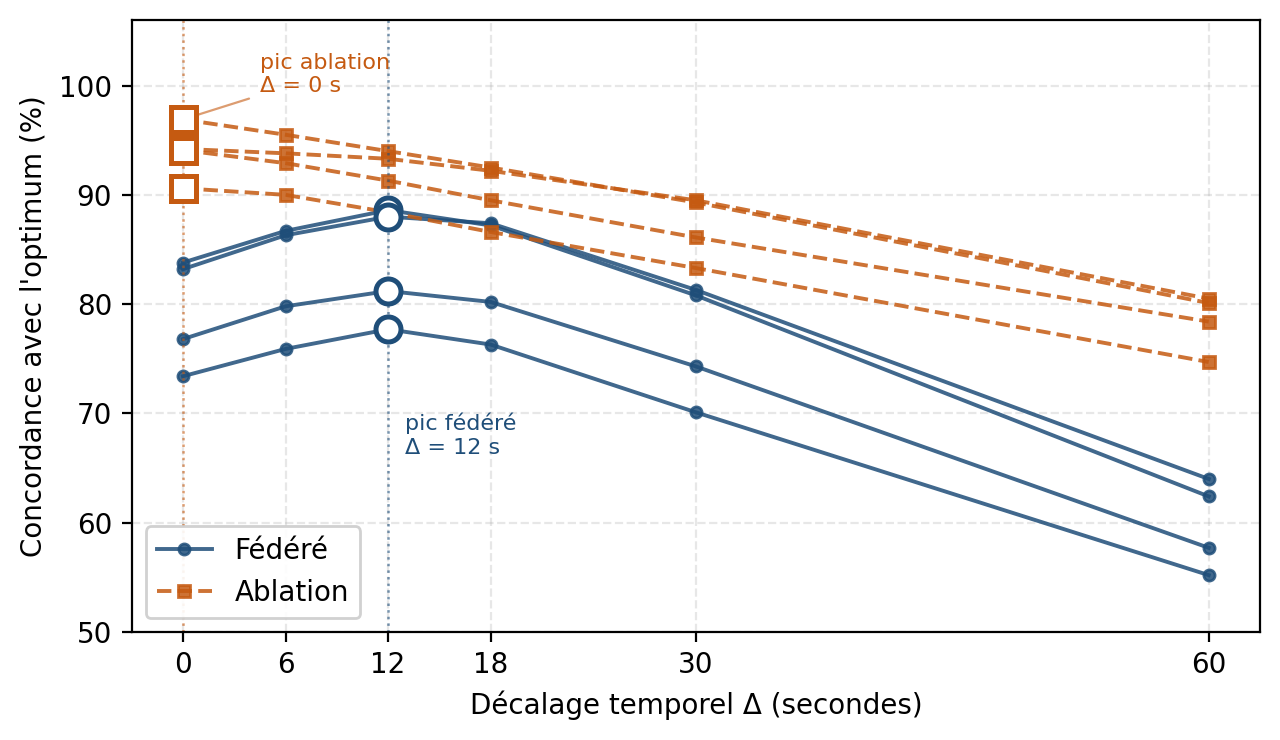
\includegraphics[width=0.95\textwidth]{images/fig_concordance.png}
    \caption{Concordance avec l'optimum selon le décalage temporel $\Delta$. Les cercles évidés marquent le maximum de chaque exécution.}
    \label{fig:concordance}
\end{figure}

Le résultat se reproduit sans exception sur les huit exécutions indépendantes, comme le montre la figure~\ref{fig:concordance}. Les quatre exécutions fédérées atteignent toutes leur maximum de concordance à $\Delta = 12$~s, tandis que les quatre exécutions d'ablation l'atteignent toutes à $\Delta = 0$~s. Aucune exécution ne fait exception et, dans les huit cas, le taux de concordance décroît de manière régulière de part et d'autre du maximum. Cette reproductibilité indique que le phénomène observé ne semble pas dépendre d'une seule exécution ou d'une fenêtre de mesure particulière.

En configuration fédérée, la décision suit donc l'optimum avec un retard d'environ douze secondes, soit deux cycles complets. Le système ne sélectionne pas nécessairement une cible intrinsèquement inadéquate : il tend à sélectionner une cible qui correspond à l'optimum observé deux cycles plus tôt.

Rapporté à la dynamique du banc d'essai, ce retard reste modeste dans l'absolu. Le véhicule progresse à vingt-cinq millimètres par seconde ; en douze secondes, il parcourt donc trois centimètres, alors que le rayon de la zone dans laquelle le seuil de latence est respecté avoisine quinze centimètres. Traverser une telle zone de part en part demande ainsi de l'ordre de deux minutes et le retard de décision en représente environ un dixième. Le système ne se trompe donc pas de région : il présente plutôt un décalage de phase à l'intérieur d'un mouvement qu'il suit correctement par ailleurs.

Cette modestie apparente ne doit toutefois pas conduire à en minimiser l'effet. Douze secondes suffisent pour que le véhicule franchisse une frontière de zone, et c'est précisément aux abords de ces frontières que la décision devient déterminante. Au milieu d'une zone, plusieurs cibles peuvent en effet présenter un comportement comparable. Le retard ne dégrade donc pas nécessairement la qualité de service de manière uniforme : son effet se concentre principalement lors des transitions, lorsque le placement doit s'adapter à l'évolution de la position du véhicule.

L'absence apparente de retard en ablation demande une lecture prudente. Il serait tentant d'en conclure que le mode mono-fournisseur décide plus rapidement. Une autre interprétation, cohérente avec la configuration expérimentale, est que les quatre cibles, toutes situées chez le même fournisseur, offrent moins d'occasions de changement de VM optimale. Un retard de deux cycles peut alors rester difficile à observer, puisque l'optimum n'a, dans de nombreux cas, pas changé pendant cet intervalle. Les résultats ne permettent donc pas d'affirmer que le retard est absent en configuration d'ablation ; ils montrent qu'il n'est pas mis en évidence par cette mesure. Le doublement du nombre de cibles ne crée donc pas nécessairement le retard : il peut également le rendre plus observable.

Ce retard est associé à un coût mesurable. Le classement des violations selon qu'une VM conforme existait ou non au même instant permet de le quantifier :

\begin{table}[H]
    \centering
    \caption{Nature des violations selon la configuration (moyenne sur quatre exécutions par condition)}
    \label{tab:violations-evitables}
    \begin{tabular}{lcc}
        \toprule
        \textbf{Nature des violations} & \textbf{Fédéré} & \textbf{Ablation} \\
        \midrule
        Violations inévitables (aucune VM conforme) & 7,6~\% & 53,2~\% \\
        Violations évitables (une VM conforme existait) & 16,3~\% & 1,7~\% \\
        \bottomrule
    \end{tabular}
\end{table}

En ablation, la majorité des violations est inévitable : aucune des quatre cibles n'était conforme à l'instant considéré et aucun choix parmi les cibles disponibles n'aurait pu éviter la violation. En configuration fédérée, la situation est différente : la proportion de violations inévitables tombe à 7,6~\%, tandis que 16,3~\% du temps correspond à des situations dans lesquelles une cible conforme existait sans avoir été retenue. Ces violations évitables sont compatibles avec l'existence du retard mis en évidence par l'analyse précédente : une cible conforme était disponible, mais elle n'était pas encore sélectionnée au moment considéré.

\textbf{Une cause candidate a été identifiée, puis testée.} L'agrégation des prédictions sur l'horizon repose sur une moyenne pondérée dont les poids décroissent linéairement. Le premier pas prédit reçoit ainsi un poids de 7 sur un total de 28, soit 25~\% de l'ensemble, tandis que le septième n'en reçoit que 3,6~\%. La valeur agrégée est donc davantage influencée par les prédictions les plus proches, ce qui pourrait contribuer à un comportement davantage réactif qu'anticipatif. Un profil de pondération recentré sur les deuxième et troisième pas, correspondant à l'horizon utile de deux cycles, constituait donc une piste de correction cohérente avec le retard observé.

Cette hypothèse n'ayant pas pu être vérifiée pendant la campagne — le principe retenu interdisait de modifier un paramètre entre deux exécutions — elle a fait l'objet d'une exécution supplémentaire menée ultérieurement, sur la même trajectoire et dans la même configuration fédérée. Le profil de pondération y était remplacé par $[3,5,5,4,3,2,1]$, plaçant le maximum sur les deuxième et troisième pas. Le critère de réussite avait été fixé avant l'exécution : le maximum de concordance devait se déplacer vers $\Delta = 6$~s ou $\Delta = 0$~s.

\begin{table}[H]
    \centering
    \caption{Effet du profil de pondération recentré (exécution supplémentaire)}
    \label{tab:run9-horizon}
    \begin{tabular}{lrr}
        \toprule
        \textbf{Indicateur} & \textbf{Campagne (4 exécutions)} & \textbf{Profil recentré} \\
        \midrule
        Maximum de concordance & $\Delta = 12$~s & $\Delta = 12$~s \\
        Concordance à $\Delta = 6$~s & 82,2~\% & 79,3~\% \\
        Concordance à $\Delta = 12$~s & 83,9~\% & 79,8~\% \\
        \addlinespace
        Taux de violation & 23,8~\% (19,9 -- 29,3) & 26,5~\% \\
        Violations évitables & 16,3~\% (12,2 -- 21,8) & 19,2~\% \\
        Migrations / 100 cycles & 7,0 (6,5 -- 7,3) & 6,1 \\
        \bottomrule
    \end{tabular}
\end{table}

\textbf{Le critère n'est pas atteint : le maximum reste à douze secondes.} L'hypothèse selon laquelle la pondération de l'horizon serait la cause du retard n'est donc pas confirmée. Sur les autres indicateurs, l'exécution ne se distingue pas des quatre exécutions fédérées de la campagne : taux de violation et violations évitables restent dans leur étendue respective, et la fréquence des migrations demeure comparable, ce qui écarte au passage un effet oscillatoire du nouveau profil.

Un élément mérite néanmoins d'être relevé sans être surinterprété : l'écart de concordance entre $\Delta = 6$~s et $\Delta = 12$~s, compris entre 1,4 et 1,9 point sur les quatre exécutions de la campagne, tombe à 0,5 point ici. Le maximum s'aplatit sans se déplacer. Cette observation, issue d'une exécution unique et menée avec des modèles de prédiction réentraînés entre-temps, ne permet pas de conclure à un effet partiel de la modification.

\textbf{Le retard de suivi reste donc une limite mesurée dont la cause n'est pas établie.} La formulation retenue ici est délibérément prudente : l'hypothèse la plus immédiate a été testée dans les conditions de la campagne et n'a pas été confirmée, ce qui exclut une explication et en laisse d'autres ouvertes — durée du cycle, délai de propagation des migrations, ou combinaison de plusieurs facteurs. Ce point est repris parmi les pistes d'amélioration en section~\ref{sec:limites-ameliorations}.

\subsection{Stabilité des décisions}
\label{sec:stabilite-decisions}

Une décision juste, mais prise trop fréquemment, peut devenir coûteuse. Chaque migration entraîne le déplacement effectif d'un pod entre deux machines, avec l'interruption de service que cela implique. Un orchestrateur qui basculerait à chaque cycle vers la cible marginalement la mieux classée serait difficilement exploitable, même si chacun de ses choix était localement justifié. La stabilité n'est donc pas une qualité accessoire du système : elle constitue une condition de son utilisabilité.

Trois garde-fous contribuent à cette stabilité. Une marge d'hystérésis exige qu'une cible candidate dépasse la cible active de plus de cinq pour cent en termes de score multicritère avant qu'une migration ne soit envisagée ; en deçà de ce seuil, le système conserve son placement. Un délai de garde interdit toute nouvelle migration pendant les secondes qui suivent la précédente. Enfin, en configuration fédérée, l'arbitre applique une bande morte absolue sur l'écart entre les offres, afin d'éviter un changement de fournisseur lorsqu'un concurrent n'est que marginalement meilleur.

\textbf{Méthode.} Le nombre de migrations effectivement déclenchées a été relevé dans les journaux de décision de chaque exécution. Les durées d'exécution différant sensiblement, les valeurs brutes ne sont pas directement comparables ; elles sont donc rapportées sous forme d'un taux pour cent cycles d'orchestration. En configuration fédérée, le service peut être déplacé par l'un ou l'autre des deux orchestrateurs. Les migrations des deux fournisseurs sont donc cumulées, tandis que le nombre de cycles du premier sert de référence temporelle, les deux orchestrateurs opérant à la même cadence.

\begin{table}[H]
    \centering
    \caption{Fréquence des migrations par condition}
    \label{tab:frequence-migrations}
    \begin{tabular}{llrrr}
        \toprule
        \textbf{Exécution} & \textbf{Condition} & \textbf{Cycles} & \textbf{Migrations} & \textbf{Taux (/100 cycles)} \\
        \midrule
        UC1  & fédéré   & 462 & 30 & 6,5 \\
        FED1 & fédéré   & 475 & 34 & 7,2 \\
        FED2 & fédéré   & 491 & 34 & 6,9 \\
        FED3 & fédéré   & 931 & 68 & 7,3 \\
        \addlinespace
        UC2  & ablation & 406 & 16 & 3,9 \\
        ABL1 & ablation & 402 & 29 & 7,2 \\
        ABL2 & ablation & 566 & 72 & 12,7 \\
        ABL3 & ablation & 630 & 55 & 8,7 \\
        \midrule
        \multicolumn{2}{l}{\textbf{Fédéré} — taux moyen}   & \multicolumn{2}{r}{\textbf{7,0}} & étendue 6,5 -- 7,3 \\
        \multicolumn{2}{l}{\textbf{Ablation} — taux moyen} & \multicolumn{2}{r}{\textbf{8,2}} & étendue 3,9 -- 12,7 \\
        \bottomrule
    \end{tabular}
\end{table}

Aucune configuration ne présente, au regard de ces mesures, de comportement oscillatoire manifeste. Un taux de sept migrations pour cent cycles correspond à environ une migration toutes les quatorze cycles, soit près d'une minute et demie. Cette durée est à rapprocher des deux minutes nécessaires au véhicule pour traverser une zone de conformité. Le rythme des migrations est donc compatible avec la dynamique du déplacement plutôt qu'avec une succession rapide de basculements entre les cibles. Les garde-fous semblent ainsi limiter les migrations excessivement fréquentes dans les deux configurations.

Le premier résultat est contre-intuitif : doubler le nombre de cibles n'augmente pas la fréquence des migrations. On pourrait s'attendre à l'inverse, dans la mesure où un ensemble de choix plus large offre davantage d'occasions de basculer. Le taux moyen est pourtant légèrement inférieur en configuration fédérée qu'en ablation. Une explication possible tient davantage à la qualité et à la disponibilité temporelle des cibles qu'à leur seul nombre : lorsqu'une cible conforme est disponible, elle peut le rester plusieurs cycles, ce qui limite les changements successifs.

Le second résultat concerne la régularité observée entre les exécutions. Les quatre exécutions fédérées s'inscrivent dans un intervalle de 6,5 à 7,3 migrations pour cent cycles, soit une étendue de 0,8 point. Les quatre exécutions d'ablation s'échelonnent de 3,9 à 12,7, soit une étendue de 8,8 points, plus de dix fois supérieure. Alors même que la trajectoire du véhicule est identique d'une exécution à l'autre, le taux de migration varie davantage entre les exécutions en configuration d'ablation que dans la configuration fédérée.

Cette dispersion en ablation n'a pas reçu d'explication établie. L'hypothèse la plus immédiate — selon laquelle un nombre plus faible de cibles conformes conduirait le système à rechercher davantage d'alternatives — ne suffit pas à expliquer les résultats observés. En effet, la proportion de violations inévitables, rapportée en section~\ref{sec:retard-suivi}, est pratiquement identique entre l'exécution présentant le taux de migration le plus faible et celle présentant le taux le plus élevé : 52,9~\% contre 53,0~\%, alors que leurs taux de migration diffèrent d'un facteur supérieur à trois. La cause de cette variabilité reste donc à caractériser et est rapportée comme telle, sans lui attribuer d'explication non vérifiée.

Sous cette réserve, la régularité observée dans la configuration fédérée constitue un résultat favorable : sur les quatre exécutions considérées, la fréquence des migrations varie moins que dans la configuration d'ablation. Ces résultats suggèrent que, dans les conditions évaluées, la décision issue de la négociation entre fournisseurs est moins variable d'une exécution à l'autre que celle prise par un fournisseur isolé.

\newpage
\section{Résultats : fédération}
\label{sec:resultats-federation}

Les sections précédentes ont évalué les composants du système et le comportement d'un fournisseur isolé. Celle-ci répond à la question qui a motivé l'ensemble du travail : la coopération entre fournisseurs indépendants améliore-t-elle effectivement le respect des objectifs de qualité de service ? Trois aspects sont examinés : la réduction du taux de violation (section~\ref{sec:federation-reduit-violation}), la part du gain théoriquement atteignable effectivement capturée (section~\ref{sec:gain-capture}), et le comportement du système lors du passage de relais entre fournisseurs (section~\ref{sec:passage-relais}).

\subsection{La fédération réduit le taux de violation}
\label{sec:federation-reduit-violation}

C'est le résultat central de ce travail. La problématique posée au chapitre~1 supposait qu'un fournisseur seul ne peut pas toujours honorer une intention, et que la coopération avec ses pairs devrait permettre d'y parvenir. Cette hypothèse est ici confrontée à la mesure, sur huit exécutions indépendantes.

\begin{table}[H]
    \centering
    \caption{Taux de violation par exécution}
    \label{tab:taux-violation}
    \begin{tabular}{llrrr}
        \toprule
        \textbf{Exécution} & \textbf{Condition} & \textbf{Durée} & \textbf{Échantillons en violation} & \textbf{Taux} \\
        \midrule
        UC1  & fédéré   & 52,8~min  & 315 / 1\,586  & 19,9~\% \\
        FED1 & fédéré   & 55,7~min  & 422 / 1\,627  & 25,9~\% \\
        FED2 & fédéré   & 57,0~min  & 502 / 1\,712  & 29,3~\% \\
        FED3 & fédéré   & 108,4~min & 656 / 3\,252  & 20,2~\% \\
        \addlinespace
        UC2  & ablation & 40,5~min  & 652 / 1\,215  & 53,7~\% \\
        ABL1 & ablation & 44,3~min  & 701 / 1\,331  & 52,7~\% \\
        ABL2 & ablation & 57,4~min  & 973 / 1\,720  & 56,6~\% \\
        ABL3 & ablation & 63,1~min  & 1\,067 / 1\,894 & 56,3~\% \\
        \midrule
        \multicolumn{2}{l}{\textbf{Fédéré} — moyenne}   & \multicolumn{2}{r}{\textbf{23,8~\%}} & $\sigma$ = 4,6~pt \\
        \multicolumn{2}{l}{\textbf{Ablation} — moyenne} & \multicolumn{2}{r}{\textbf{54,8~\%}} & $\sigma$ = 1,9~pt \\
        \bottomrule
    \end{tabular}
\end{table}

L'écart est de \textbf{31,0 points} en faveur de la configuration fédérée, soit une réduction de 57~\% du temps passé en violation.

\begin{figure}[H]
    \centering
    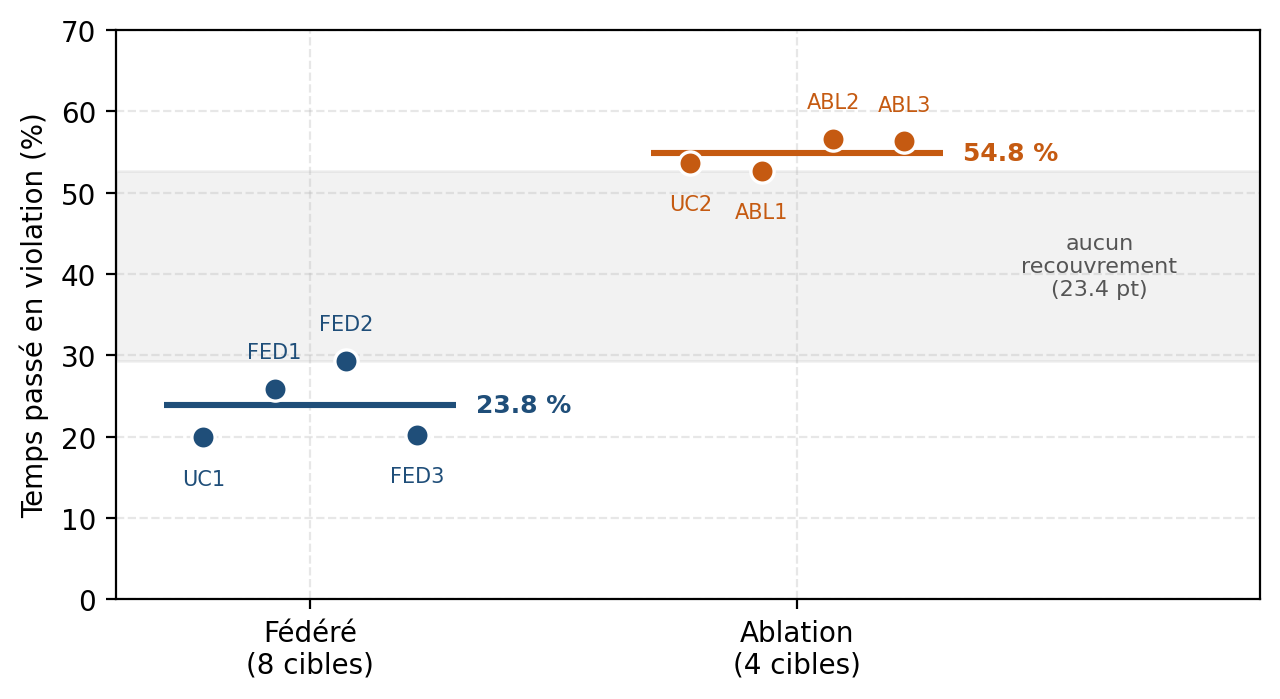
\includegraphics[width=0.92\textwidth]{images/fig_violation.png}
    \caption{Taux de violation des huit exécutions. Les traits horizontaux indiquent la moyenne de chaque condition ; la bande grisée matérialise l'intervalle où aucune exécution ne tombe.}
    \label{fig:violation}
\end{figure}

\textbf{Les deux groupes ne se recouvrent pas.} La pire exécution fédérée (29,3~\%) reste inférieure de plus de vingt-trois points à la meilleure exécution d'ablation (52,7~\%). Cette séparation stricte est une propriété forte : elle signifie que le classement des huit exécutions place les quatre exécutions fédérées avant les quatre exécutions d'ablation, sans exception.

Le test exact de Mann-Whitney, justifié en section~\ref{sec:protocole-metriques}, confirme cette lecture : $U = 16{,}0$ et $p = 0{,}0286$. La statistique $U$ atteint sa valeur maximale, ce qui correspond précisément à l'absence de recouvrement entre les deux groupes. La valeur de $p$ obtenue est la plus petite atteignable avec quatre observations par condition : le résultat est significatif au seuil de 5~\%, et il l'est autant que la taille de l'échantillon le permet. Aucune configuration de ces huit mesures ne pourrait produire une p-valeur inférieure.

\textbf{Ce que ce résultat établit, et ce qu'il n'établit pas.} Il établit que, sur ce banc d'essai et pour cette trajectoire, l'accès aux cibles d'un second fournisseur réduit très significativement le temps passé en violation. La seule différence entre les deux conditions étant l'activation de la fédération — même trajectoire, même seuil, même code — l'écart lui est attribuable.

Il n'établit pas que le gain provient de la qualité de la décision. La section~\ref{sec:gain-capture} montre au contraire qu'il provient d'abord de l'élargissement de la couverture physique : avec quatre cibles seulement, aucune n'est conforme plus de la moitié du temps, et aucun algorithme, si bon soit-il, ne pourrait éviter ces violations.

\textbf{Trois réserves accompagnent ce résultat.}

D'abord, quatre exécutions par condition suffisent à établir une différence, non à la caractériser. Elles bornent une moyenne et une dispersion, mais ne disent rien de la forme de la distribution sous-jacente et n'autorisent aucun diagnostic de valeur aberrante. Les exécutions fédérées diffèrent entre elles de 9,4 points, et cette dispersion n'a pas reçu d'explication établie.

Ensuite, les deux chemins de décision ne partagent pas exactement la même politique de dernier recours. Lorsque aucune cible ne satisfait le contrat, le chemin fédéré déclare l'intention infaisable plutôt que de retenir une offre non conforme — un fournisseur n'exporte jamais vers un pair un placement qu'il sait en infraction — tandis que le chemin mono-fournisseur retient la moins mauvaise cible disponible. Cette asymétrie est délibérée, mais elle signifie que les deux conditions ne diffèrent pas uniquement par le nombre de cibles. Son effet reste toutefois borné : elle ne s'applique que lorsque aucune cible conforme n'existe, et l'écart mesuré est d'un ordre de grandeur supérieur à toute contribution plausible de ce mécanisme.

Enfin, une neuvième exécution fédérée a été menée après la campagne, avec un profil de pondération modifié (section~\ref{sec:retard-suivi}). Exécutée avec un code différent des huit autres, elle n'entre ni dans les moyennes rapportées ici ni dans le test statistique.

\subsection{Part du gain atteignable capturée}
\label{sec:gain-capture}

Le résultat précédent établit un écart entre les deux conditions ; il ne dit rien de la part de cet écart imputable à la qualité des décisions plutôt qu'à l'étendue du choix disponible. Deux bornes permettent de situer chaque système entre ce qu'aucun algorithme ne pourrait éviter et ce qu'un placement figé, sans aucune décision, obtiendrait déjà.

\textbf{Méthode.} Pour chaque instant, la borne oracle retient la VM offrant la plus faible latence à cet instant précis, ce qu'aucun système réel ne peut faire puisqu'elle suppose une connaissance parfaite et instantanée de l'état de toutes les cibles. La borne du meilleur placement statique retient, sur toute l'exécution, la VM unique qui minimise le taux de violation si le service y restait sans jamais migrer — c'est le comportement d'un ordonnanceur Kubernetes ordinaire, qui place une fois et ne réévalue pas.

\begin{table}[H]
    \centering
    \caption{Bornes de comparaison — configuration fédérée}
    \label{tab:bornes-federe}
    \begin{tabular}{lrrrr}
        \toprule
        \textbf{Exécution} & \textbf{Oracle} & \textbf{Système} & \textbf{Meilleur statique} & \textbf{Gain capturé} \\
        \midrule
        UC1  &  7,6~\% & 19,9~\% & 81,8~\% & 83~\% \\
        FED1 &  7,4~\% & 25,9~\% & 80,7~\% & 75~\% \\
        FED2 &  7,5~\% & 29,3~\% & 82,2~\% & 71~\% \\
        FED3 &  7,6~\% & 20,2~\% & 82,7~\% & 83~\% \\
        \midrule
        \textbf{Moyenne} & \textbf{7,5~\%} & \textbf{23,8~\%} & \textbf{81,9~\%} & \textbf{78~\%} \\
        \bottomrule
    \end{tabular}
\end{table}

\begin{table}[H]
    \centering
    \caption{Bornes de comparaison — configuration d'ablation}
    \label{tab:bornes-ablation}
    \begin{tabular}{lrrrr}
        \toprule
        \textbf{Exécution} & \textbf{Oracle} & \textbf{Système} & \textbf{Meilleur statique} & \textbf{Gain capturé} \\
        \midrule
        UC2  & 52,9~\% & 53,7~\% & 82,3~\% & 97~\% \\
        ABL1 & 51,8~\% & 52,7~\% & 83,0~\% & 97~\% \\
        ABL2 & 53,0~\% & 56,6~\% & 83,4~\% & 88~\% \\
        ABL3 & 54,9~\% & 56,3~\% & 84,2~\% & 95~\% \\
        \midrule
        \textbf{Moyenne} & \textbf{53,1~\%} & \textbf{54,8~\%} & \textbf{83,2~\%} & \textbf{94~\%} \\
        \bottomrule
    \end{tabular}
\end{table}

\begin{figure}[H]
    \centering
    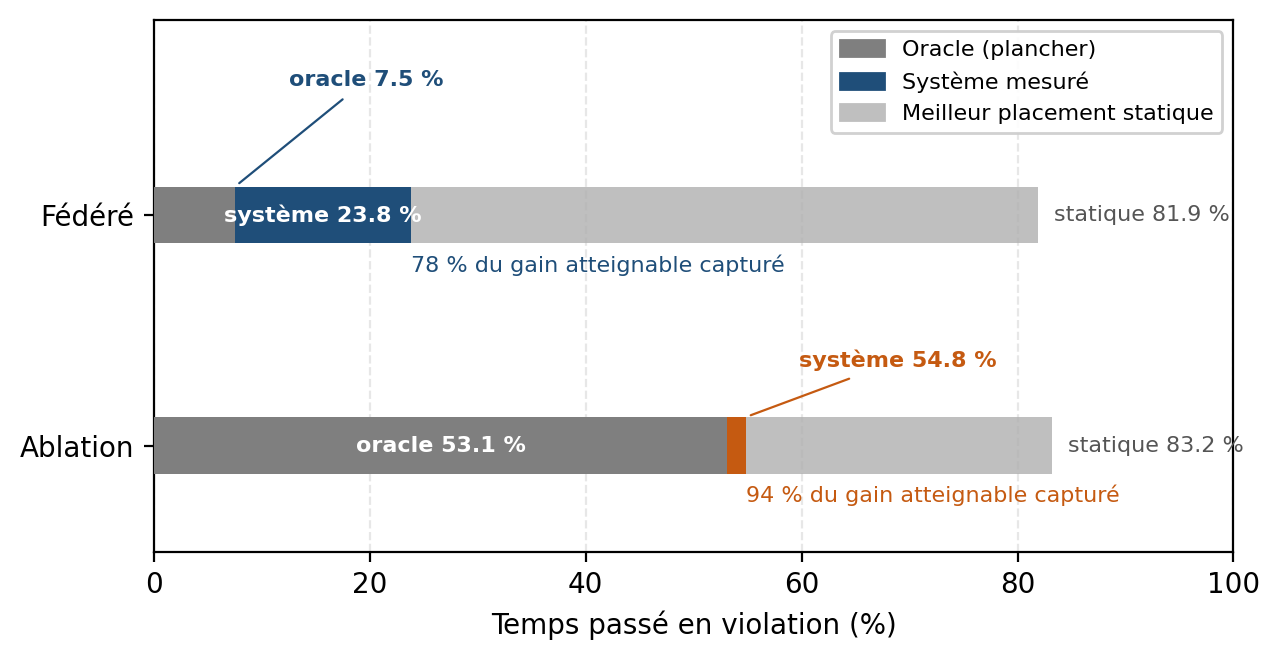
\includegraphics[width=0.95\textwidth]{images/fig_bornes.png}
    \caption{Position du système entre ses deux bornes, par condition. La fédération abaisse l'oracle de 53,1~\% à 7,5~\% : c'est l'atteignable lui-même qui se déplace.}
    \label{fig:bornes}
\end{figure}

\textbf{L'ablation capture presque tout son gain atteignable ; le fédéré, non.} En configuration d'ablation, le système mesuré s'écarte de son propre oracle de 0,8 à 3,6 points seulement selon l'exécution — il capture en moyenne 94~\% du gain théoriquement atteignable compte tenu des quatre cibles disponibles. En configuration fédérée, cet écart monte à 12,3--21,8 points, pour une capture moyenne de 78~\%.

Cette asymétrie répond directement à la question laissée ouverte en section~\ref{sec:federation-reduit-violation} : le gain observé ne provient pas d'une décision meilleure en fédéré qu'en ablation — c'est l'inverse qui est mesuré. Il provient de l'élargissement du choix disponible : doubler le nombre de cibles déplace l'oracle de 53,1~\% à 7,5~\%, soit 45,6 points gagnés par la seule extension de la couverture, avant même toute décision.

\textbf{Ce que cet écart de capture révèle.} Que le fédéré capture une part moindre de son gain atteignable n'indique pas un défaut de conception spécifique à la fédération : il est cohérent avec le retard de suivi de douze secondes mesuré en section~\ref{sec:retard-suivi}, qui n'affecte que la configuration fédérée. FED1 et FED2, les deux exécutions où cet écart est le plus marqué (75~\% et 71~\%), sont aussi celles où la proportion de violations évitables est la plus élevée (section~\ref{sec:retard-suivi}) — cohérence supplémentaire entre deux mesures obtenues par des méthodes indépendantes.

\subsection{Comportement lors du passage de relais}
\label{sec:passage-relais}

Le mécanisme de fédération n'est pertinent que si le passage du service d'un fournisseur à l'autre se déroule sans ambiguïté ni retard excessif. Cette section illustre ce mécanisme sur un exemple réel, tiré des journaux de l'exécution FED3.

\textbf{Le déclencheur.} Au cycle 3, l'arbitre de provider-2 propose \texttt{edge2} avec un Gap Grade de $-0{,}7151$, contre $-0{,}0239$ pour le tenant en place chez provider-1 — un écart qui dépasse la bande morte de $0{,}05$ retenue pour éviter les changements de fournisseur marginaux. La migration est déclenchée.

\begin{table}[H]
    \centering
    \caption{Séquence d'un passage de relais réel (FED3, cycle 3)}
    \label{tab:passage-relais}
    \begin{tabular}{lp{7.5cm}}
        \toprule
        \textbf{Horodatage} & \textbf{Événement} \\
        \midrule
        12:20:52 & Décision \texttt{migrate edge1 → edge2} enregistrée côté provider-1 \\
        12:20:53 & Migration \texttt{kubectl} exécutée (190~ms) ; \texttt{/award} envoyé à provider-2 \\
        12:20:54 & \texttt{/award} livré ; provider-1 passe en \textbf{STANDBY} ; provider-2 passe en \textbf{ACTIF} \\
        12:20:56 & Une synchronisation \texttt{kubectl} périmée arrive côté provider-2 ; ignorée grâce à la fenêtre de grâce, le rôle ACTIF est conservé \\
        \bottomrule
    \end{tabular}
\end{table}

\textbf{Le rôle de la fenêtre de grâce.} Deux secondes après avoir reçu l'attribution, provider-2 reçoit une resynchronisation \texttt{kubectl} qui reflète encore l'état antérieur à la migration. Sans protection, cette resynchronisation aurait pu ramener provider-2 en STANDBY alors qu'il vient tout juste de prendre le service — un split-brain de courte durée, où aucun des deux fournisseurs ne se considérerait actif. La fenêtre de grâce qui suit chaque \texttt{award} neutralise précisément ce cas : le journal l'indique explicitement (\og~synchronisation kubectl périmée ignorée, fenêtre de grâce award, rôle conservé : ACTIF~\fg{}).

\textbf{Durée totale.} Depuis la décision jusqu'à la confirmation du nouveau rôle, la séquence complète prend environ 4,3 secondes sur cet exemple, migration \texttt{kubectl} et transmission de l'attribution comprises — un ordre de grandeur inférieur au cycle d'orchestration de six secondes, ce qui évite qu'un passage de relais empiète sur le suivant.

\newpage
\section{Synthèse et limites}
\label{sec:synthese-limites}

\subsection{Bilan par rapport à la problématique}
\label{sec:bilan-problematique}

La problématique posée au chapitre~1 interrogeait la capacité d'un fournisseur isolé à honorer une intention de qualité de service, et proposait la coopération entre fournisseurs comme réponse. Les résultats de ce chapitre y répondent, avec les nuances que la mesure impose.

\textbf{La chaîne fonctionne de bout en bout.} Une intention en langage naturel est traduite en contrat SLO pondéré (section~\ref{sec:fidelite-interpretation}), y compris sur des formulations non conçues pour le système ; les deux demandes hors périmètre sont déclinées plutôt que mal interprétées (section~\ref{sec:comportement-repli}). Le contrat pilote ensuite une décision locale informée par la prédiction (section~\ref{sec:qualite-prediction}) et, potentiellement, par une métrique secondaire découverte (section~\ref{sec:validation-mi}).

\textbf{La fédération répond positivement à la problématique.} L'accès aux cibles d'un second fournisseur réduit le taux de violation de 54,8~\% à 23,8~\% (section~\ref{sec:federation-reduit-violation}), un écart significatif au seuil de 5~\%. Ce gain provient majoritairement de l'élargissement du choix disponible plutôt que d'une décision plus fine : le système capture 94~\% de son gain atteignable en ablation contre 78~\% en fédéré (section~\ref{sec:gain-capture}) — la fédération élargit ce qui est atteignable, plus qu'elle n'améliore la façon de l'atteindre.

\textbf{Cette réponse reste bornée.} Un retard de suivi de douze secondes (section~\ref{sec:retard-suivi}) et une dispersion inter-exécutions non expliquée (section~\ref{sec:limites-ameliorations}) limitent la part du gain effectivement capturée. La coopération entre fournisseurs n'élimine donc pas toute violation ; elle déplace substantiellement la limite de ce qui est atteignable, et le système en capture une majorité, sans encore l'épuiser.

\subsection{Limites et pistes d'amélioration}
\label{sec:limites-ameliorations}

Cette section rassemble les limites identifiées au fil du chapitre, avec pour chacune ce qui a déjà été testé, ce qui reste ouvert, et pourquoi certaines ne sont pas traitées comme des défauts à corriger.

\textbf{Le retard de suivi.} L'hypothèse des poids d'horizon (section~\ref{sec:retard-suivi}) a été testée et n'a pas été confirmée. Deux pistes recensées avant la campagne restent, elles, non testées : réduire la période du cycle (6~s~$\rightarrow$~3~s), qui diviserait mécaniquement le retard mais recouple l'ensemble des grandeurs temporelles du banc (horizon de prédiction, fenêtre d'historique, cooldown) et exige une étude de dimensionnement préalable — cette modification est reportée à une itération ultérieure, une fois cette étude menée ; et réduire le délai de garde entre deux migrations, plus simple mais avec un risque d'oscillation à surveiller. Une piste supplémentaire a été identifiée après la campagne : le temps de négociation entre fournisseurs, mesuré entre 2,6 et 3,2 secondes lorsqu'elle a lieu, pousse certains cycles au-delà du budget nominal de 6~s — cohérent avec le retard mesuré, sans être confirmé comme cause unique. L'examen du code a révélé qu'une connexion réseau neuve était ouverte à chaque négociation, sans réutilisation. Le correctif correspondant, mesuré sur trente négociations consécutives dans les conditions du banc, ramène le temps de négociation de 2\,392~ms à 881~ms en médiane, soit une réduction de 63~\%. Cette accélération est établie ; son effet sur le retard de suivi ne l'est pas, faute d'un nombre d'exécutions suffisant pour le distinguer de la variabilité déjà observée entre exécutions.

\textbf{Le plancher du Gap Grade.} La borne \texttt{DELTA\_FLOOR} limite l'écart normalisé à $-1$ au minimum. Sans elle, un excédent extrême sur un critère secondaire peut dominer la somme pondérée et l'emporter sur un critère primaire pourtant plus fragile — l'exemple illustratif suivant, construit pour deux SLO pondérés (latence $< 65$~ms, poids $0{,}6$ ; CPU disponible $\geq 2{,}5$~cœurs, poids $0{,}4$), le montre.

\begin{table}[H]
    \centering
    \caption{Exemple illustratif — deux VM conformes}
    \label{tab:floor-exemple-entree}
    \begin{tabular}{lccc}
        \toprule
        \textbf{VM} & \textbf{Latence} & \textbf{CPU disponible} & \textbf{Conforme} \\
        \midrule
        cloud1 & 60~ms & 12,8~cœurs & oui \\
        edge2  & 32~ms &  3,2~cœurs & oui \\
        \bottomrule
    \end{tabular}
\end{table}

\begin{table}[H]
    \centering
    \caption{Écarts normalisés, avant et après plancher}
    \label{tab:floor-exemple-ecarts}
    \begin{tabular}{lrrr}
        \toprule
        \textbf{VM} & $\delta_{\text{latence}}$ & $\delta_{\text{CPU}}$ (brut) & $\delta_{\text{CPU}}$ (planché) \\
        \midrule
        cloud1 & $-0{,}077$ & $-4{,}120$ & $-1{,}000$ \\
        edge2  & $-0{,}508$ & $-0{,}280$ & $-0{,}280$ \\
        \bottomrule
    \end{tabular}
\end{table}

\begin{table}[H]
    \centering
    \caption{Gap Grade résultant, avant et après plancher}
    \label{tab:floor-exemple-resultat}
    \begin{tabular}{lrr}
        \toprule
        \textbf{VM} & \textbf{Sans plancher} & \textbf{Avec plancher} \\
        \midrule
        cloud1 & $-0{,}196$ \textbf{(gagne)} & $-0{,}083$ \\
        edge2  & $-0{,}140$ & $-0{,}140$ \textbf{(gagne)} \\
        \bottomrule
    \end{tabular}
\end{table}

Sans plancher, cloud1 l'emporte : son excédent de CPU écrase la somme pondérée malgré une marge de latence de seulement 5~ms sur un seuil de 65~ms. Avec plancher, edge2 l'emporte — la VM dont la marge est la plus confortable sur le critère le plus pondéré. Le plancher reste une limite au sens strict — il efface une information réelle sur un critère pris isolément — mais il constitue une correction nécessaire au comportement global de l'arbitrage, pas un défaut à corriger.

\textbf{Dispersion inter-exécutions.} Les quatre exécutions fédérées diffèrent entre elles de 9,4 points de taux de violation (section~\ref{sec:federation-reduit-violation}), sans explication établie.

\textbf{Vérification FED1/ABL2.} Deux exécutions de la campagne (FED1, ABL2) avaient fait l'objet d'un doute sur un réentraînement involontaire du modèle ML en cours de run. Vérification faite sur l'erreur de prédiction de latence, tranche par tranche : aucune cassure détectée après la période d'échauffement initiale déjà documentée — l'erreur reste stable et basse jusqu'à la fin des deux exécutions. Cette vérification ne couvre que la prédiction de latence ; elle ne permet pas d'exclure un effet sur les décisions elles-mêmes.

\textbf{Fédération sur deux machines physiques distinctes.} Cette configuration reste bloquée par une limitation de \texttt{launch\_provider.py}, non résolue au moment de la rédaction.

\newpage
\section{Conclusion}
\label{sec:tests-conclusion}

Ce chapitre a soumis xQoS à l'épreuve de la mesure, sur l'infrastructure réelle du LAAS-CNRS plutôt qu'en simulation. Deux échelles distinctes ont structuré cette évaluation : la décision locale, prise par un seul fournisseur à partir de ses propres cibles, et la décision fédérée, qui ouvre ce choix à un pair par négociation.

À l'échelle locale, la traduction d'intention, la prédiction et la découverte de métriques secondaires fonctionnent de bout en bout, avec des limites précisément mesurées plutôt que supposées : une découverte MI d'abord invalidée par le banc d'essai puis validée après correction (section~\ref{sec:validation-mi}), un retard de suivi de deux cycles dont une cause candidate a été testée et écartée (section~\ref{sec:retard-suivi}), un plancher de score dont l'effet a été démontré nécessaire plutôt que simplement toléré (section~\ref{sec:limites-ameliorations}).

À l'échelle fédérée, le résultat central tient en une phrase : ouvrir la décision à un second fournisseur réduit le temps passé en violation de plus de moitié, un écart significatif malgré la petite taille de l'échantillon. Ce gain s'explique d'abord par la couverture physique élargie, et seulement ensuite par la qualité de la décision (section~\ref{sec:gain-capture}) — une distinction que seule la mesure, et non l'intuition, pouvait établir.

Ces résultats répondent à la problématique du chapitre~1 sans la clore (section~\ref{sec:bilan-problematique}) : ils établissent qu'une fédération d'intent-based orchestrators réduit mesurablement les violations de qualité de service sur ce banc d'essai, et documentent avec la même rigueur ce qui reste à améliorer.


\renewcommand\bibname{Webography}
\clearpage
\addcontentsline{toc}{chapter}{Webographie}
\bibliographystyle{ieeetr}
\bibliography{references}

\end{document}
